%%%%%%%%%%%%%%%%%%%%%%%%%%%%%%%%%%%%%%%%%%  不使用 authblk 包制作标题  %%%%%%%%%%%%%%%%%%%%%%%%%%%%%%%%%%%%%%%%%%%%%%
%-------------------------------PPT Title-------------------------------------
\title{线性响应理论}
%-----------------------------------------------------------------------------
%----------------------------Author & Date------------------------------------

%\author[\textrm{Jun\_Jiang}]{姜\;\;骏\inst{}} %[]{} (optional, use only with lots of authors)
%% - Give the names in the same order as the appear in the paper.
%% - Use the \inst{?} command only if the authors have different
%%   affiliation.
\institute[BCC]{\inst{}%
%\institute[Gain~Strong]{\inst{}%
\vskip -20pt 北京市计算中心}
%\vskip -20pt {\large 格致斯创~科技}}
\date[\today] % (optional, should be abbreviation of conference name)
{%	{\fontsize{6.2pt}{4.2pt}\selectfont{\textcolor{blue}{E-mail:~}\url{jiangjun@bcc.ac.cn}}}
\vskip 45 pt {\fontsize{8.2pt}{6.2pt}\selectfont{%清华大学\;\;物理系% 报告地点
	\vskip 5 pt \textrm{2023.08.22}}}
}

%% - Either use conference name or its abbreviation
%% - Not really information to the audience, more for people (including
%%   yourself) who are reading the slides onlin%%   yourself) who are reading the slides onlin%%   yourself) who are reading the slides onlineee
%%%%%%%%%%%%%%%%%%%%%%%%%%%%%%%%%%%%%%%%%%%%%%%%%%%%%%%%%%%%%%%%%%%%%%%%%%%%%%%%%%%%%%%%%%%%%%%%%%%%%%%%%%%%%%%%%%%%%

\subject{}
% This is only inserted into the PDF information catalog. Can be left
% out.
%\maketitle
\frame
{
%	\frametitle{\fontsize{9.5pt}{5.2pt}\selectfont{\textcolor{orange}{“高通量并发式材料计算算法与软件”年度检查}}}
\titlepage
}
%-----------------------------------------------------------------------------

%------------------------------------------------------------------------------列出全文 outline ---------------------------------------------------------------------------------
%\section*{}
%\frame[allowframebreaks]
%{
%  \frametitle{Outline}
%%  \frametitle{\textcolor{mycolor}{\secname}}
%  \tableofcontents%[current,currentsection,currentsubsection]
%}
%%在每个section之前列出全部Outline
%%类似的在每个subsection之前列出全部Outline是\AtBeginSubsection[]
%\AtBeginSection[]
%{
%  \frame<handout:0>%[allowframebreaks]
%  {
%    \frametitle{Outline}
%%全部Outline中,本部分加亮
%    \tableofcontents[current,currentsection]
%  }
%}

%-----------------------------------------------PPT main Body------------------------------------------------------------------------------------
\small
%\section{\rm{VASP~}软件中\rm{PAW~}计算的实现}
%\frame
%
%	\frametitle{\textrm{VASP}计算的特色}
%	相比于与普通的第一原理计算软件,\textrm{VASP}很好地平衡了计算效率和精度的问题,总的来说,\textrm{VASP}主要通过这几个特色保证了计算的高效能
%	\begin{itemize}
%	     \item 迭代与优化算法的多样性\\
%		     本质上电荷密度迭代 \textrm{\&\&} 体系总能量优化是相同的优化问题,采用了类似的算法\upcite{CMS6-15_1996,PRB54-11169_1996}:\\
%			\textcolor{blue}{\textrm{Pseudo-Newton、Conjugate-Gradient、Broyden~mix、damping-factor、RMM-DIIS}}
%	     \item 尽可能采用局域基(原子轨道基)函数:~\\
%		     \textcolor{blue}{\textrm{LREAL}}=\textcolor{red}{\textrm{.TRUE.}}\\
%			优化的投影函数也尽可能在实空间表示
%	     \item \textrm{PAW}原子数据集:\textcolor{blue}{优异的赝势}\upcite{PRB59-1758_1999}
%	\end{itemize}
%}
\section{固体光学性质与能带跃迁}
%\subsection{固体光学常数的基本关系}
\frame
{
	\frametitle{固体光学常数间的基本关系}
	光(电磁波)通过固体材料时,电磁波将与固体中的电子、原子(离子)间相互作用,因此发生光吸收
\begin{figure}[h!]
	\vspace{-3pt}
\centering
\animategraphics[autoplay, loop, height=2.25in, width=3.6in,viewport= 15 30 570 515,clip]{1}{Figures/Light-wave-}{0}{30}
%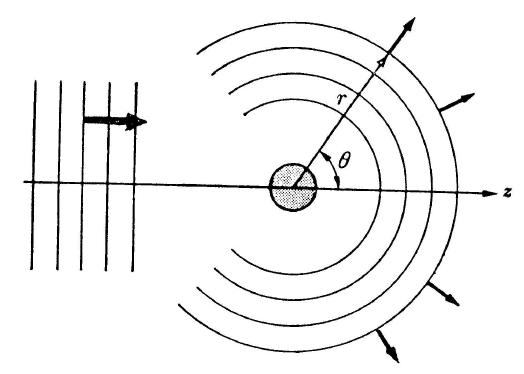
\includegraphics[height=1.29in,width=1.91in,viewport=0 0 400 275,clip]{Figures/Pseudo-scatter.jpg}
\caption{\fontsize{5.5pt}{4.2pt}\selectfont{\textrm{Schematic illustration of electromagnetic wave propagation.}}}%(与文献\cite{EPJB33-47_2003}图1对比)
\label{Light-Wave}
\end{figure}
}

\frame{
	\frametitle{固体光学常数间的基本关系}
	\begin{itemize}
		\item 角频率为$\omega$的电磁波(横波)在均匀介质中传播(设为$x$方向)
			\begin{displaymath}
				\mathbf{E}(\vec r,t)=E(z)\mathrm{e}^{-\mathrm{i}\omega t}(0,0,1)\qquad\mathbf{E}\perp x
			\end{displaymath}
			根据\textrm{Maxwell~}方程,可有电场与电流密度的基本关系
			\begin{displaymath}
				\frac{\mathrm{d}^2E(z)}{\mathrm{d}z^2}=-\frac{\omega^2}{c^2}E(z)-\frac{4\pi\mathrm{i}\omega}{c^2}J(z)
			\end{displaymath}
		\item 引入复数电导率$\sigma(\sigma)=\sigma_1(\omega)+\mathrm{i}\sigma_2(\omega)$
			\begin{displaymath}
				J(z)=\sigma(\omega)E(z)=\sigma_1(\omega)E(z)+\mathrm{i}\sigma_2(\omega)E(z)
			\end{displaymath}
			吸收介质中电流$\mathbf{j}$分为两部分,一部分与$\mathbf{E}$相位差$90^{\circ}$,称为\textcolor{magenta}{极化电流},一部分与电场$\mathbf{E}$同相位,称为\textcolor{magenta}{传导电流}\\
			\textcolor{red}{注意}:~极化电流与电场相位差$90^{\circ}$,在一个周期平均电场做工为零,不消耗电磁场能量
	\end{itemize}
}

\frame
{
	\frametitle{固体光学常数间的基本关系}
	\begin{itemize}
		\item 当载流子迁移距离比电磁波的波长小得多时(长波极限),可忽略电磁波在空间变化的影响
			\begin{displaymath}
				\frac{\mathrm{d}^2E(z)}{\mathrm{d}z^2}=-\frac{\omega^2}{c^2}\left[ 1+\frac{4\pi\mathrm{i}\omega\sigma(\omega)}{\omega} \right]E(z)
			\end{displaymath}
		可解得电磁波在介质内的衰减
		\begin{displaymath}
			E(z)=E_0\mathrm{e}^{\mathrm{i}(\omega/c)Nz}
		\end{displaymath}
		这里$N$是复数折射率,满足
		\begin{displaymath}
			N^2=1+\frac{4\pi\mathrm{i}\sigma(\omega)}{\omega} 
		\end{displaymath}
		\item 复数折射写成$N=n+\mathrm{i}k$,其中$n$是折射指数,$k$是消光系数,因此
			\begin{displaymath}
				E(z)=E_0\mathrm{e}^{\mathrm{i}(\omega/c)nz}\mathrm{e}^{-(\omega/c)kz}
			\end{displaymath}
			因此电磁波在介质中传播速度$c/n$,透射深度$\delta(\omega)=\frac{c}{\omega k(\omega)}$
	\end{itemize}
}

\frame
{
	\frametitle{固体光学常数间的基本关系}
	\begin{itemize}
		\item 吸收系数
			\begin{displaymath}
				\alpha(\omega)=\frac{2\omega k(\omega)}c\equiv\frac2{\delta(\omega)}
			\end{displaymath}
		\item 电磁波在介质中传播,根据介电函数和复数折射率的关系$N^2=\varepsilon$,因此
			\begin{displaymath}
				\varepsilon_1=n^2-k^2\qquad\varepsilon_2=2nk
			\end{displaymath}
			相应地
			\begin{displaymath}
				n^2=\frac12(\varepsilon_1+\sqrt{\varepsilon_1^2+\varepsilon_2^2})\quad k^2=\frac12(-\varepsilon_1+\sqrt{\varepsilon_1^2+\varepsilon_2^2})
			\end{displaymath}
			根据等式$\varepsilon(\omega)=1+\dfrac{4\pi\mathrm{i}\sigma(\omega)}{\omega}$有
			\begin{displaymath}
				\varepsilon_1=1-\frac{4\pi\sigma_2(\omega)}{\omega}\qquad\varepsilon_2=\frac{4\pi\sigma_1(\omega)}{\omega} 
			\end{displaymath}
			\textcolor{red}{注意}:~\textcolor{blue}{确定介电函数虚部与电导率实部间的关系}
	\end{itemize}
}

\frame
{
	\frametitle{固体光学常数间的基本关系}
	\begin{itemize}
		\item 电磁波垂直入射时,反射波与入射波分别为
\begin{figure}[h!]
\centering
%\hspace*{-10pt}
\vspace*{-0.4in}
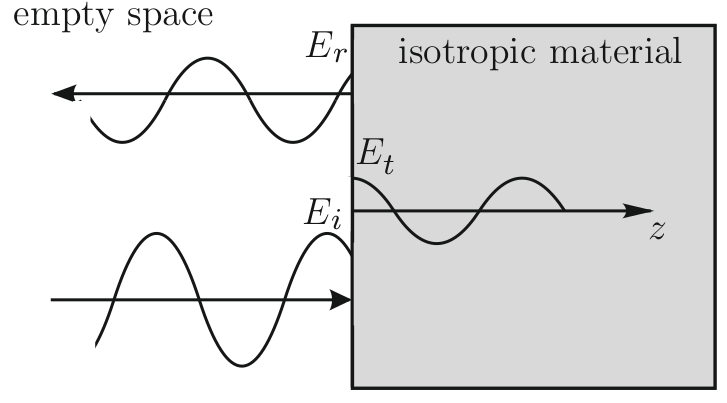
\includegraphics[height=1.2in,width=1.8in,viewport=0 0 750 600,clip]{Figures/Optic-reflect.png}
\caption{\fontsize{5.5pt}{4.2pt}\selectfont{\textrm{Schematic representation of incident, reflected and transmitted electromagnetic\\ wave at the surface.}}}%
\label{Optic-reflect}
\end{figure} 
			\begin{displaymath}
				\begin{aligned}
					&E(z)=E_t\mathrm{e}^{\mathrm{i}(\omega/c)Nz}\quad z>0\\
					&E(z)=E_i\mathrm{e}^{\mathrm{i}(\omega/c)z}+E_r\mathrm{e}^{-\mathrm{i}(\omega/c)z}\quad z<0\\
				\end{aligned}
			\end{displaymath}
			反射率$R$可以表示为
			\begin{displaymath}
				R=\left|\frac{E_r}{E_i}\right|^2=\left|\frac{1-N}{1+N}\right|^2=\frac{(n-1)^2+k^2}{(n+1)^2+k^2}
			\end{displaymath}
	\end{itemize}
}

\subsection{载流子与\rm{Lorentz-Drude}模型}
%\subsection{光子与电子的激发}
\frame
{
	\frametitle{光子与电子的激发}
	电磁波在介质中的传播,伴随了光子与介质中电子的相互作用
\begin{figure}[h!]
\centering
\vspace*{-10pt}
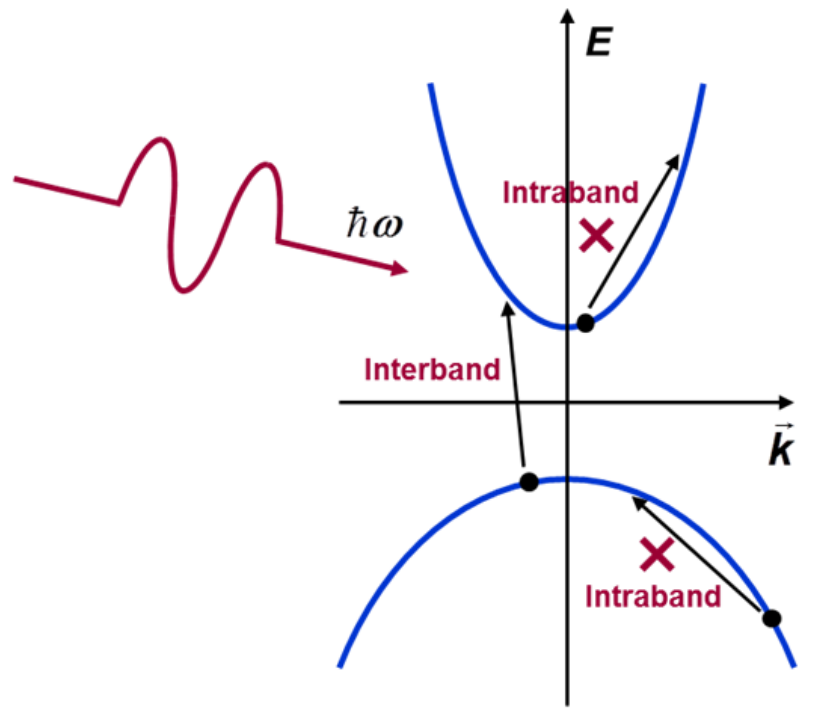
\includegraphics[height=2.3in,width=2.2in,viewport=0 0 800 800,clip]{Figures/Inter-Intra_band-transition.png}
\caption{\fontsize{5.5pt}{4.2pt}\selectfont{\textrm{Schematic representation of interaction of photons and the electrons in the semiconductor.}}}%
\label{Optic-transition}
\end{figure} 
}

\frame
{
	\frametitle{光子与电子的激发}
	粒子间相互作用遵守能量守恒与动量守恒:~\\
	假设介质中的电子初始态为$\vec k_i$,对应的能量为$E_n(\vec k_i)$,电子吸收入射光子跃迁到终态$\vec k_f$,能量变为$E_m(\vec k_f)$,则有
	\begin{itemize}
		\item \textcolor{blue}{能量守恒}
			\begin{displaymath}
				E_m(\vec k_f)=E_n(\vec k_i)+\hbar\omega
			\end{displaymath}
			$\hbar\omega$是入射光子能量
		\item \textcolor{blue}{动量守恒}
			\begin{displaymath}
				\vec k_f=\vec k_i+\vec q
			\end{displaymath}
			$\vec q$是入射光子的动量
	\end{itemize}
	具体计算过程中,考虑光子引起的介质中电子的状态变化,采取了一系列的简化
}

\frame
{
	\frametitle{电场中的自由电子:~\textrm{Lorentz}模型}
	\begin{itemize}
		\item 载流子在外电场$\mathbf{E}(\vec r,t)=\mathbf{E}_0\mathrm{e}^{\mathrm{i}(\vec q\cdot\vec r-\omega t)}$下的运动方程
			\begin{displaymath}
				m\ddot{\vec r}=-\frac m{\tau}\dot{\vec r}+(-e)\mathbf{E}_0\mathrm{e}^{\mathrm{i}(\vec q\cdot\vec r-\omega t)}
			\end{displaymath}
			这里$\vec r(t)$是载流子坐标,$\tau$是\textcolor{red}{唯象弛豫时间}
		\item 长波极限下,忽略电磁波在空间的变化
			\begin{displaymath}
				m\ddot{\vec r}=-\frac m{\tau}\dot{\vec r}-e\mathbf{E}_0\mathrm{e}^{-\mathrm{i}\omega t}
			\end{displaymath}
			取载流子位置函数$\vec r(t)=\vec A_0\mathrm{e}^{-\mathrm{i}\omega t}$,有
			\begin{displaymath}
				\vec A_0=\frac{e\tau}m\frac1{(\omega^2+\mathrm{i}\omega\tau-\omega_0^2)}\mathbf{E}_0
			\end{displaymath}
	\end{itemize}
	经典图像中,介质中载流子的运动可类比于谐振子,$\omega_0$为弹簧的固有频率
}

%\frame
%{
%	\frametitle{\textrm{Lorentz}模型}
%由谐振子偶极与电场的关系(电极化率)可有
%\begin{displaymath}
%\begin{aligned}
%	\mathbf{P}=&N\mathbf{p}\\
%	\mathbf{P}=&\varepsilon_0\chi_{\mathrm{e}}\mathbf{E}\\
%	\varepsilon=&1+\chi_{\mathrm{e}}
%\end{aligned}
%\end{displaymath}
%这里$\chi_{\mathrm{e}}$称为电极化率
%\begin{displaymath}
%\begin{aligned}
%	\vec p=&q\vec r(t)\\
%	=&\dfrac{q^2}m\dfrac1{(\omega^2+\mathrm{i}\omega\tau-\omega_0^2)}\mathbf{E}_0\mathrm{e}^{-\mathrm{i}\omega t}\\
%	=&\dfrac{q^2}m\dfrac1{(\omega^2+\mathrm{i}\omega\tau-\omega_0^2)}\mathbf{E}
%\end{aligned}
%\end{displaymath}
%因此
%\begin{displaymath}
%	\varepsilon=1+\dfrac{Nq^2}{m\varepsilon_0}\dfrac1{(\omega^2+\mathrm{i}\omega\tau-\omega_0^2)}\Longrightarrow \omega_{\mathrm{p}}^2=\dfrac{Nq^2}{m\varepsilon_0}	
%\end{displaymath}
%}
%
\frame
{
	\frametitle{\textrm{Lorentz}模型}
\begin{figure}[h!]
\centering
\vspace*{-5pt}
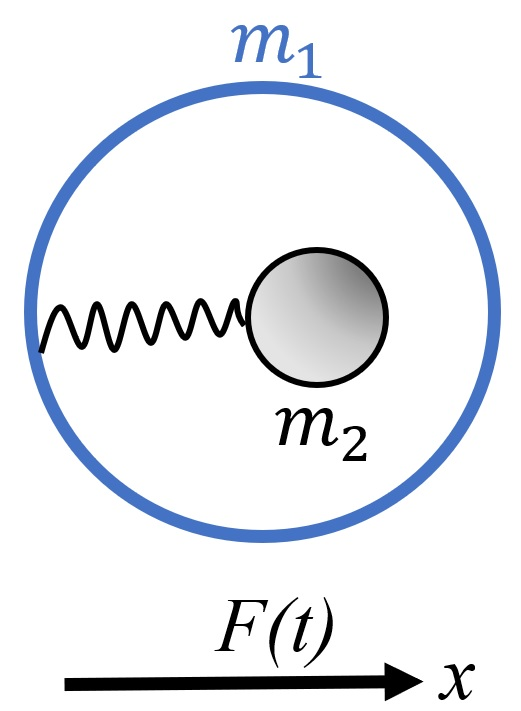
\includegraphics[height=1.05in,width=0.7in,viewport=0 0 380 550,clip]{Figures/A_mechanical_model_giving_rise_to_the_negative_effective_mass_effect.jpg}
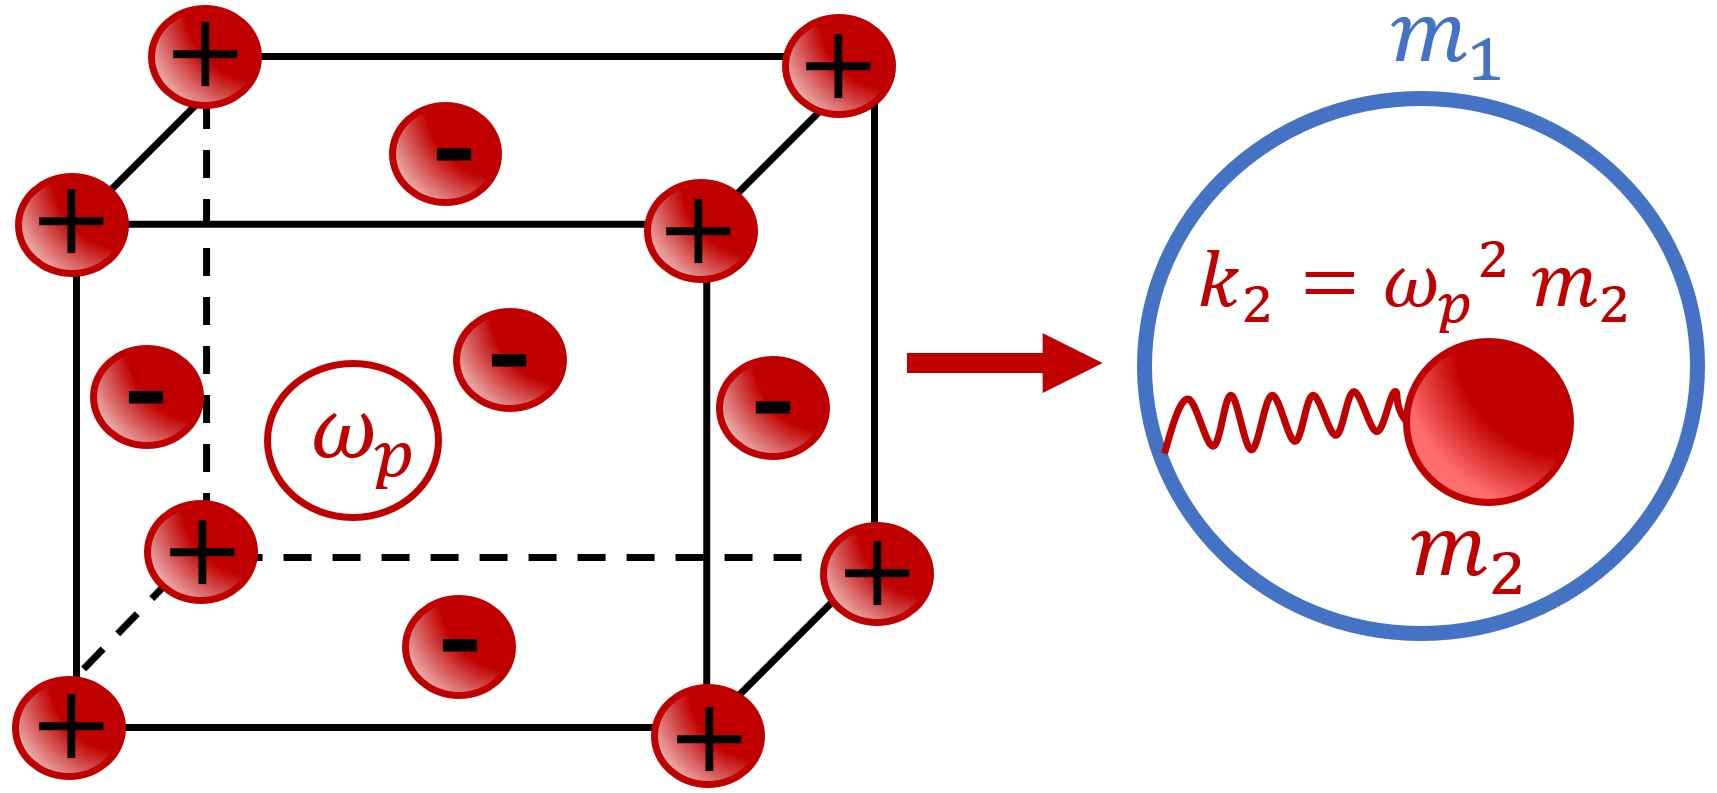
\includegraphics[height=1.55in,width=3.25in,viewport=0 0 1300 600,clip]{Figures/Equivalent_mechanical_scheme_of_electron_gas_in_ionic_lattice.jpg}
\caption{\fontsize{5.5pt}{4.2pt}\selectfont{\textrm{Equivalent mechanical scheme of electron gas in ionic lattice.}}}%
\label{Electron-gas-in-lattice}
\end{figure} 
			$\omega_{\mathrm{p}}$是载流子的等离振荡频率
			\begin{displaymath}
				\omega_{\mathrm{p}}^2=\frac{4\pi ne^2}m
			\end{displaymath}
}

\frame
{
	\frametitle{电场对导带电子的影响}
\begin{figure}[h!]
\centering
\vspace*{-13pt}
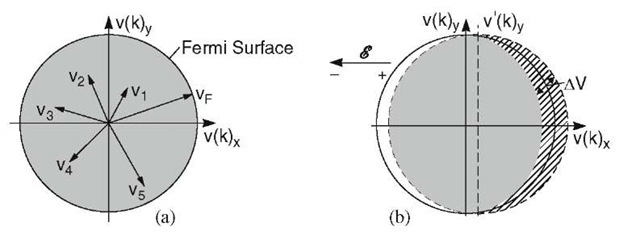
\includegraphics[height=1.4in,width=3.8in,viewport=0 0 480 180,clip]{Figures/Electrmagnetic_Fermi-surface-1.jpg}
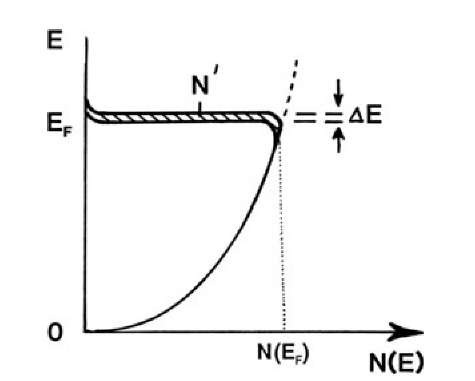
\includegraphics[height=1.35in,width=2.2in,viewport=0 0 200 130,clip]{Figures/Electrmagnetic_Fermi-surface-2.jpg}
\caption{\fontsize{5.5pt}{4.2pt}\selectfont{\textrm{Schematic representation of the Fermi-surface affected by the electrmagnetic field.}}}%
\label{CB-Electron-in-E}
\end{figure} 
}

\frame
{
	\frametitle{\textrm{Lorentz-Drude}模型}
\begin{itemize}
	\item \textrm{Lorentz-Model}:\\
		始于电子与晶格离子间作用,侧重描述电子在固体中的运动,介电函数为
		\begin{displaymath}
			\varepsilon(\omega)=1-\dfrac{\omega_{\mathrm{p}^2}}{\omega^2+\mathrm{i}\omega\tau-\omega_0^2}
		\end{displaymath}
		\textcolor{blue}{\textrm{Lorentz}模型中,取$\omega_0=0$,即为\textrm{Drude}模型}
	\item \textrm{Drude-Model}:\\
		侧重描述自由电子气对外部交变电场的响应,则介电函数可以表示为:
			\begin{displaymath}
				\varepsilon(\omega)=1-\frac{\omega_\mathrm{p}^2}{\omega(\omega+\mathrm{i}/\tau)}=\underline{\textcolor{blue}{\left[ 1-\frac{\omega_{\mathrm{p}}^2\tau^2}{1+\omega^2\tau^2} \right]}}+\mathrm{i}\underline{\textcolor{blue}{\left[ \frac{\omega_{\mathrm{p}}^2\tau}{\omega(1+\omega^2\tau^2)} \right]}}
			\end{displaymath}
%\begin{displaymath}
\end{itemize}
}

\frame
{
	\frametitle{\textrm{Lorentz-Drude}模型}
\begin{figure}[h!]
\centering
\vspace*{-13pt}
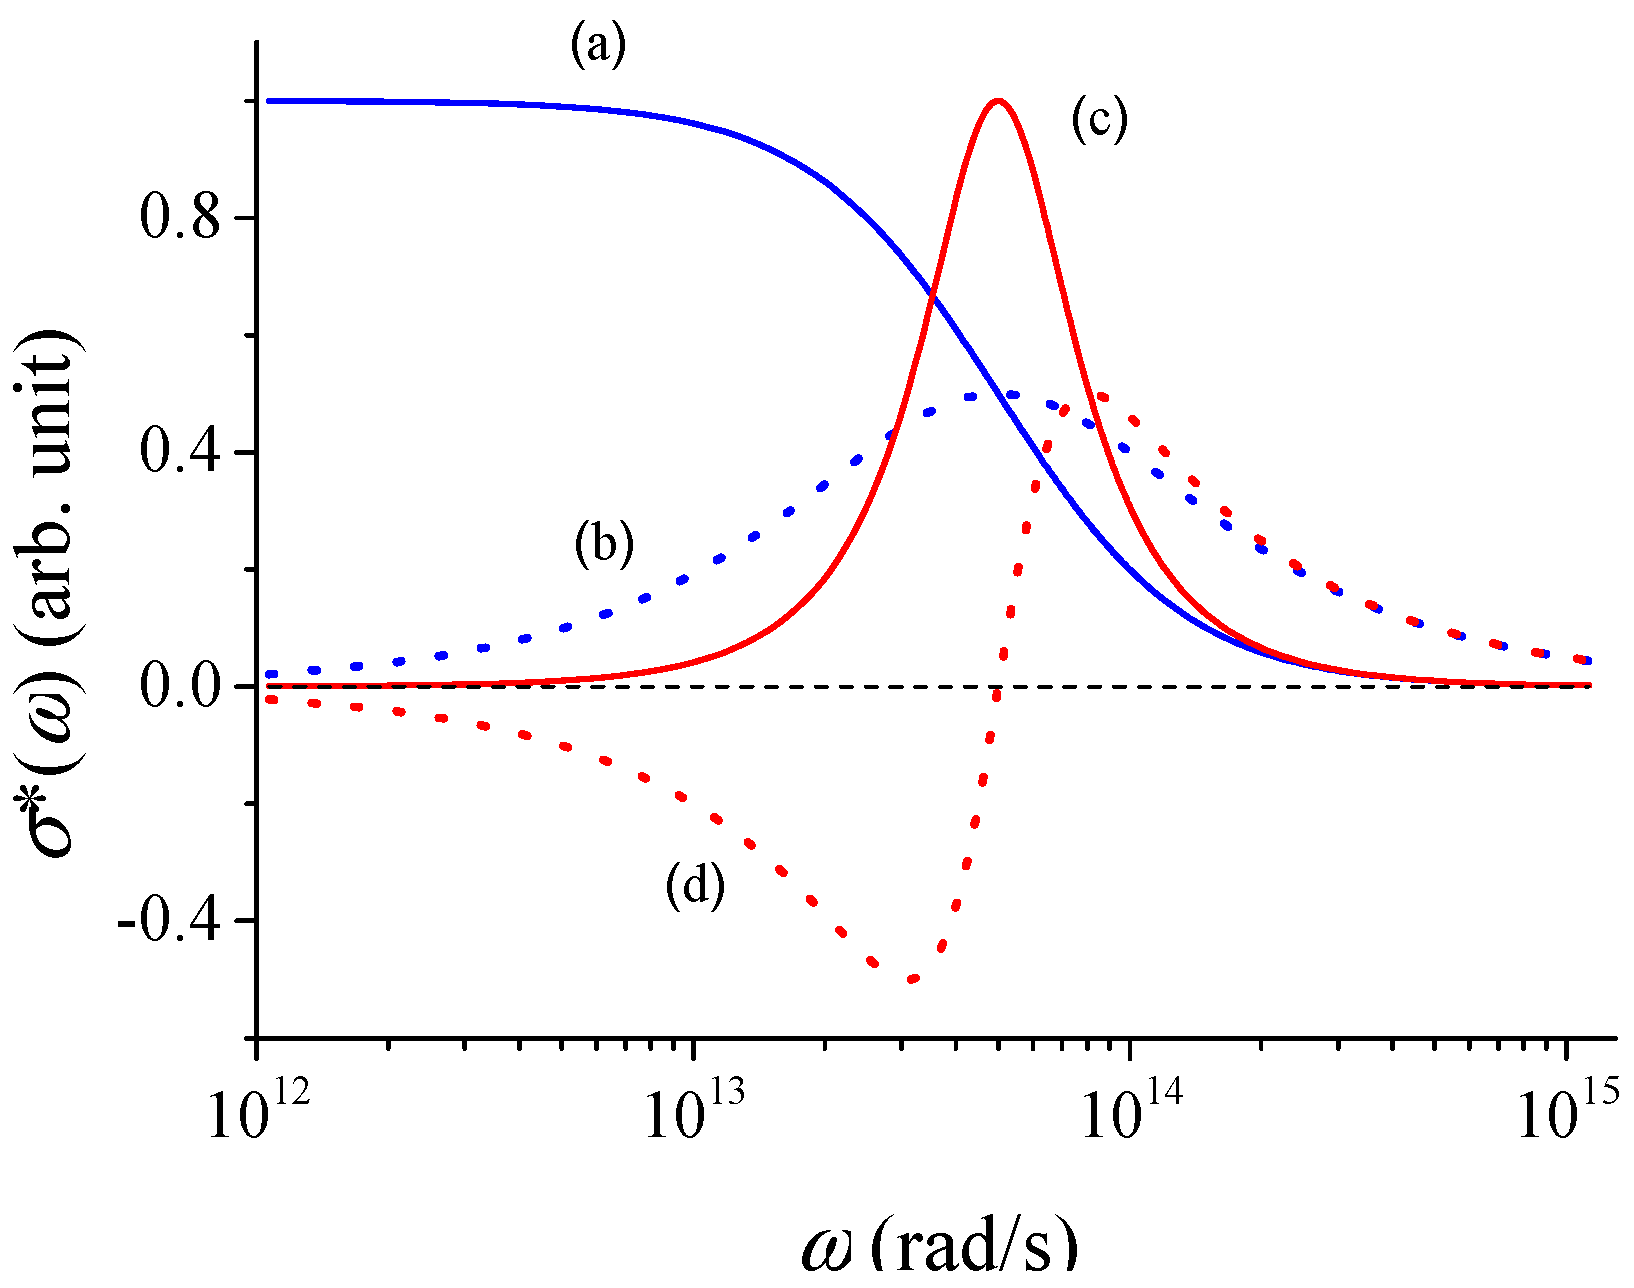
\includegraphics[height=2.5in,width=3.6in,viewport=0 0 200 155,clip]{Figures/Optical-conductivity-in-the-Drude-relaxation-and-in-the-Lorentz-resonance.png}
\caption{\fontsize{5.5pt}{4.2pt}\selectfont{\textrm{Optical conductivity in the Drude relaxation ((a) and (b)) and in the Lorentz resonance ((c) and (d)).}}}%
\label{Drude-vs-Lorentz}
\end{figure} 
}

\frame
{
	\frametitle{\textrm{Lorentz-Drude}模型}
\begin{figure}[h!]
\centering
\vspace*{-13pt}
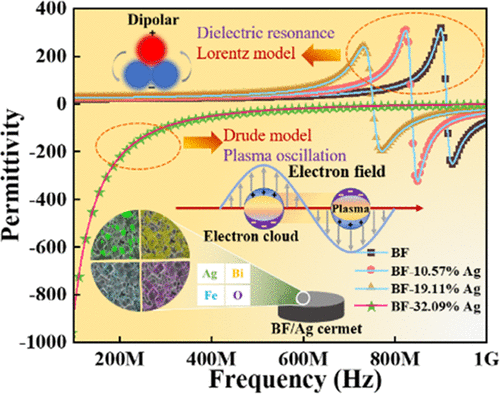
\includegraphics[height=2.7in,width=3.6in,viewport=0 0 500 400,clip]{Figures/Lorentz_Drude-model.png}
\caption{\fontsize{5.5pt}{4.2pt}\selectfont{\textrm{Optical permittivity in the Plasma oscillation and in the Dielectric resonance.}}}%
\label{Drude-vs-Lorentz}
\end{figure} 
}

\frame
{
	\frametitle{\textrm{Drude}模型}
	\textcolor{blue}{在远红外区,经典自由电子气模型可以很好地描述金属的光学行为}
	如果载流子密度为$n$,则电流密度
	\begin{displaymath}
		\mathbf{J}=n(-e)\dot{\vec r}=n(-e)(-\mathrm{i}\omega)\vec A_0\mathrm{e}^{-\mathrm{i}\omega t}=\frac{ne^2\tau}m\frac1{1-\mathrm{i}\omega\tau}\mathbf{E}_0\mathrm{e}^{-\mathrm{i}\omega t}
	\end{displaymath}
	由此可得频率有关的电导率表示为
	\begin{displaymath}
		\sigma(\omega)=\frac{ne^2\tau}m\frac1{1-\mathrm{i}\omega\tau}=\sigma_0\frac1{1-\mathrm{i}\omega\tau}
	\end{displaymath}
	其中$\sigma_0=ne^2\tau/m$是静态电导率
%	\begin{itemize}
%		\item 
	介电函数可表示为
	\begin{displaymath}
	\epsilon_1(\omega)=1-\frac{\omega_{\mathrm{p}}^2\tau^2}{1+\omega^2\tau^2}\quad \epsilon_2(\omega)=\frac{\omega_{\mathrm{p}}^2\tau}{\omega(1+\omega^2\tau^2)}\quad
\end{displaymath}
%	\end{itemize}
}

\subsection{带间电子的激发}
\frame
{
\frametitle{带间跃迁的计算}
\begin{itemize}
\setlength{\itemsep}{10pt}
	\item 用半经典方法处理周期性体系的光学性质,用量子力学处理介质,对电磁波仍然采用经典电动力学描写
	\item 以半导体中的带间垂直跃迁(价带$|v,\vec k\rangle$,导带$|c,\vec k\rangle$)为例讨论固体的能带间跃迁
\begin{figure}[h!]
\centering
%\hspace*{-10pt}
\vspace*{-0.2in}
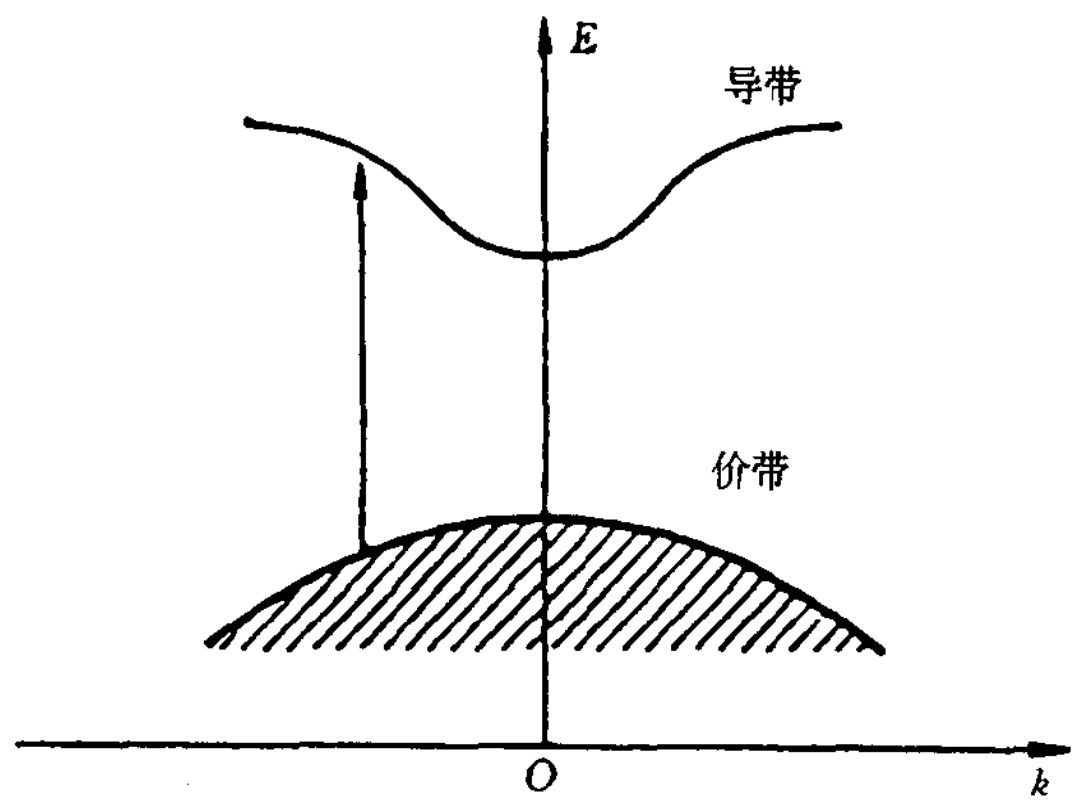
\includegraphics[height=1.8in,width=2.0in,viewport=0 0 1000 900,clip]{Figures/optic_dir.png}
\caption{\fontsize{8.0pt}{5.2pt}\selectfont\textrm{Schematic representation of directly inter-band transition.}}%
\label{Optic-dir}
\end{figure} 
\end{itemize}
}

\frame
{
	\frametitle{带间跃迁的计算}
%\begin{itemize}
	晶体中动量为$\vec p$的电子在电磁场(电磁场矢量势为$\mathbf{A}$)存在情况下,应用含时微扰理论,
\begin{displaymath}
	\hspace*{-10pt}
	H=\frac1{2m}[\vec p+\frac{e}c\mathbf{A}(\vec r,t)]^2+V(\vec r)=\left[ \frac{\vec p^2}{2m}+V(\vec r) \right]+\frac{e}{mc}\mathbf{A}\cdot\vec p+\frac{e^2}{2mc^2}\mathbf{A}^2
\end{displaymath}
其中电磁波
\begin{displaymath}
	\mathbf{A}(\vec r,t)=A_0\mathbf{e}\mathrm{e}^{\mathrm{i}(\vec q\cdot\vec r-\omega t)}+\mathrm{c.c}\quad\mathbf{e}\bot\vec q
\end{displaymath}
准确到$\vec A$的线性项(忽略$\vec A$的平方项)\textrm{Hamiltonian}为:
\begin{displaymath}
	H=\left[ \frac{\vec p^2}{2m}+V(\vec r) \right]+\frac{eA_0}{mc}\mathrm{e}^{\mathrm{i}(\vec q\cdot\vec r-\omega t)}\mathbf{e}\cdot\vec p+\frac{eA_0}{mc}\mathrm{e}^{-\mathrm{i}(\vec q\cdot\vec r-\omega t)}\mathbf{e}\cdot\vec p
\end{displaymath}
%	\item 
频率为$\omega$的平面偏振光,电场和磁场的强度为
\begin{displaymath}
%  \left\{
\begin{aligned}
	\vec E&=-\frac1c\frac{\partial\mathbf{A}}{\partial t}\\
	\vec B&=\nabla\times\mathbf{A}
  \end{aligned}%\right.
  \label{eq:optic-26}
\end{displaymath}
%\end{itemize}
%式中$c$为光速。
}

\frame
{
\frametitle{带间跃迁的计算}
在含时微扰\textrm{Hamiltonian}作用下,带间垂直跃迁为
\begin{displaymath}
	\begin{aligned}
		W(\vec q,\omega)=&\frac{2\pi}{\hbar}\left( \frac{eA_0}{m_ec} \right)^22\sum_{i,j}|\langle c,\vec k|\mathrm{e}^{\mathrm{i}\vec q\cdot\vec r}\mathbf{e}\cdot\vec p|v,\vec k\rangle|^2\\
		\times&\delta[E_c(\vec k)-E_v(\vec k)-\omega][f(E_c(\vec k))-f(E_v(\vec k))]
	\end{aligned}
  \label{eq:optic-27}
\end{displaymath}
$\delta$因子表示跃迁过程的能量守恒关系%,矩阵元$\langle c\vec k|H'|v\vec k\rangle$表示\textrm{Bloch}函数间的积分
。对垂直跃迁,忽略磁场贡献,%矩阵元可以简写成$\dfrac1cA_0\vec e\cdot\vec M_{cv}(\vec k)$,$\vec s$为电磁波矢量势$\vec A_0(=A_0\vec s)$方向的单位矢量。
只有满足能量守恒和动量守恒条件的跃迁才对积分有贡献。%$\displaystyle\int W\dfrac{\textrm{d}\vec k}{(2\pi)^3}$为单位体积、单位时间内吸收能量为$\omega$的光子的总数,系数2是考虑两种自旋态。将式\eqref{eq:optic-27},\eqref{eq:optic-28}代入式\eqref{eq:optic-29},并应用$\dfrac{A_0}c\vec e\cdot\vec M_{cv}(\vec k)$表示矩阵元,得

电磁波在介质中产生的电场
\begin{displaymath}
	\mathbf{E}(\vec r,t)=-\frac1c\frac{\partial\mathbf{A}}{\partial t}=E_0\mathbf{e}\mathrm{e}^{\mathrm{i}\vec q\cdot\vec r-\omega t}+\mathrm{c.c}\quad\mbox{其中}E_0=\mathrm{i}\omega\frac{A_0}c
\end{displaymath}

介质中的传导电流
\begin{displaymath}
	\mathbf{J}(\vec r,t)=\sigma(\vec q,\omega)E_0\mathbf{e}\mathrm{e}^{\mathrm{i}(\vec q\cdot\vec r-\omega t)}+\mathrm{c.c}\quad(\mathbf{e}\bot\vec q)
\end{displaymath}
由此计算得到吸收功率
\begin{displaymath}
	\int_V\mathbf{J}\cdot\mathbf{E}\mathrm{d}\vec r=2\sigma_1(\vec q,\omega)|E_0|^2V=2\sigma_1(\vec q,\omega)\frac1{c^2}\omega^2A_0^2V=\textcolor{blue}{\hbar\omega W(\vec q,\omega)}
\end{displaymath}
}

\frame
{
	\frametitle{带间跃迁的计算}
长波极限下($\vec q\rightarrow0$), 根据光学性质的基本关系,可有介电函数的介电函数虚部表达式
\begin{displaymath}
	\begin{aligned}
		\varepsilon_2(\omega)=&\lim_{\vec q\rightarrow0}\frac{8\pi^2e^2}{m_e^2\omega^2}\int\frac{\mathrm{d}\vec k}{(2\pi)^3}|\langle c,\vec k|\mathbf{e}\cdot\vec p|v,\vec k\rangle|^2\\
		\times&\delta(E_c(\vec k)-E_v(\vec k)-\hbar\omega)[f(E_c(\vec k))-f(E_v(\vec k))]
	\end{aligned}
  \label{eq:optic-varepsilon_2}
\end{displaymath}
$\varepsilon_2(\omega)$是晶体的光学吸收和能带结构之间的基本关系

对应的$\varepsilon_1$可以根据\textrm{Kramers-Kr\"onig}关系%\eqref{eq:optic-16}
得到
\begin{displaymath}
	\varepsilon_1(\omega)=1+\frac1{\pi}\mathscr{P}\int_{-\infty}^{+\infty}\frac{\varepsilon_2(\omega^{\prime})}{\omega^{\prime}-\omega}\textrm{d}\omega^{\prime}=1+\frac2{\pi}\mathscr{P}\int_0^{+\infty}\frac{\omega^{\prime}\varepsilon_2(\omega^{\prime})}{\omega^{\prime2}-\omega^2}\textrm{d}\omega^{\prime}
  \label{eq:optic-varepsilon_1}
\end{displaymath}
因此介电函数表示为
\begin{displaymath}
	\hspace*{-10pt}
	\varepsilon(\omega)=1+\frac{8\pi e^2}{m_e^2}\int\frac{\mathrm{d}\vec k}{(2\pi)^3}\frac{|\langle c,\vec k|\mathbf{e}\cdot\vec p|v,\vec k\rangle|^2}{(E_c(\vec k)-E_v(\vec k))/\hbar^2}\frac{(-\mathrm{i})[f(E_c(\vec k))-f(E_v(\vec k))]}{E_c(\vec k)-E_v(\vec k)-\hbar\omega-\mathrm{i}\eta}
  \label{eq:optic-varepsilon}
\end{displaymath}
}

\frame
{
	\frametitle{带间跃迁和带内跃迁的计算}
电导率函数可表示为
\begin{displaymath}
	\sigma(\omega)=\frac{2e^2}{m_e^2}\int\frac{\mathrm{d}\vec k}{(2\pi)^3}\frac{|\langle c,\vec k|\mathbf{e}\cdot\vec p|v,\vec k\rangle|^2}{(E_c(\vec k)-E_v(\vec k))/\hbar}\frac{(-\mathrm{i})[f(E_c(\vec k))-f(E_v(\vec k))]}{E_c(\vec k)-E_v(\vec k)-\hbar\omega-\mathrm{i}\eta}
  \label{eq:optic-sigma}
\end{displaymath}

\textcolor{violet}{推广到长波极限下的带内跃迁}
\begin{displaymath}
	f(E_c(\vec k))-f(E_v(\vec k))\approx\frac{\partial f}{\partial E}(f(E_c(\vec k))-f(E_v(\vec k)))
\end{displaymath}
\begin{displaymath}
	\sigma(\omega)=\frac{e^2\hbar}{4\pi^3}\int\mathrm{d}\vec k\langle c,\vec k|\mathbf{e}\cdot\vec p|v,\vec k\rangle|^2\frac{-\mathrm{i}}{E_c(\vec k)-E_v(\vec k)-\hbar\omega-\mathrm{i}\eta}\left( -\frac{\partial f}{\partial E} \right)
\end{displaymath}
引入等式$\eta=\hbar/\tau$,并作展开
\begin{displaymath}
	E_{\vec k+\vec q}-E_{\vec k}\approx\vec q\cdot(\partial E/\partial\vec k)=\frac{\hbar}{m_e}\langle c,\vec k|\mathbf{q}\cdot\vec p|v,\vec k\rangle
\end{displaymath}
由此可得
\vspace{-5pt}
\begin{displaymath}
	\sigma(\vec q,\omega)=\frac{e^2}{4\pi^3}\int\mathrm{d}\vec k\frac{\tau|\langle c,\vec k|\mathbf{e}\cdot\vec p|v,\vec k\rangle|^2}{1-\mathrm{i}\tau(\omega-\langle c,\vec k|\mathbf{q}\cdot\vec p|v,\vec k\rangle)}\left( -\frac{\partial f}{\partial E} \right)
\end{displaymath}
}

\frame
{
	\frametitle{联合态密度\textrm{(Joint DOS, JDOS)}}
定义联合态密度(\textrm{Joint Density of States, JDOS})
\begin{displaymath}
  J_{cv}(\hbar\omega)=\sum_{v,c}\int\delta[E_c(\vec k)-E_v(\vec k)-\omega]\frac{2\textrm{d}\vec k}{(2\pi)^3}
  \label{eq:optic-33}
\end{displaymath}
令$E_{cv}(\vec k)$\,=\,$E_c(\vec k)-E_v(\vec k)$,因$\textrm{d}\vec k$\,=\,$\dfrac{dE_{cv}(\vec k)}{\nabla_{\vec k}E_{cv}(\vec k)}\textrm{d}S$,故有
\begin{displaymath}
  J_{cv}(\omega)=\frac2{(2\pi)^3}\sum_{v,c}\int\limits_{E_{cv}(\vec k)=\omega}\frac{\textrm{d}S}{\nabla_{\vec k}E_{cv}(\vec k)}
  \label{eq:optic-34}
\end{displaymath}
类似态密度的定义,而$E_{cv}(\vec k)$同时联系着价带和导带,因此称为联合态密度。当矩阵元$\vec M_{cv}(\vec k)$随波矢$\vec k$变化比较小的时候,可以近似地认为$\varepsilon_2(\omega)\!\propto\!J_{cv}(\omega)$。满足$|\nabla_{\vec k}E_{cv}(\vec k)|\!=\!0$的$\vec k$点,是联合态密度$J_{cv}(\omega)$和$\varepsilon_2(\omega)$的奇点(\textrm{Van Hove}奇点或临界点),在这些点,$J_{cv}(\omega)$和$\varepsilon_2(\omega)$%的能谱图将出现典型结构(即
对能量的微商呈现典型的不连续。%联合态密度的奇点有两种情况,即$\nabla_{\vec k}E_c(\vec k)\!=\!\nabla_{\vec k}E_v(\vec k)\!=\!0$和$\nabla_{\vec k}E_c(\vec k)\!=\!\nabla_{\vec k}E_v(\vec k)\!\neq\!0$。将$E_{cv}(\vec k)$在奇点作Taylor级数展开到二级,$$E_{cv}(\vec k)=E_0+a_xk_x^2+a_yk_y^2+a_zk_z^2$$可以看出有四种类型的奇点:
}

\frame
{
	\frametitle{联合态密度\textrm{(Joint DOS, JDOS)}}
\begin{figure}[h!]
\centering
%\hspace*{-10pt}
\vspace*{-0.05in}
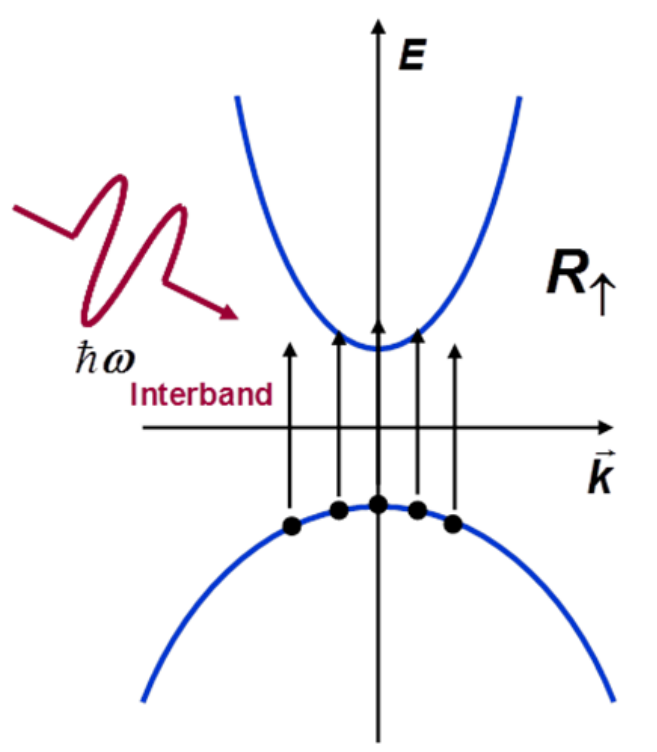
\includegraphics[height=2.0in,width=1.7in,viewport=0 0 630 760,clip]{Figures/Inter_band-transition_R.png}
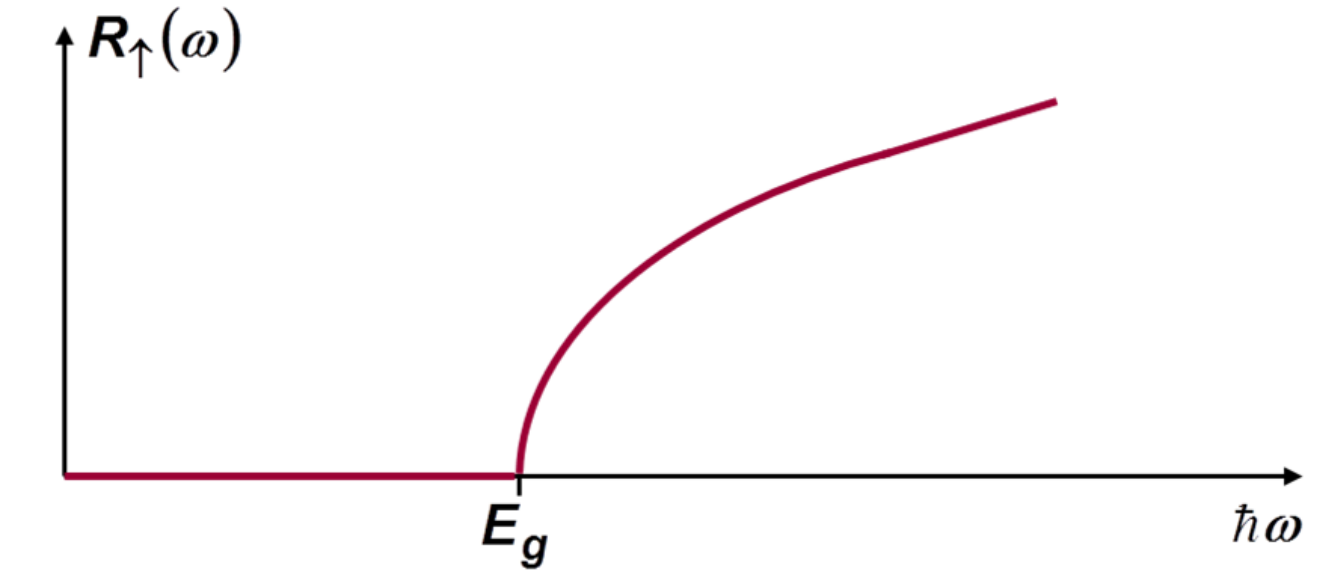
\includegraphics[height=1.0in,width=2.15in,viewport=0 0 1320 580,clip]{Figures/Inter_band-transition_JDOS.png}
\caption{\fontsize{5.2pt}{4.0pt}\selectfont\textrm{Schematic representation of the joint-DOS and the Van-Hove singularity.}}%
\label{Optic-JDOS}
\end{figure} 
}

\subsection{复杂的光子与电子相互作用}
\frame
{
	\frametitle{电子对光子的吸收与受激辐射}
电子、空穴与相互作用	
\begin{figure}[h!]
\centering
%\hspace*{-10pt}
\vspace*{-0.2in}
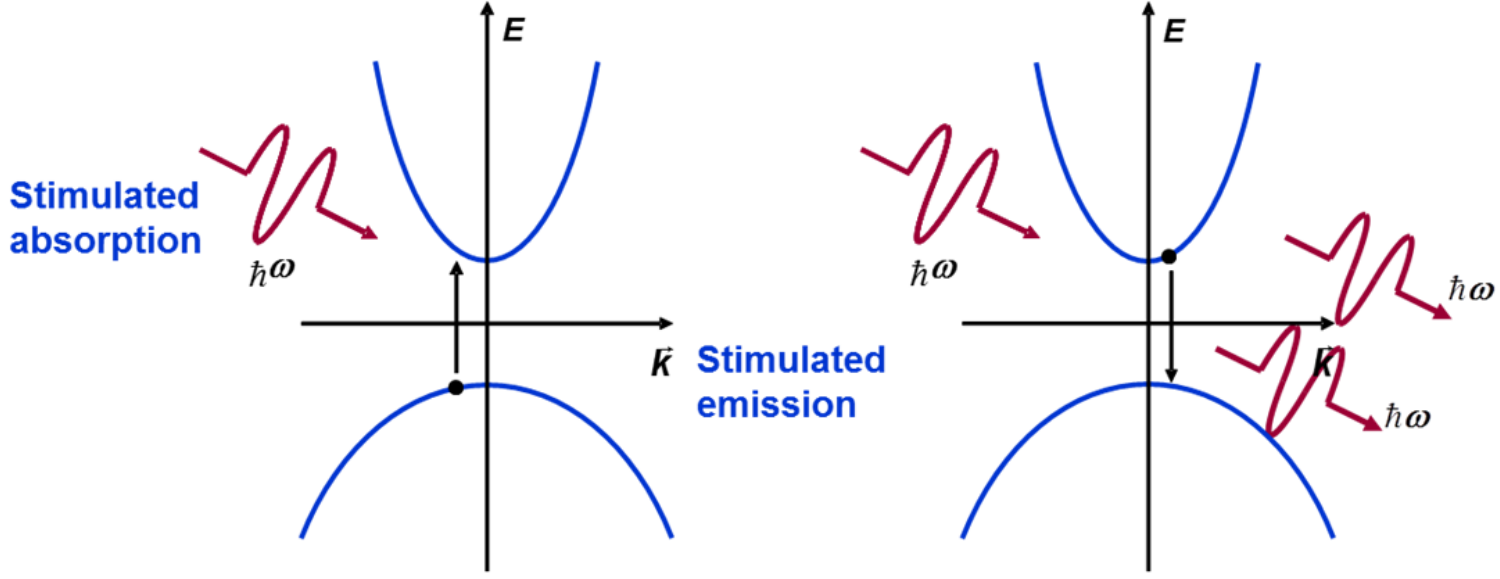
\includegraphics[height=1.9in,width=4.1in,viewport=0 0 1500 600,clip]{Figures/Inter_band-transition_abs-emi.png}
\caption{\fontsize{5.2pt}{4.0pt}\selectfont\textrm{Schematic representation of the stimulated absorption and emission of electrons.}}%
\label{Stimulated-absorption-emission}
\end{figure} 
电子-空穴对构成准粒子\textrm{(quasi-particle)}
}

\frame
{
	\frametitle{电子的自发辐射}
	电子-空穴的复合与准粒子的寿命
\begin{figure}[h!]
\centering
%\hspace*{-10pt}
\vspace*{-0.05in}
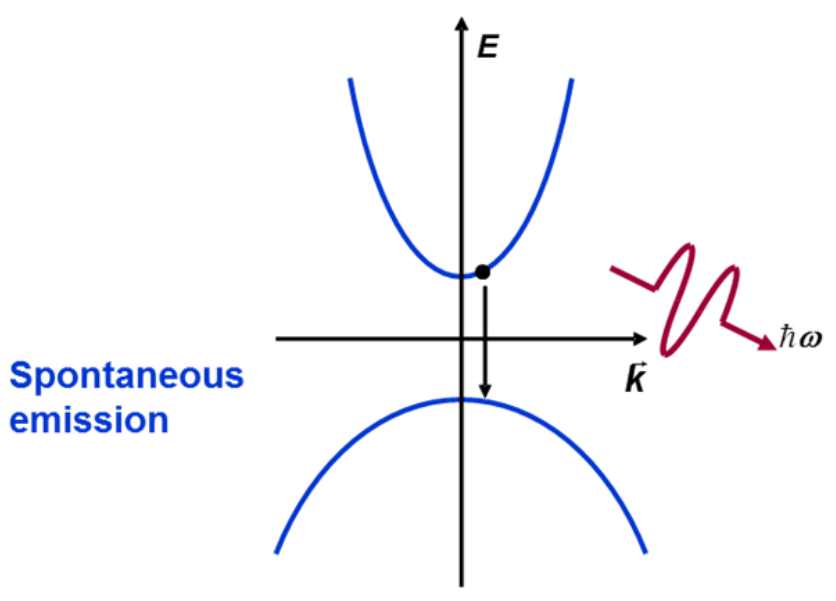
\includegraphics[height=2.0in,width=2.7in,viewport=0 0 830 620,clip]{Figures/Inter_band-transition_emission.png}
\caption{\fontsize{5.2pt}{4.0pt}\selectfont\textrm{Schematic representation of the spontaneous emission of electrons.}}%
\label{spontaneous-emission}
\end{figure} 
}

\frame
{
	\frametitle{复杂的系间窜越:~荧光、磷光与内转换}
\begin{figure}[h!]
\centering
%\hspace*{-10pt}
\vspace*{-0.05in}
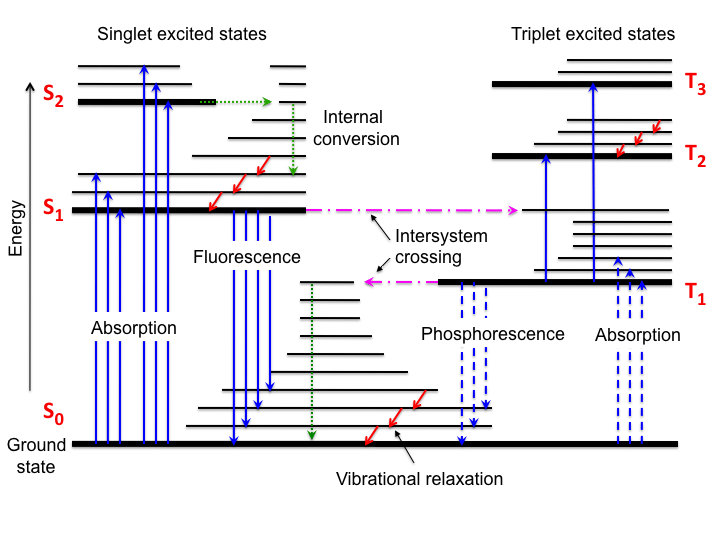
\includegraphics[height=2.3in,width=3.3in,viewport=0 0 720 520,clip]{Figures/Typical-diagram-of-the-electronic-energy-levels-of-a-molecule-with-singlet-and-triplet.png}
\caption{\fontsize{5.2pt}{4.0pt}\selectfont\textrm{Typical diagram of the electronic energy levels of a molecule with singlet and triplet  systems. The most important radiative (fluorescence and phosphorescence) and non-radiative (internal conversion, vibrational relaxation, intersystem crossing) transitions are shown.}}%
\label{singlet-triplet}
\end{figure} 
}

\frame
{
	\frametitle{吸收谱与发射谱}
\begin{figure}[h!]
\centering
%\hspace*{-10pt}
\vspace*{-0.19in}
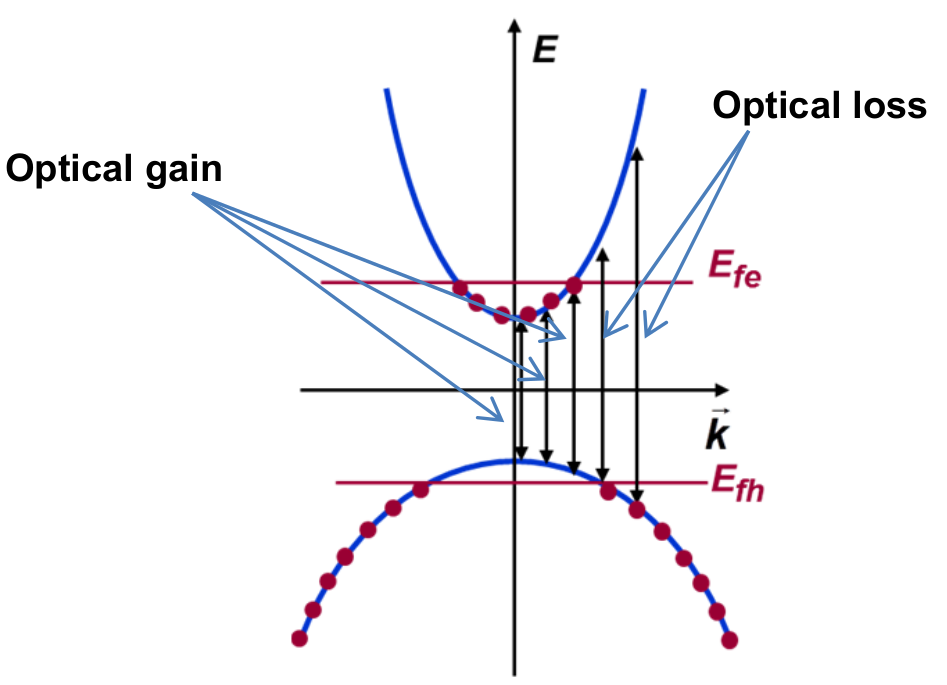
\includegraphics[height=2.5in,width=3.80in,viewport=0 0 950 700,clip]{Figures/Optical_gain-loss.png}
%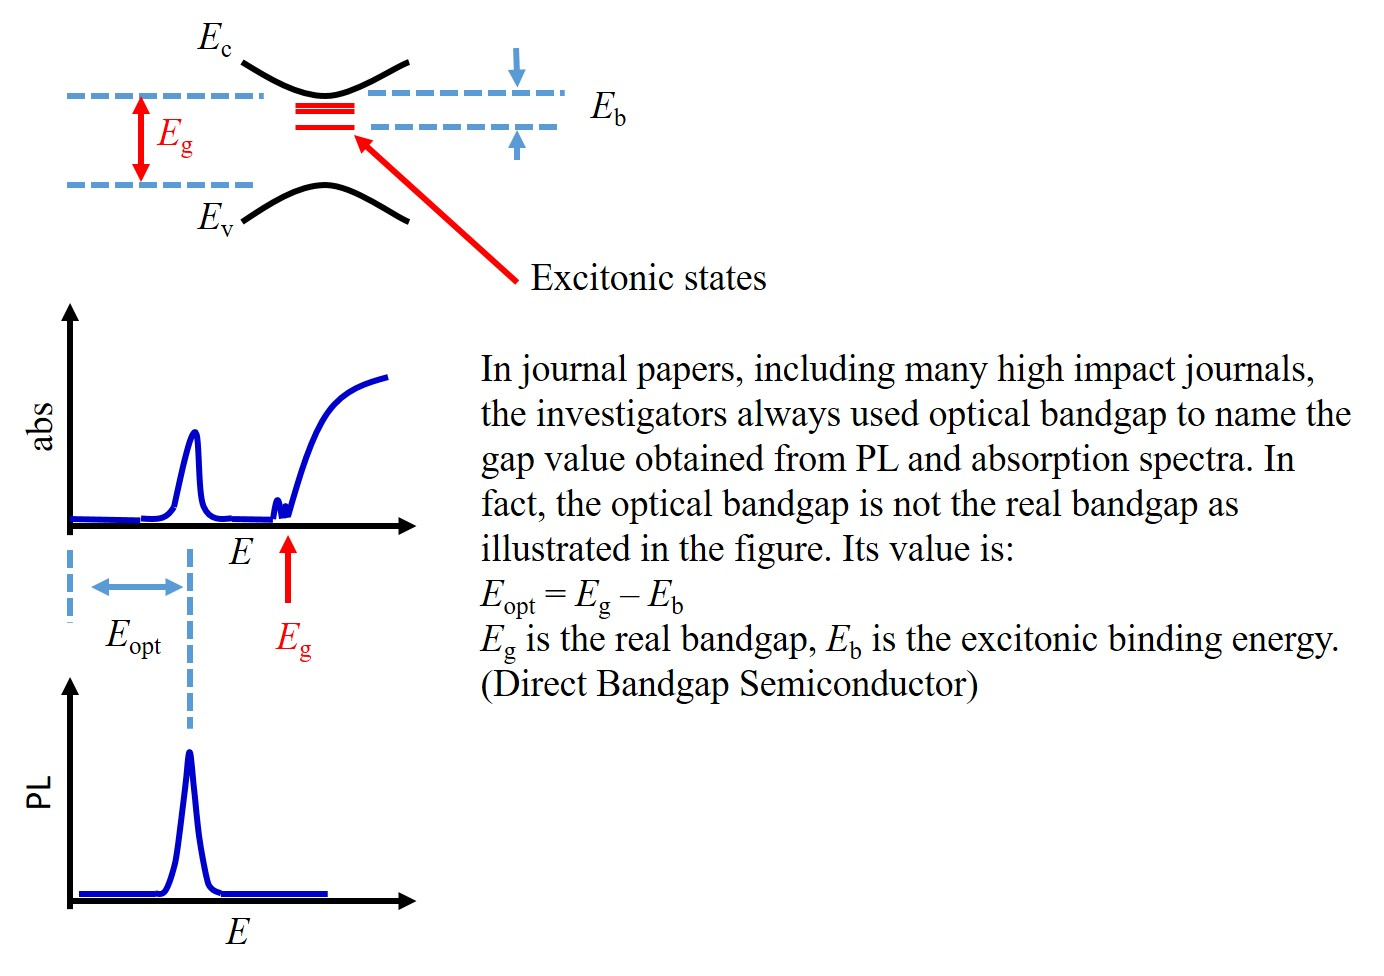
\includegraphics[height=1.1in,width=2.00in,viewport=0 0 670 460,clip]{Figures/Optical_Bandgap.jpg}
\caption{\fontsize{5.2pt}{4.0pt}\selectfont\textrm{Schematic representation of the gain-loss spectra.}}%
\label{gain-loss_Bandgap}
\end{figure} 
}

\frame
{
	\frametitle{光电子能谱与电子带隙}
\begin{figure}[h!]
\centering
%\hspace*{-10pt}
\vspace*{-3pt}
%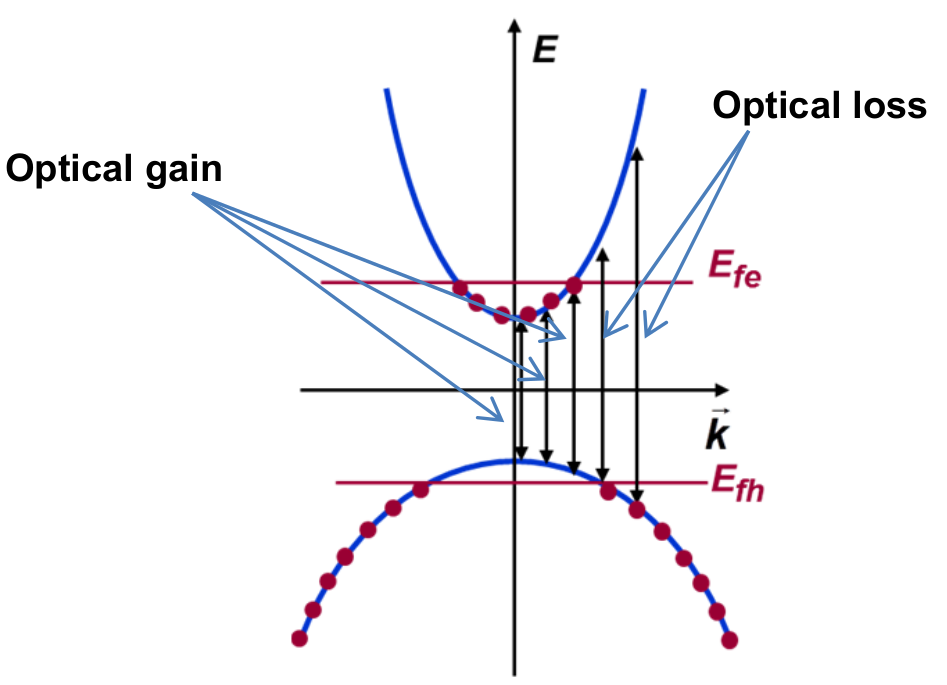
\includegraphics[height=1.7in,width=2.30in,viewport=0 0 950 700,clip]{Figures/Optical_gain-loss.png}
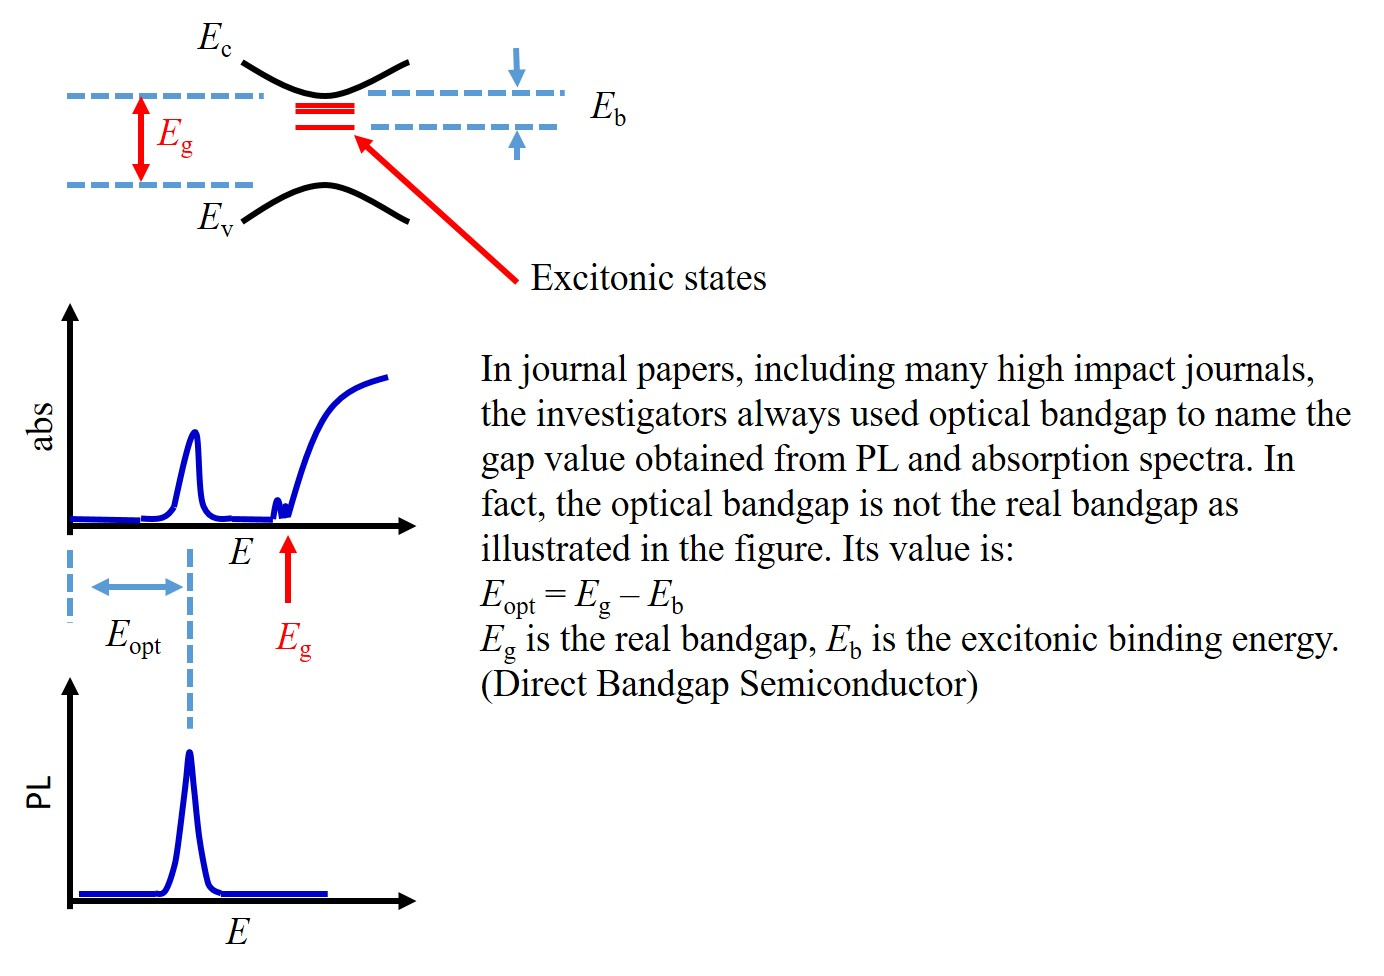
\includegraphics[height=2.4in,width=4.00in,viewport=0 0 670 460,clip]{Figures/Optical_Bandgap.jpg}
\caption{\fontsize{5.2pt}{4.0pt}\selectfont\textrm{Schematic representation of the spectra vs the band gap.}}%
\label{gain-loss_Bandgap}
\end{figure} 
}
\section{晶格振动与分子动力学}
\frame
{
	\frametitle{原子间相互作用力的表示}
	分子动力学模拟中影响结果最主要因素之一是\textcolor{purple}{原子间相互作用力}的准确度
\vskip 5pt
\begin{itemize}
	\item 经典分子动力学模拟中,原子间相互作用力是根据经验势函数得到的\footnote{\fontsize{6.2pt}{4.2pt}\selectfont{经验势函数也称为力场,是参数化形式给出的原子间相互作用,一般通过对实验数据拟合或小体系的第一原理计算得到}}。构建一套高精度的经验势函数代价很高,而且经验势函数一般不具备可移植性
\end{itemize}
\vskip 5pt
	当动力学过程必须考虑量子效应(如电子影响的贡献不可忽略时),必须采用第一原理分子动力学\textrm{(Ab initio~MD,~AIMD)}
	\begin{itemize}
		\item 所谓第一原理分子动力学,就是在计算原子运动时,将电子结构变化的贡献考虑进来,因此在每一时间步长,体系实时构型下的原子受力计算,都必须伴随电子结构计算
	\end{itemize}
	一般电子结构计算采用\textrm{DFT}计算,不难想见,第一原理分子动力学模拟的代价极高
}

\subsection{晶格振动与简谐振动}
\frame
{
	\frametitle{晶格振动}
		晶体中的格点表示原子的平衡位置,晶格振动是原子在格点附近的振动
\begin{figure}[h!]
\centering
%\hspace*{-10pt}
\vspace*{-0.1in}
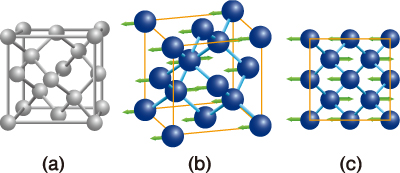
\includegraphics[height=1.9in,width=4.0in,viewport=0 0 400 185,clip]{Figures/Schematic-diagrams-of-the-crystal-structures-and-longitudinal-optical-lattice-vibration-modes-(LO_modes)-of-diamonds.jpg}
\caption{\tiny \textrm{Schematic diagrams of the crystal structures and longitudinal optical lattice vibration modes (LO modes) of diamonds. (a) Crystal structure of a diamond. (b) 3D view of a LO mode. (c) Top view of a LO mode.}}%
\label{lattice-virbration}
\end{figure} 
}

\frame
{
	\frametitle{简谐近似}
	\begin{itemize}
		\item 红外、\textrm{Raman}光谱、中子衍射谱,热容、热导,电阻、超导和电-声耦合等都与晶格振动有关
		\item 绝热近似%(\textrm{Born-Oppenheimer}近似)
			下,原子核是在电子能量函数$E(\mathbf{R})$构成的势能面上运动
	\end{itemize}
	含有$N$个原子,平衡位置是$\mathbf{R}_i^0$,偏移位置矢量$\mathbf{\mu}_i(t)$,体系的势能函数在平衡位置作\textrm{Taylor~}级数展开
	\begin{displaymath}
%		\begin{aligned}
		V=V_0+\sum_{i=1}^{3N}\left( \frac{\partial V}{\partial \mu_i} \right)_0\mu_i+\underline{\textcolor{red}{\frac12\sum_{i,j=1}^{3N}\left( \frac{\partial^2V}{\partial\mu_i\partial\mu_j} \right)_0\mu_i\mu_j}}+\mbox{高阶项}
%		\end{aligned}
	\end{displaymath}
	平衡位置$\left( \frac{\partial V}{\partial\mu_i} \right)_0=0$\\
	\textcolor{blue}{简谐近似}保留到$\mu_i$的二次项\\
	引入高阶项,则势函数可以包括\textcolor{purple}{非简谐近似}的贡献
}

\frame
{
	\frametitle{简谐振动与简正坐标}
	$N$原子体系的动能函数
	\begin{displaymath}
		T=\frac12\sum_{i=1}^{3N}m_i\dot{\mu}_i^2
	\end{displaymath}
	引入简正坐标,\textcolor{blue}{与原子位移坐标$\mu_i$正交变换}
	\begin{displaymath}
		\sqrt{m_i}\mu_i=\sum_{j=1}^{3N}a_{ij}Q_j
	\end{displaymath}
	\textcolor{red}{目的}:~系统的势能函数与动能函数有简单形式(只有平方项)
	\begin{displaymath}
%		\begin{aligned}
			T=\frac12\sum_{i=1}^{3N}\dot{Q}_i^2\quad
			V=\frac12\sum_{i=1}^{3N}\omega_i^2Q_i^2
%		\end{aligned}
	\end{displaymath}
	由此可得谐振方程
	\begin{displaymath}
		\ddot{Q}_i+\omega_i^2Q_i=0\quad i=1,2,3,\cdots,3N
	\end{displaymath}

}

\frame
{
	\frametitle{简谐振动与振动模式}
	任意简正坐标解
	\begin{displaymath}
		Q_i=A\sin(\omega_it+\delta)
	\end{displaymath}
	由此得到原子位移坐标
	\begin{displaymath}
		\mu_i=\frac{a_{ij}}{\sqrt{m_i}}A\sin(\omega_it+\delta)
	\end{displaymath}
\begin{figure}[h!]
\centering
%\hspace*{-10pt}
\vspace*{-0.1in}
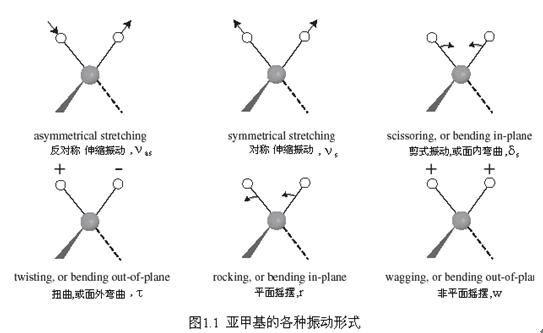
\includegraphics[height=1.in,width=2.in,viewport=0 20 420 250,clip]{Figures/RF_vir.jpg}
\caption{\tiny \textrm{Schematic example of vibration model of dimethyl.}}%
\label{virbration_model}
\end{figure} 
\textcolor{red}{简谐振动不表示某个原子的振动,表示整个体系所有原子参与的振动。这种体系中所有原子一起参加的集体运动常称为振动模}
}

\frame
{
	\frametitle{简谐振动与振动模式}
\begin{figure}[h!]
\centering
%\hspace*{-10pt}
\vspace*{-0.05in}
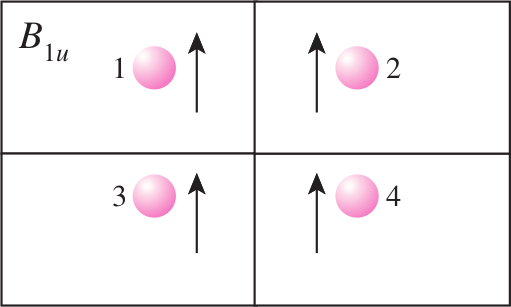
\includegraphics[height=1.1in,width=1.95in,viewport=0 0 520 310,clip]{Figures/Viberation_of_B1u.png}
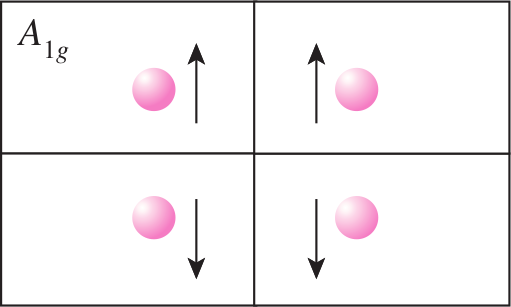
\includegraphics[height=1.1in,width=1.95in,viewport=0 0 515 310,clip]{Figures/Viberation_of_A1g.png}
\vskip 4pt
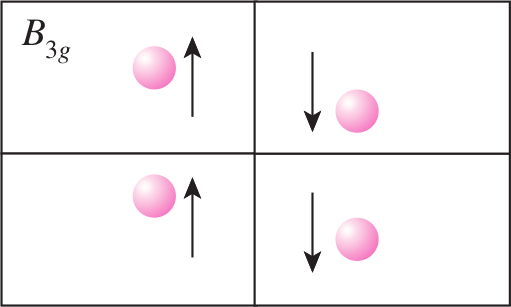
\includegraphics[height=1.1in,width=1.95in,viewport=0 0 520 310,clip]{Figures/Viberation_of_B3g.png}
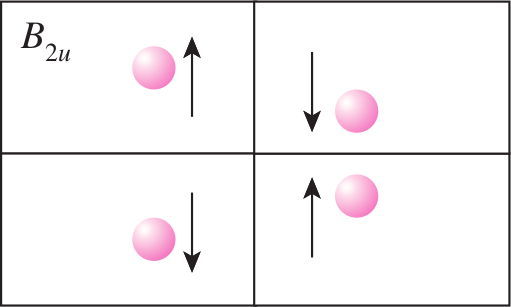
\includegraphics[height=1.1in,width=1.95in,viewport=0 0 515 310,clip]{Figures/Viberation_of_B2u.png}
\caption{\tiny \textrm{Schematic example of the symmetry of vibration model.}}%
\label{virbration_model-symmetry}
\end{figure} 
}

\frame
{
	\frametitle{一维单原子链}
\begin{figure}[h!]
\centering
%\hspace*{-10pt}
\vspace*{-0.25in}
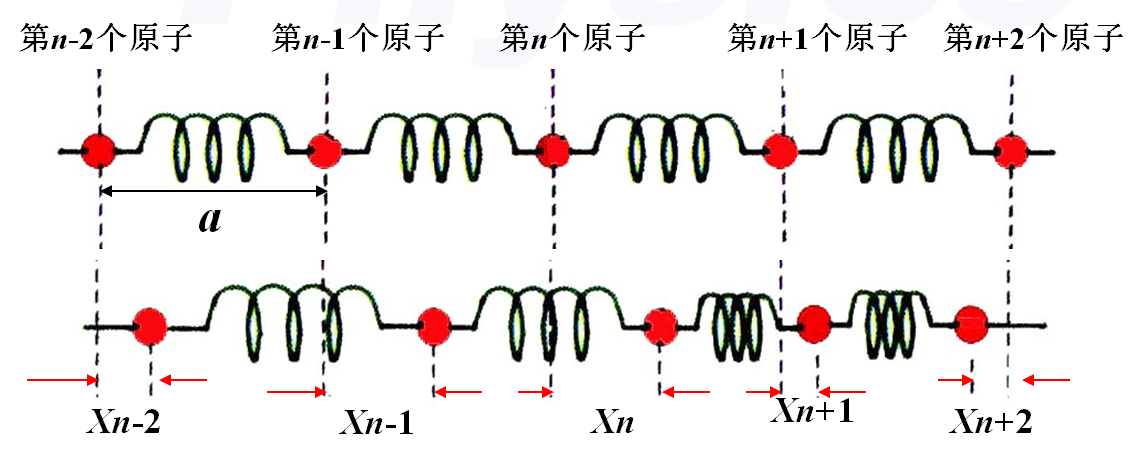
\includegraphics[height=1.0in,width=2.8in,viewport=0 0 1400 500,clip]{Figures/virbration.png}
\caption{\tiny \textrm{Schematic example of vibration of 1D-atomic chain.}}%
\label{virbration}
\end{figure} 
单原子链可以视为最简单的晶格,平衡时相邻原子距离为$\mathbf{a}$,原子限制在沿链方向运动,偏离格点位置用$\cdots,\mathbf{X}_{n-1},\mathbf{X}_{n},\mathbf{X}_{n+1},\cdots$,原子的振动可以表示为
\begin{displaymath}
	\mu_{nq}=A\mathrm{e}^{\mathrm{i}(\omega t-qx)}
\end{displaymath}
其中振幅$A$是常数,$\omega$是圆频率,$q=\tfrac{2\pi}{\lambda}$是波数,$\lambda$是波长
\vskip 5pt
\textcolor{blue}{根据量子理论,每种简谐振动的能量是量子化的,可以用声子表示}
\begin{displaymath}
	\varepsilon_{nq}=\left( n+\frac12 \right)\hbar\omega_q
\end{displaymath}
}

\frame
{
	\frametitle{谐振子模型}
\begin{figure}[h!]
\centering
%\hspace*{-10pt}
\vspace*{-0.15in}
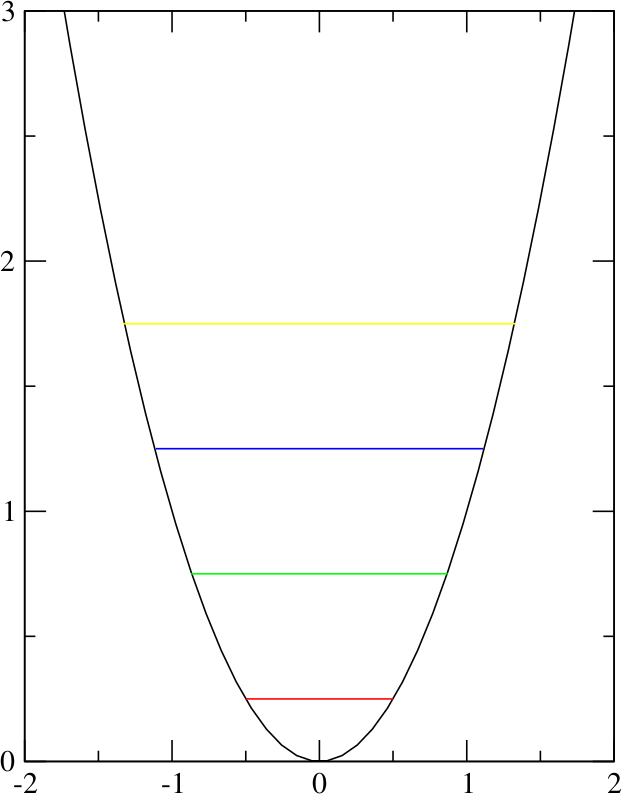
\includegraphics[height=2.7in,width=2.9in,viewport=0 0 650 800,clip]{Figures/Quantum-viberation.png}
\caption{\tiny \textrm{Schematic example of quantization of  harmonic oscillator model.}}%
\label{Harmonic-oscillator-model}
\end{figure} 
}

\frame
{
	\frametitle{双原子链与光学支和声学支}
\begin{figure}[h!]
\centering
%\hspace*{-10pt}
\vspace*{-0.20in}
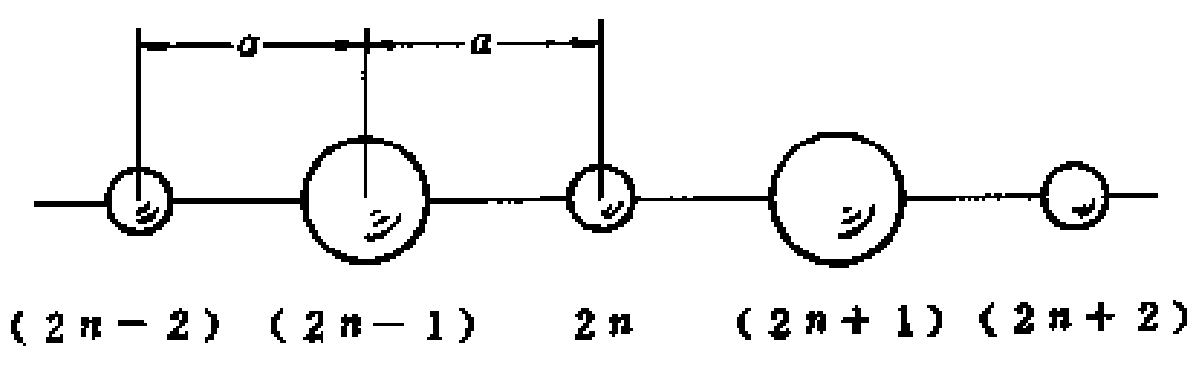
\includegraphics[height=0.7in,width=2.6in,viewport=0 0 1400 400,clip]{Figures/virbration-2.png}
\caption{\tiny \textrm{Schematic example of vibration of 1D-diatomic chain.}}%
\label{virbration-2D}
\end{figure} 
一维双原子链是最简单的复式晶格,平衡时相邻原子间距为$\mathbf{a}$,每个原胞含有两个不同原子\textrm{P}和\textrm{Q},质量分别是$m$和$M$,原子现在在沿链方向运动,偏离位移用$\cdots,\mu_{2n},\mu_{2n+1},\cdots$\\原子的运动方程
\begin{displaymath}
	\begin{aligned}
		&\mbox{\textrm{P}原子:~}m\ddot{\mu}_{2n}=-\beta(2\mu_{2n}-\mu_{2n+1}-\mu_{2n-1})\\
		&\mbox{\textrm{Q}原子:~}M\ddot{\mu}_{2n+1}=-\beta(2\mu_{2n+1}-\mu_{2n+2}-\mu_{2n})
	\end{aligned}
\end{displaymath}
可得关于振动频率$\omega$的两组解
\begin{displaymath}
	\omega^2\left.
	\begin{aligned}
		&\nearrow\omega_+^2\\
		&\searrow\omega_-^2
	\end{aligned}\right\}
	=\beta\frac{m+M}{mM}\left\{ 1\pm\left[ 1-\frac{4mM}{(m+M)^2}\sin^2aq \right]^{1/2} \right\}
\end{displaymath}
}

\frame
{
	\frametitle{光学支和声学支的长波极限}
\begin{figure}[h!]
\begin{minipage}[t]{0.3\linewidth}
\centering
\vspace*{-0.3in}
%\hspace*{-10pt}
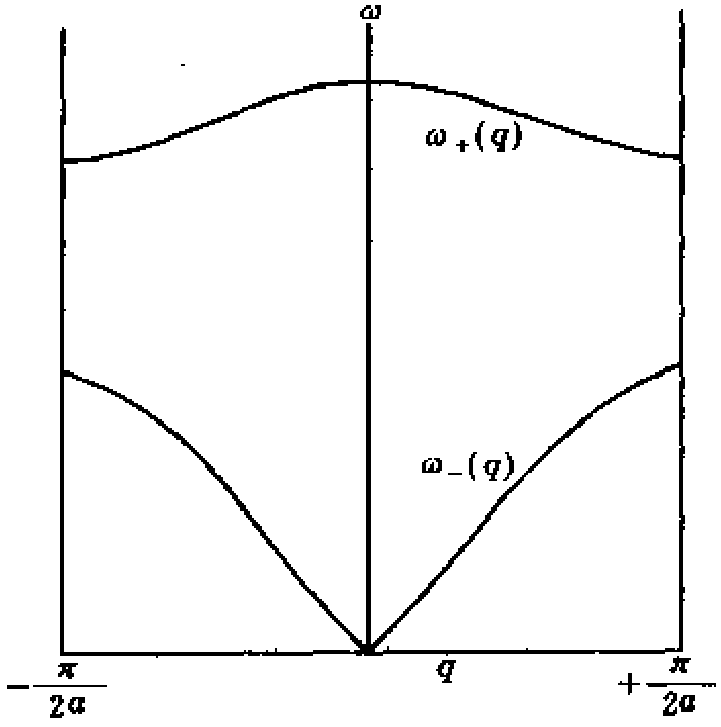
\includegraphics[height=1.in,width=1.in,viewport=0 0 700 800,clip]{Figures/Optic-Acous.png}
\label{optic_acous}
\end{minipage}
\hfill
\begin{minipage}[t]{0.67\linewidth}
%\vspace*{-0.3in}
	\begin{itemize}
		\item \textcolor{blue}{光学支}:~属于频率$\omega_+$的晶格简谐振动
		\item \textcolor{blue}{声学支}:~属于频率$\omega_-$的晶格简谐振动
	\end{itemize}
\end{minipage}
\caption{\tiny \textrm{The acoustic branch and optical branch.}}%
\end{figure} 
声学支的长波极限($q\rightarrow0$):
\begin{displaymath}
	\omega_-\approx a\sqrt{\frac{2\beta}{m+M}}q\quad\mbox{\textcolor{blue}{一维链看成连续介质的弹性波}}
\end{displaymath}
光学支的长波极限($q\rightarrow0$):
\begin{displaymath}
	\omega_+\approx a\sqrt{\frac{2\beta}{\left( \frac{mM}{m+M} \right)}}\quad\mbox{\textcolor{blue}{两种原子具有相反的相位,质心保持不动}}
\end{displaymath}
}

\frame
{
	\frametitle{声子振动模式的横向传播与纵向传播}
\begin{figure}[h!]
\centering
%\hspace*{-10pt}
\vspace*{-0.30in}
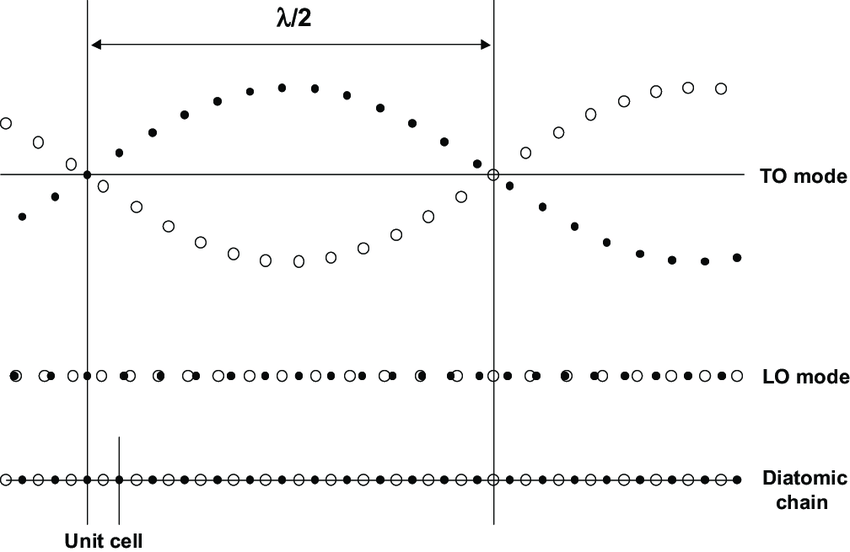
\includegraphics[height=2.5in,width=4.0in,viewport=0 0 850 610,clip]{Figures/examples-of-transverse-optical-to-and-longitudinal-optical-lo-phonons-in-1d.png}
\caption{\tiny \textrm{Schematic examples of transverse optical to and longitudinal optical phonons in 1d diatomic lattice.}}%
\label{To-Lo-1D}
\end{figure} 
}

\frame
{
	\frametitle{声学支和光学支的长波极限}
\begin{figure}[h!]
\centering
%\hspace*{-10pt}
\vspace*{-0.10in}
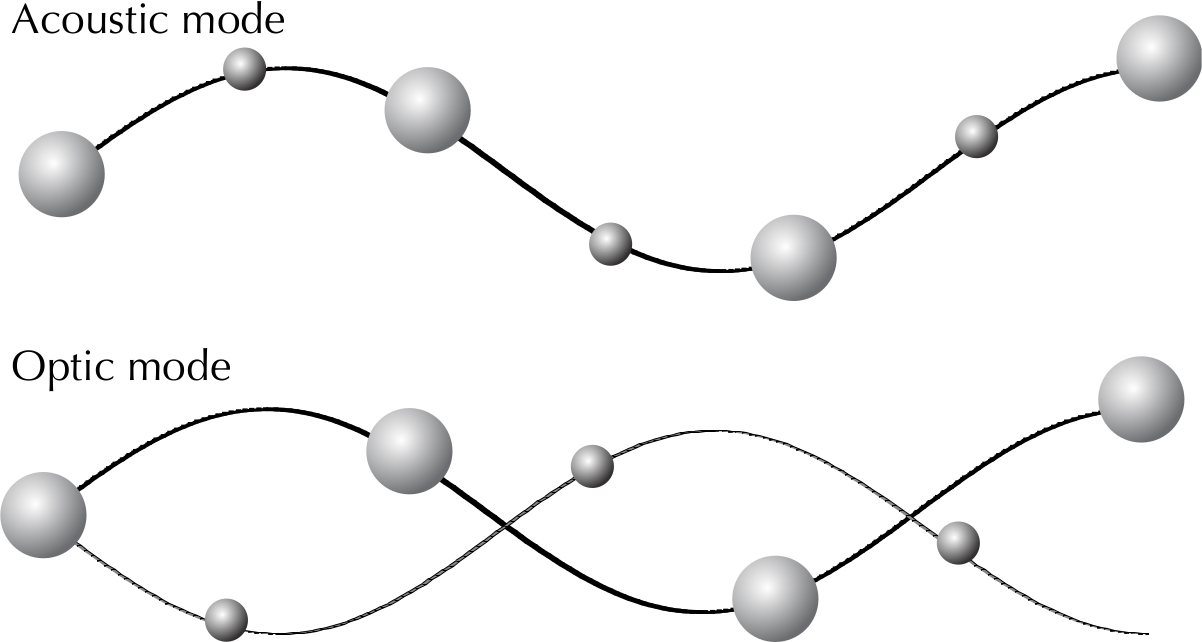
\includegraphics[height=2.3in,width=4.0in,viewport=0 0 1210 650,clip]{Figures/Phonon-Acoutic-Optic.png}
\caption{\tiny \textrm{Representation of the difference between acoustic and optic modes in the limit of wave vector $\vec q\rightarrow0$ for the model diatomic chain: acoustic (in-phase) and optic (out-of-phase) modes.}}%
\label{Aucous-Optic}
\end{figure} 
}

\frame
{
	\frametitle{经典三维振动模式}
	位于$\mathbf{R}_I(t)$的原子核运动的经典力学描述
			\begin{displaymath}
				M_I\frac{\partial^2\mathbf{R}_I}{\partial t^2}=\vec F_I(\mathbf{R})=-\frac{\partial}{\partial\mathbf{R}_I}E(\mathbf{R})
			\end{displaymath}
			晶格平衡位置$\{\mathbf{R}_I^0\}=\mathbf R^0$由原子核受力平衡确定
			\begin{displaymath}
				\vec F_I(\mathbf R^0)=0
			\end{displaymath}
			\textcolor{blue}{对平衡位置偏移的受力方程为}
			\begin{displaymath}
				C_{I,\alpha;J,\beta}=\frac{\partial^2E(\mathbf{R})}{\partial\mathbf{R}_{I,\alpha}\partial\mathbf{R}_{J,\beta}}
			\end{displaymath}
			其中$\alpha,\beta\cdots$是\textrm{cartesian}坐标

			\textcolor{blue}{谐振子近似下},频率为$\omega$的谐振模式下,晶格对平移位置的偏移为
			\begin{displaymath}
				\mathbf{u}_I(t)=\mathbf{R}_I(t)-\mathbf{R}_I^0\equiv\mathbf{u}_I\mathrm{e}^{\mathrm{i}\omega t}
			\end{displaymath}
}

\frame
{
	\frametitle{三维晶格振动模式}
			对位于$I$的原子核(质量为$M_I$),有
			\begin{displaymath}
				-\omega^2M_Iu_{I\alpha}=-\sum_{J\beta}C_{I,\alpha;J\beta}u_{J\beta}
			\end{displaymath}
			因此振动频率$\omega$,由经典谐振方程确定
%			\begin{displaymath}
%				\det\left|\frac1{\sqrt{M_IM_J}}C_{I,\alpha;J\beta}-\omega^2\right|=0
%			\end{displaymath}
%	对于周期性的晶格振动,根据\textrm{Bl\"och~}定理,振动引起的位置偏移
%			\begin{displaymath}
%				\mathbf{u}_s(\vec T_n)\equiv\mathbf{R}_s(\vec T_n)-\mathbf{R}_s^0(\vec T_n)=\mathrm{e}^{\mathrm{i}\vec k\cdot\vec T_n}\mathbf{u}_s(\vec k)
%			\end{displaymath}
%			由此得谐振方程
			\begin{displaymath}
				\det\left|\frac1{\sqrt{M_sM_{s^{\prime}}}}C_{s,\alpha;s^{\prime}\alpha^{\prime}}-\omega_{i\vec k}^2\right|=0
			\end{displaymath}
			这里原子标记$s=1,\cdots,s$,对应的谐振模式$i=1,\cdots,3s$

			每个$\vec k$的约化力常数矩阵可表示为
			\begin{displaymath}
				\begin{aligned}
				C_{s,\alpha;s^{\prime}\alpha^{\prime}}(\vec k)=&\sum_{\vec T_n}\mathrm{e}^{\mathrm{i}\vec k\cdot\vec T_n}\frac{\partial^2 E(\mathbf{R})}{\partial\mathbf{R}_{s,\alpha}(0)\partial\mathbf{R}_{s^{\prime},\alpha^{\prime}}(\vec T_n)}\\
				=&\frac{\partial^2E(\mathbf{R})}{\partial\mathbf{u}_{s,\alpha}(\vec k)\partial\mathbf{u}_{s^{\prime},\alpha^{\prime}}(\vec k)} 
				\end{aligned}
			\end{displaymath}
}

\subsection{分子动力学提要}
\frame
{
	\frametitle{分子动力学\textrm{(MD)}}
	分子动力学\textrm{(Molecular dynamics,~MD)}主要用于各类化学反应、合金与复杂材料状态方程研究,着重关注体系的反应或状态随温度、压力变化规律和动力学性质
\vskip 5pt
\textcolor{blue}{分子动力学模拟的基本框架}
	\begin{itemize}
		\item 结构优化:~根据体系的初始构型\textrm{(initial configuration)},遵从能量最低原理,得到体系基态结构(确定基态时原子的位置)
		\item 原子运动计算:~在一定环境(温度、压力等)条件下,计算各原子的受力,并依据运动方程得到设定时间步长下的原子的运动,进而获得得体系的当前构型
		\item 径迹计算:~在设定的时间范围内,根据原子运动和体系构型的变化,组合成体系随时间演化的径迹\textrm{(the trajectory of time evolution)}
		\item 结果分析:~分析体系的径迹变化规律,得到体系的动力学和热力学性质
	\end{itemize}
}

\subsubsection{经典分子动力学简介}
\frame
{
	\frametitle{经典分子动力学}
	装有$N$个经典粒子的$L_1\times L_2\times L_3$容器内,假设粒子间只有简单的二体相互作用\footnote{\fontsize{7.2pt}{6.2pt}\selectfont{二体作用是粒子间多体相互作用的简化,只考虑粒子两两间彼此相互作用。}}$\vec F(r)$,力的大小仅与粒子间间距$r$相关
	\begin{displaymath}
		\vec F(R_i)=\sum_{\substack{j=1\\j\neq i}}^N F(|\vec r_i-\vec r_j|)\hat{\vec r}_{ij}
	\end{displaymath}
	{\fontsize{7.2pt}{6.2pt}\selectfont{这里$R$代表全部原子坐标$\vec r_i$,$\hat{\vec r}_{ij}$是表示粒子$i$指向粒子$j$的矢量($\vec r_j-\vec r_i$)的单位矢量}}

	在经典力学框架下,粒子$i$的受力运动方程是:~
	\begin{displaymath}
		\dfrac{\mathrm{d}^2\vec r_i(t)}{\mathrm{d}t^2}=\dfrac{\vec F_i(R)}{m_i}
	\end{displaymath}
	粒子$i$的质量是$m_i$\\
	\textcolor{purple}{经典分子动力学,就是应用数值模拟对大量粒子求解该方程,基于统计力学原理,研究物质的状态和热力学性质}
}

\frame[allowframebreaks]
{
	\frametitle{经典分子动力学力场}
	原子间受力一般用\textcolor{red}{力场}(\textrm{Force Field},也就是“\textcolor{blue}{相互作用势}”)描述,力场的形式有很多种,典型力场的有
	\begin{itemize}
		\item \textrm{Lennard-Jones}对势
	\begin{displaymath}
		U(r)=4\varepsilon\bigg[\bigg(\dfrac{\sigma}{r}\bigg)^{12}-\bigg(\dfrac{\sigma}{r}\bigg)^6\bigg]
	\end{displaymath}
	{\fontsize{7.2pt}{6.2pt}\selectfont{这里$\varepsilon$和$\sigma$是和原子有关的参数
	\textrm{L-J}势能的最低点在$r_{\min}=2^{(1/6)}\sigma\approx1.12\sigma$,$r<r_{\min}$时为排斥力,$r>r_{\min}$时为吸引力
\begin{figure}[h!]
\centering
\vspace*{-0.30in}
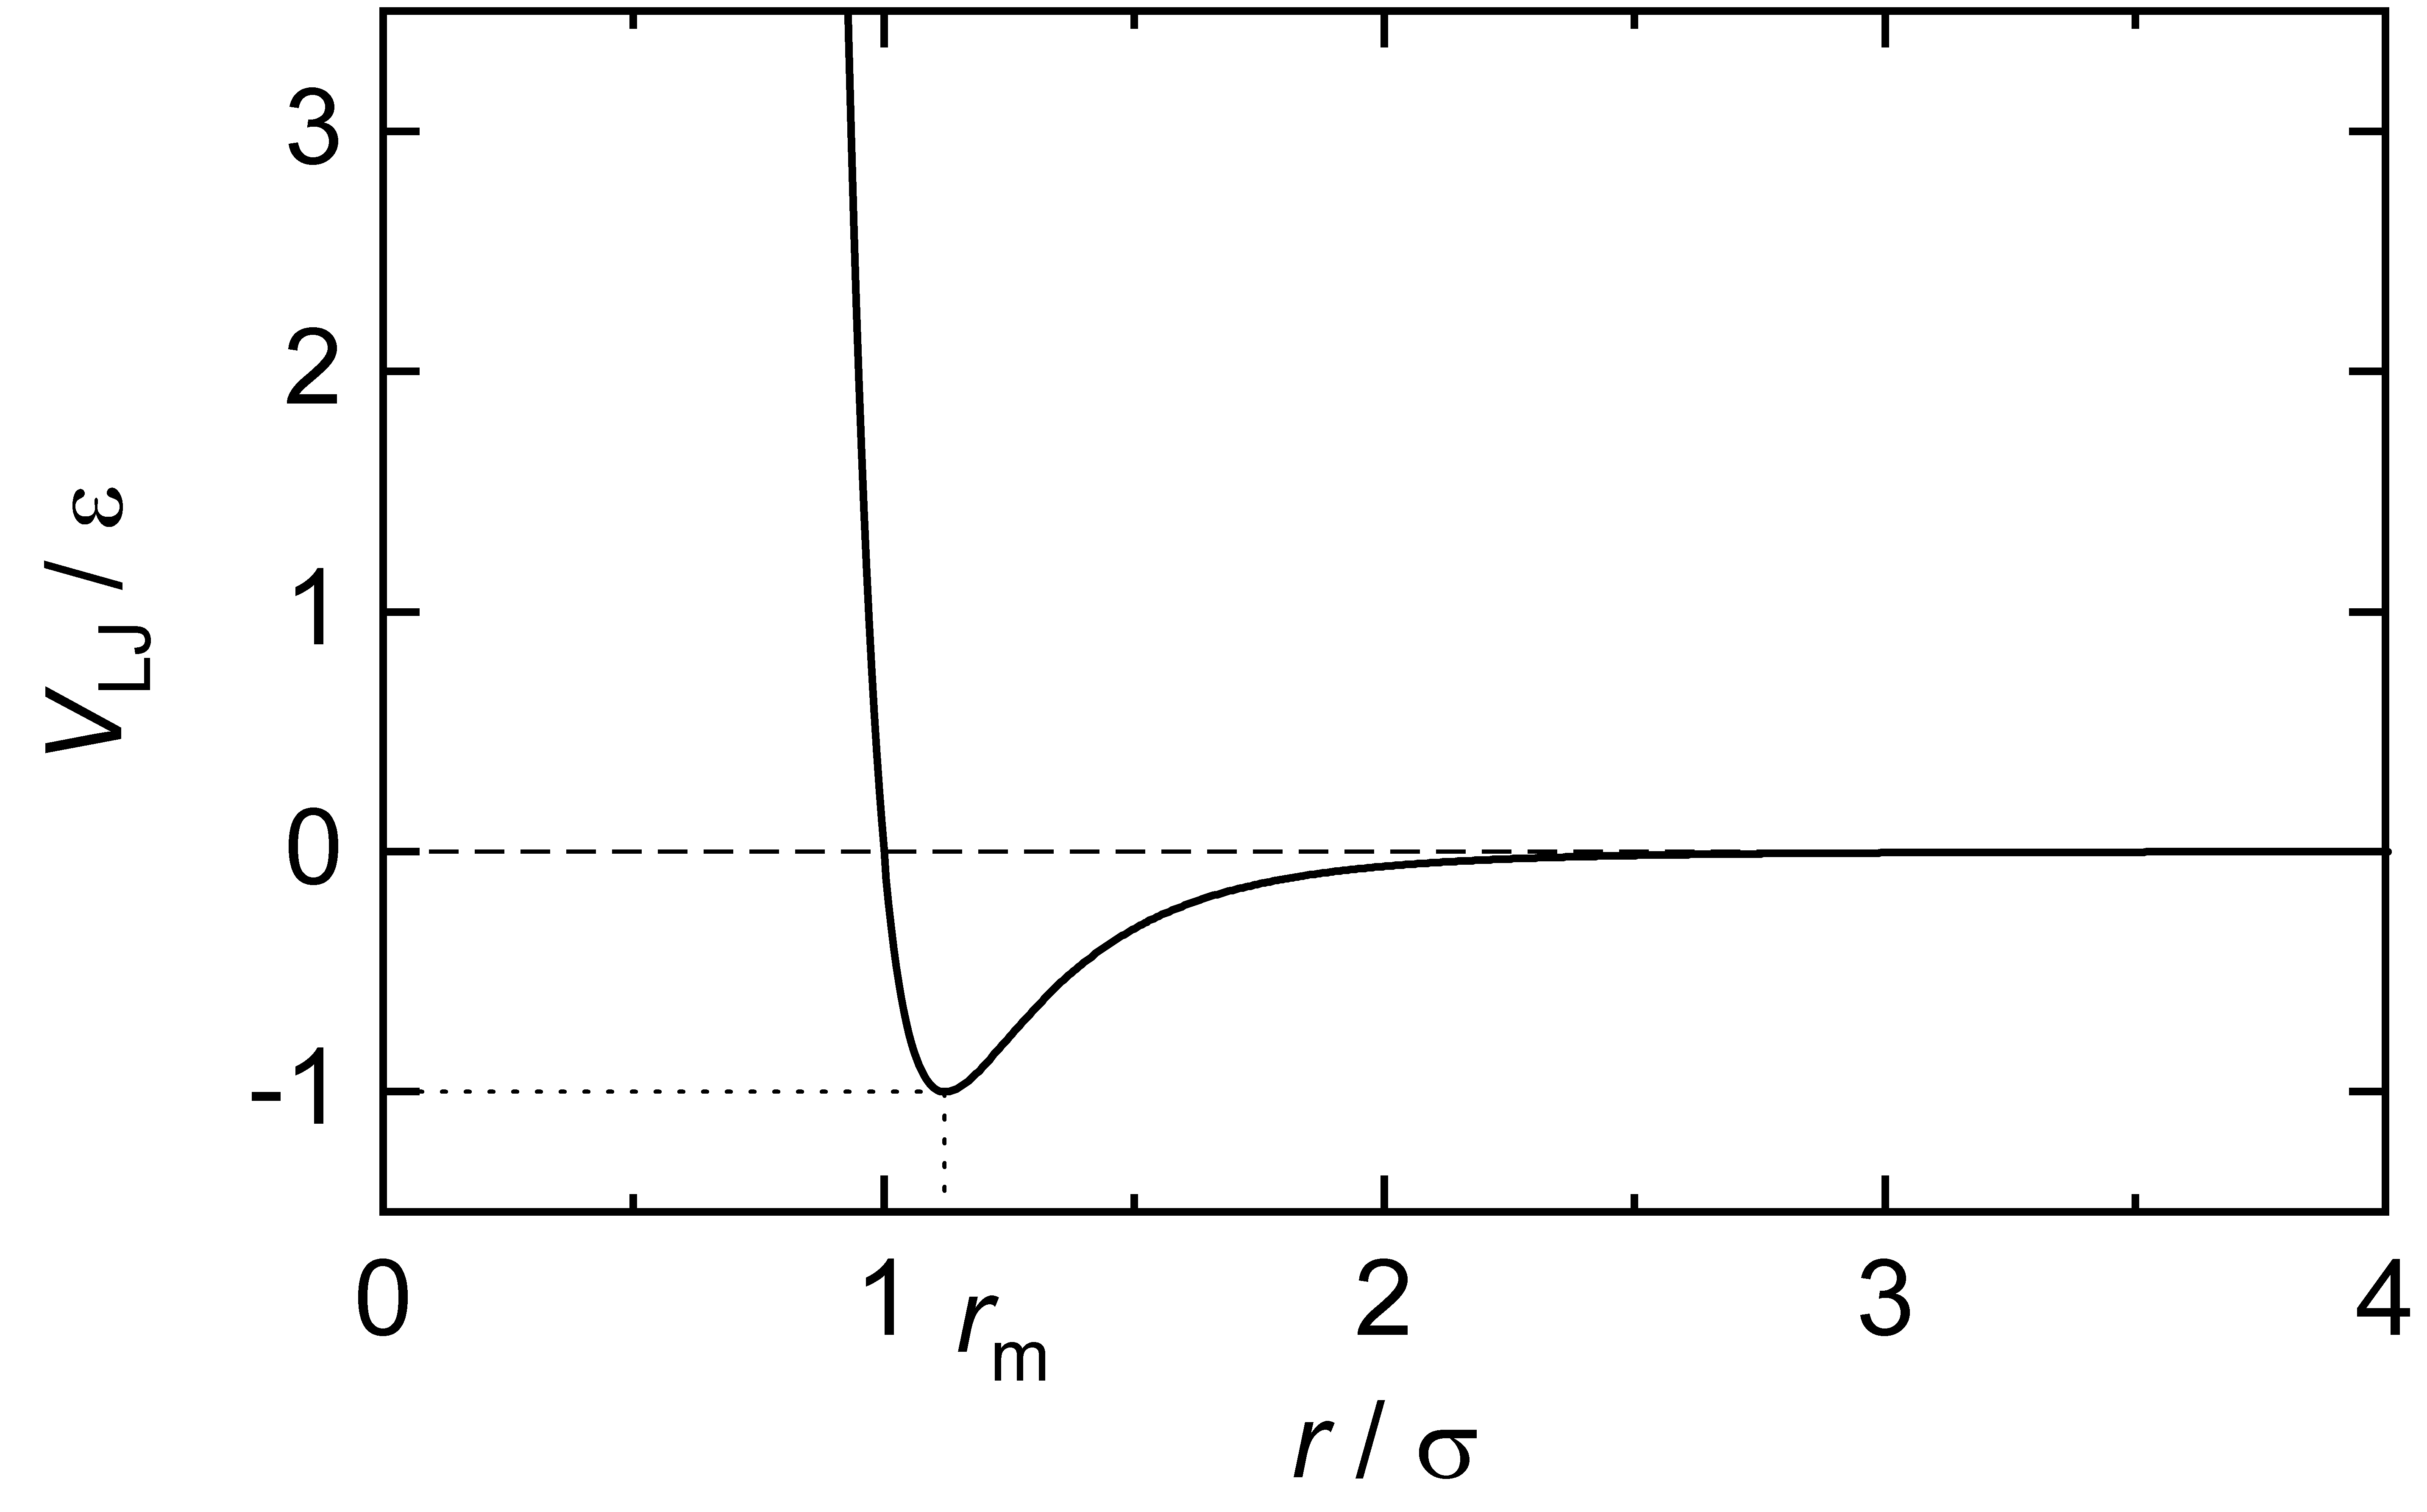
\includegraphics[height=1.00in,width=1.35in,viewport=0 0 340 270,clip]{Figures/Lennard-Jones_potential.png}
\caption{\tiny \textrm{The Lennard-Jones Potential.}}%(与文献\cite{EPJB33-47_2003}图1对比)
\label{Potential-Lennard-Jones}
\end{figure}
\vskip -20pt
	由\textrm{L-J}势改造,可以得到\textrm{WCA}势和\textrm{PHS}势}}
\item \textrm{Morse}势
	\begin{displaymath}
		U(r)=-D_{\mathrm{e}}+D_{\mathrm{e}}\bigg(1-\mathrm{e}^{-a(r-r_{\mathrm{e}})}\bigg)^2
	\end{displaymath}
	{\fontsize{7.2pt}{6.2pt}\selectfont{这里$D_{\mathrm{e}}$是\textrm{Morse}势的势阱深,参数$a$确定势阱宽度,$r_{\mathrm{e}}$是原子处于平衡位置的平衡键长
\begin{figure}[h!]
\centering
\vspace*{-0.15in}
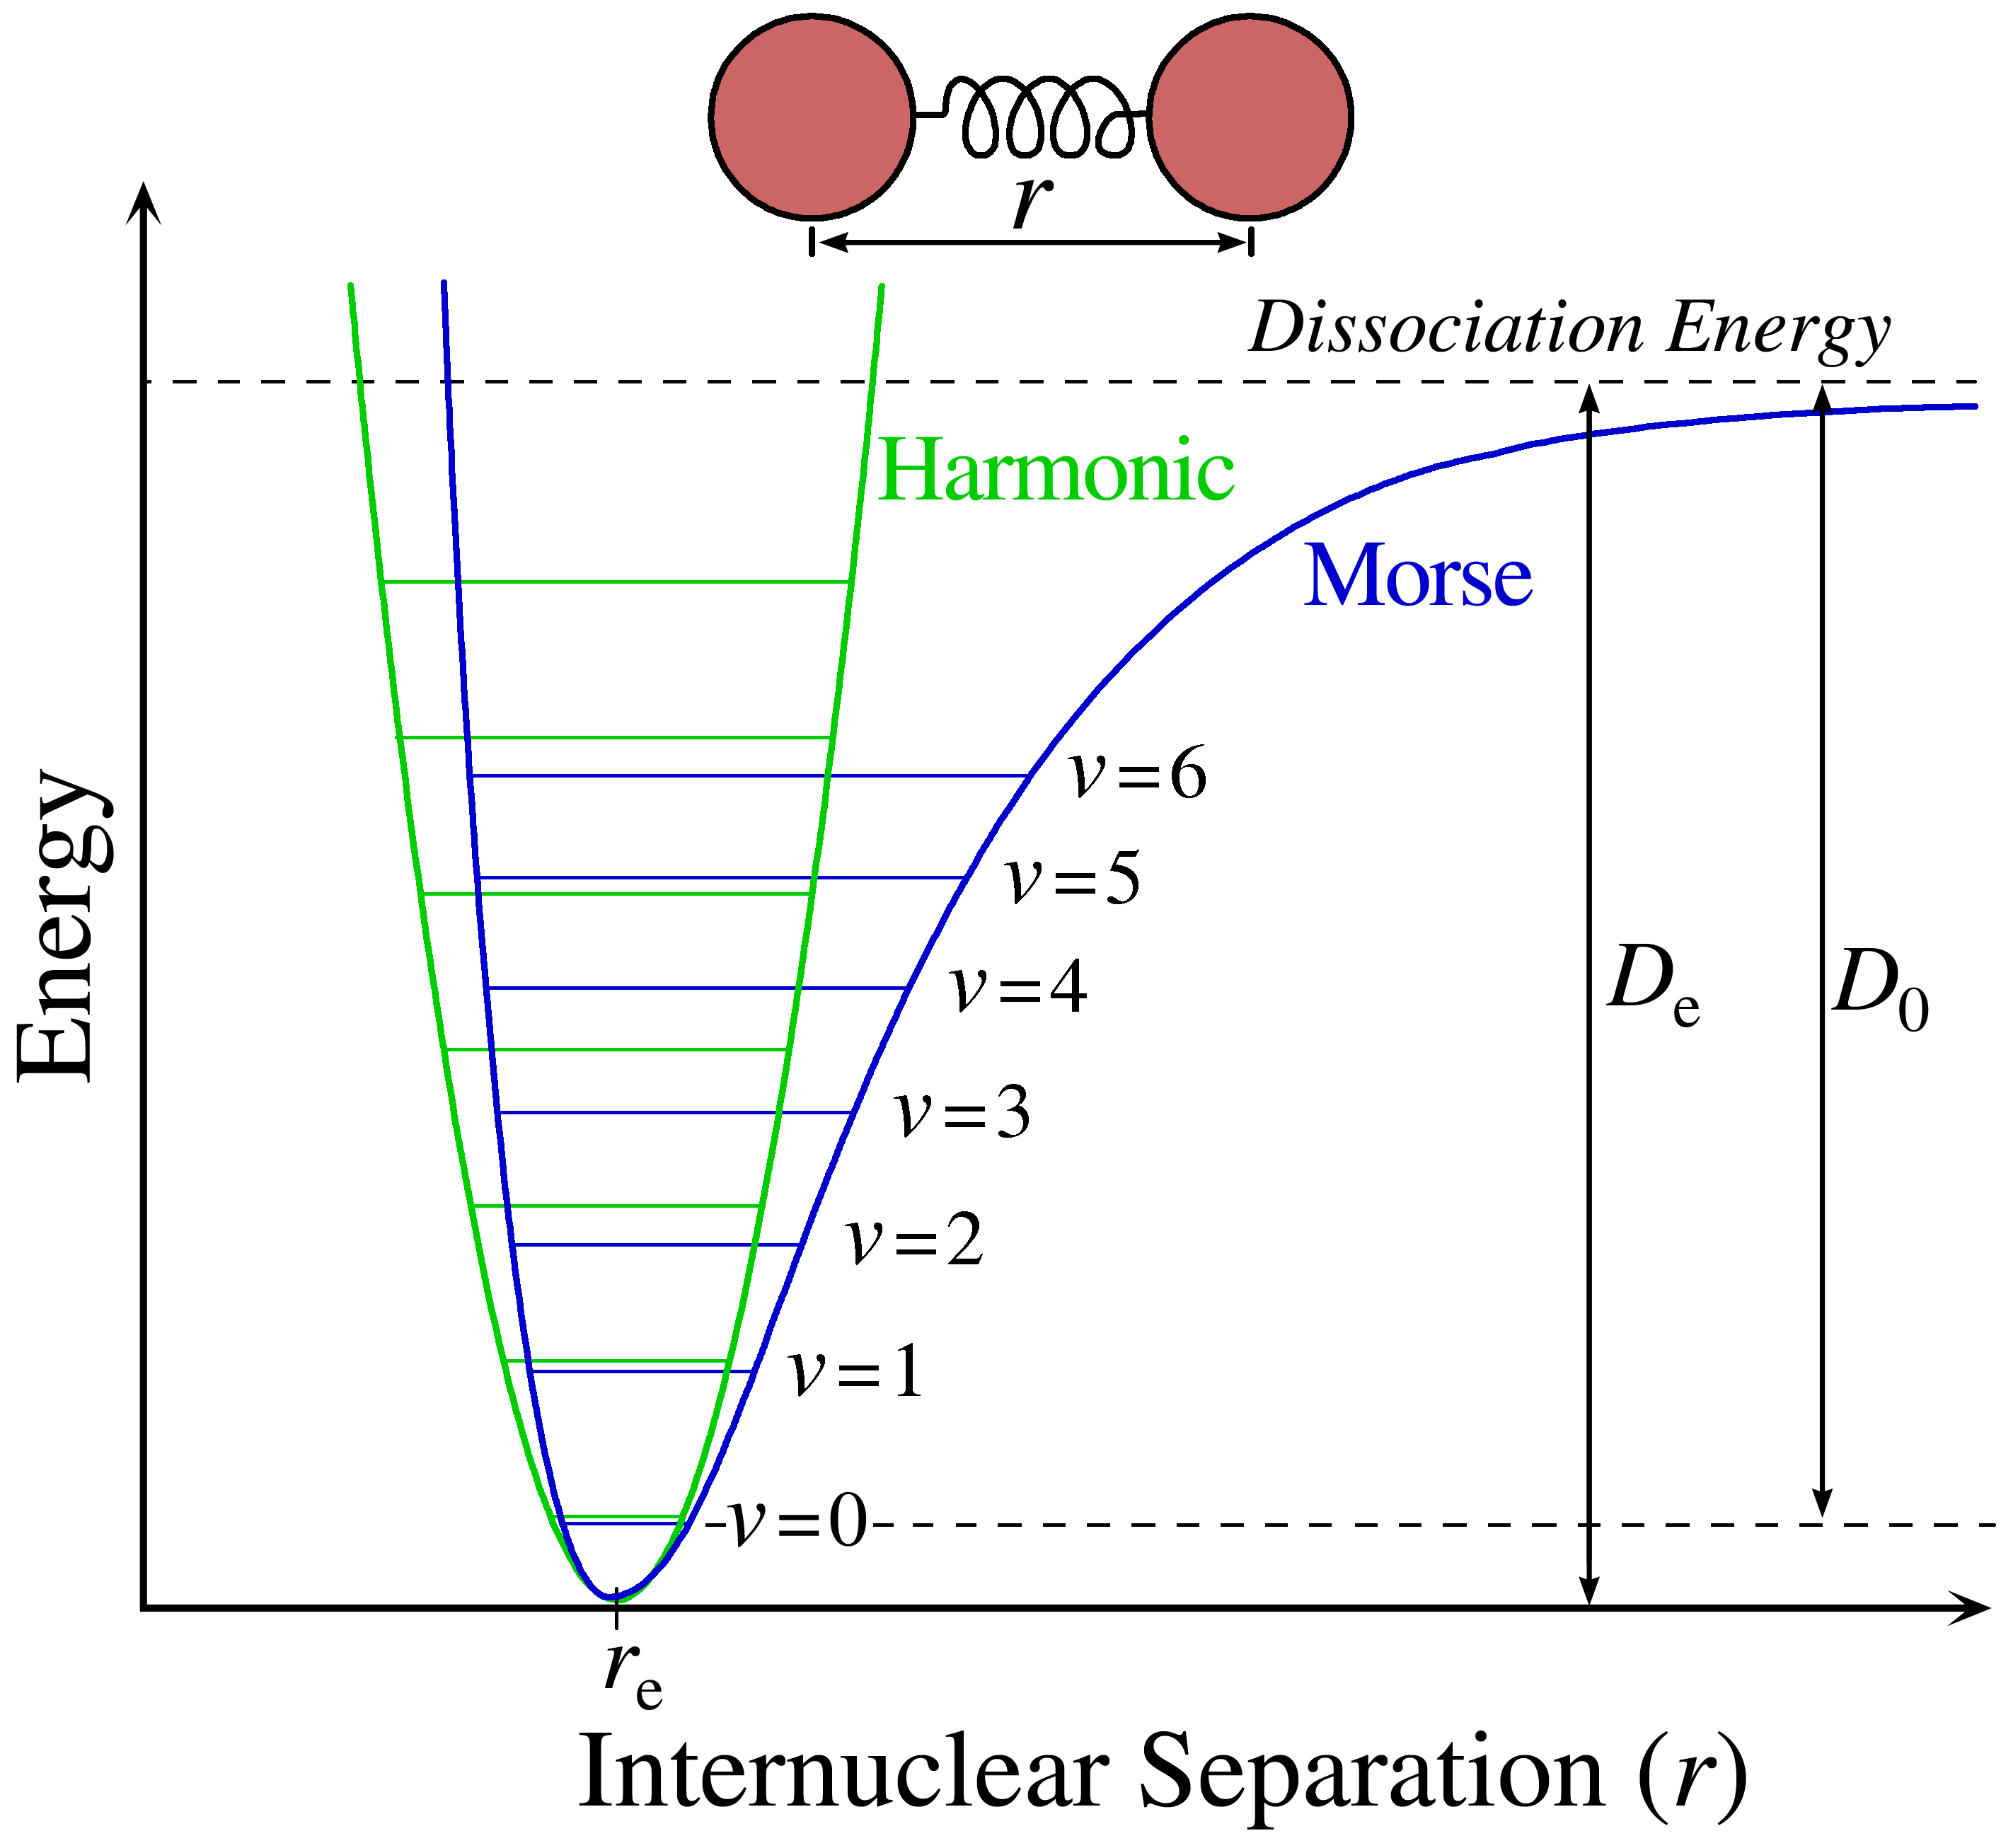
\includegraphics[height=1.30in,width=1.85in,viewport=0 0 3540 2770,clip]{Figures/Morse-potential.png}
\caption{\tiny \textrm{The Morse potential (blue) and harmonic oscillator potential (green).}}%(与文献\cite{EPJB33-47_2003}图1对比)
\label{Potential-Morse}
\end{figure}
}}
\item \textrm{EAM}势\\
	{\fontsize{7.2pt}{6.2pt}\selectfont{对于金属晶体,内能虽可以表示为对相互作用之和,但拟合原子受力非常困难:\footnote{\fontsize{5.2pt}{3.2pt}\selectfont{应用二体势计算金属弹性常数时必须涉及对体积很敏感的能量项,因为涉及缺陷、表面的体积很难确定。}}\\
	\textcolor{red}{从物理上说金属原子处于电子海洋中,电子密度来自多个原子的贡献,这是自由电子气带来的多体效应}}}\\
	\textrm{EAM}将金属中原子的势能表示为二体势和多体势之和
	\begin{displaymath}
		E_i=F_{\alpha}\bigg(\sum_{j\neq i}\rho_{\beta}(r_{ij})\bigg)+\dfrac12\sum_{j\neq i}\phi_{\alpha\beta}(\vec r_{ij})
	\end{displaymath}
	{\fontsize{7.2pt}{6.2pt}\selectfont{$\alpha$和$\beta$分别为位置$i$、$j$处的原子类型\\
		$\phi$是二体势,是原子$\alpha$和$\beta$和原子间距$r_{ij}$的函数\\
		$F$是多体势,是其余原子在位置$i$处的电荷密度与位置$i$处原子$\alpha$的相互作用能,由原子类型$\alpha$和位置$i$处的电子密度确定\\
		位置$j$原子在位置$i$处产生的电荷密度$\rho$只与位置$j$处原子类型$\beta$和原子间距$r_{ij}$有关,与方向无关
	}}\\
	各类\textrm{EAM}势中,$\phi(r)$、$\rho(r)$和$F(\rho)$都不是解析的,以数值形式存储
	\end{itemize}
}

\frame
{
	\frametitle{经典分子动力学与\textrm{Verlet}算法}
	分子动力学模拟研究的对象是平衡态体系
	\begin{itemize}
		\item 初始化
		\item 开始分子运动模拟,直到模拟体系达到平衡
		\item 继续模拟体系的物理性质,保存计算结果
	\end{itemize}
	\textcolor{blue}{标准\textrm{Verlet}算法:~}求解作用力$\vec F$下单个粒子运动的积分
	\begin{displaymath}
		\vec r(t+h)=2\vec r(t)-\vec r(t-h)+h^2\vec F(\vec r(t))/m
	\end{displaymath}
	{\fontsize{7.2pt}{6.2pt}\selectfont{这里$h$是时间步长,$t=nh$是模拟累积时间,$\vec r(t)$是粒子在时间$t$时的位置\\
	\textcolor{magenta}{每个时间步长的误差为$h^4$,在模拟时间范围内的累积误差是$h^2$}
\vskip 5pt
	{\fontsize{7.2pt}{6.2pt}\selectfont{如果已知模拟粒子的初始速度$\vec v$和时间,取初始态时间$t=0$}}
	\begin{displaymath}
		\vec r(h)=\vec r(0)=h\vec v(0)+\dfrac{h^2}2\vec F[\vec r(t=0)]~\qquad~ (m\equiv1)
	\end{displaymath}
误差为$h^3$,速度随时间变化的函数
\begin{displaymath}
	\vec v(t)=\dfrac{\vec r(t+h)-\vec r(t-h)}{2h}+\mathscr{O}(h^2)
\end{displaymath}
}}
}

\frame
{
	\frametitle{经典分子动力学与\textrm{Verlet}算法}
	\textrm{Verlet}算法有两种被普遍应用的变体形式,相比于标准\textrm{Verlet}算法,这两种方法误差累积效应更小
	\begin{itemize}
		\item \textcolor{blue}{蛙跳(\textrm{Leap-Frog})法}
			\begin{displaymath}
				\begin{aligned}
					\vec v(t+h/2)=&\vec v(t-h/2)+h\vec F[\vec r(t)]\\
					\vec r(t+h)=&\vec r(t)+h\vec v(t+h/2)
				\end{aligned}
			\end{displaymath}
		\item \textcolor{blue}{速度-\textrm{Verlet}算法}
			\begin{displaymath}
				\vec v(t)=\dfrac{\vec r(t+h)-\vec r(t-h)}{2h}
			\end{displaymath}
			\begin{displaymath}
				\begin{aligned}
					\vec r(t+h)=&\vec r(t)+h\vec v(t)+h^2\vec F(t)/2\\
					\vec v(r+h)=&\vec v(t)+h[\vec F(t+h)+\vec F(t)]/2
				\end{aligned}
			\end{displaymath}
			速度-\textrm{Verlet}算法更稳定也更方便,但需要保存$\vec F(t)$和$\vec F(t+h)$两个力的数组
	\end{itemize}
}

\frame
{
	\frametitle{经典分子动力学与\textrm{Verlet}算法}
	以下算法与速度-\textrm{Verlet}算法完全等价,但只需要保留$\vec F(t)$一个数组
	\begin{displaymath}
		\begin{aligned}
			\tilde{\vec v}(t)=&\vec v(t)+h\vec F(t)/2\\
			\vec r(t+h)=&\vec r(t)+h\tilde{\vec v}(t)\\
			\vec v(t+h)=&\tilde{\vec v}(t)+h\vec F(t+h)/2
		\end{aligned}
	\end{displaymath}
	而粒子受力$\vec F(t+h)$则在第二步、第三步之间临时计算
\vskip 5pt
	{\fontsize{6.2pt}{4.2pt}\selectfont{一般地,作用在粒子$i$上的力,是所有与粒子$i$的相互作用的“合成”结果
	\begin{displaymath}
		\vec F_i(R)=-\dfrac{\partial U(\{\vec r_i\})}{\partial \vec r_i}
	\end{displaymath}
	通常总的势能$U(\{\vec r_i\})$拆解为各部分贡献
	\begin{displaymath}
		U(\{\vec r_i\})=\sum_iU_1(\vec r_i)+\sum_i\sum_{j>i}U_2(\vec r_i,\vec r_j)+\sum_i\sum_{j>i}\sum_{k>j}U_3(\vec r_i,\vec r_j,\vec r_k)+\cdots
	\end{displaymath}
	这里$U_1(\vec r_i)$是单体势,一般是单个粒子在外场(如重力场、电场)中的势能,与材料性质无关\\
$U_2(\vec r_i,\vec r_j)$是双体势,$U_3(\vec r_i,\vec r_j,\vec r_k)$是描述粒子间对相互作用的主要函数}}

	在分子动力学计算中,力的计算需要更多的时间,因为其计算耗时步数是$\mathscr{O}(N^2)$,\textcolor{blue}{对于周期体系,这种力的计算尤其需要谨慎}
}

\subsubsection{第一原理分子动力学简介}
\frame
{
	\frametitle{第一原理分子动力学\textrm{AIMD}中的近似}
	由于分子动力学模拟的复杂性,必须做出适当的近似。具体到第一原理分子动力学,一般有两类重要的近似:
	\begin{itemize}
		\item \textcolor{blue}{绝热近似\textrm{(adiabatic approximation)}}\\
			{\fontsize{6.2pt}{4.2pt}\selectfont{假设电子-原子核在能量层面上完全分离,彼此间没有能量传递}}
		\item \textcolor{blue}{\textrm{Born-Oppenheimer}近似}\\
			{\fontsize{6.2pt}{4.2pt}\selectfont{假设电子和原子核的运动完全解耦,对应每个时间步长的原子构型,电子可以实时处于基态\footnote{\fontsize{5.2pt}{4.2pt}\selectfont{\textrm{B-O}近似也是一种绝热近似,\textcolor{red}{但\textrm{B-O}近似下的绝热强调电子对核运动的瞬时响应}。讨论电子计算时,\textrm{B-O}近似下假设原子核是固定不动的;~在分子动力学讨论中,绝热近似强调的是电子-核运动在能量上的完整分离,而\textrm{B-O}近似则明确要求电子-核运动彼此完全解耦,且电子实时处于基态}}}}
	\end{itemize}
\begin{figure}[h!]
\centering
\vspace*{-0.25in}
%\hspace*{-10pt}
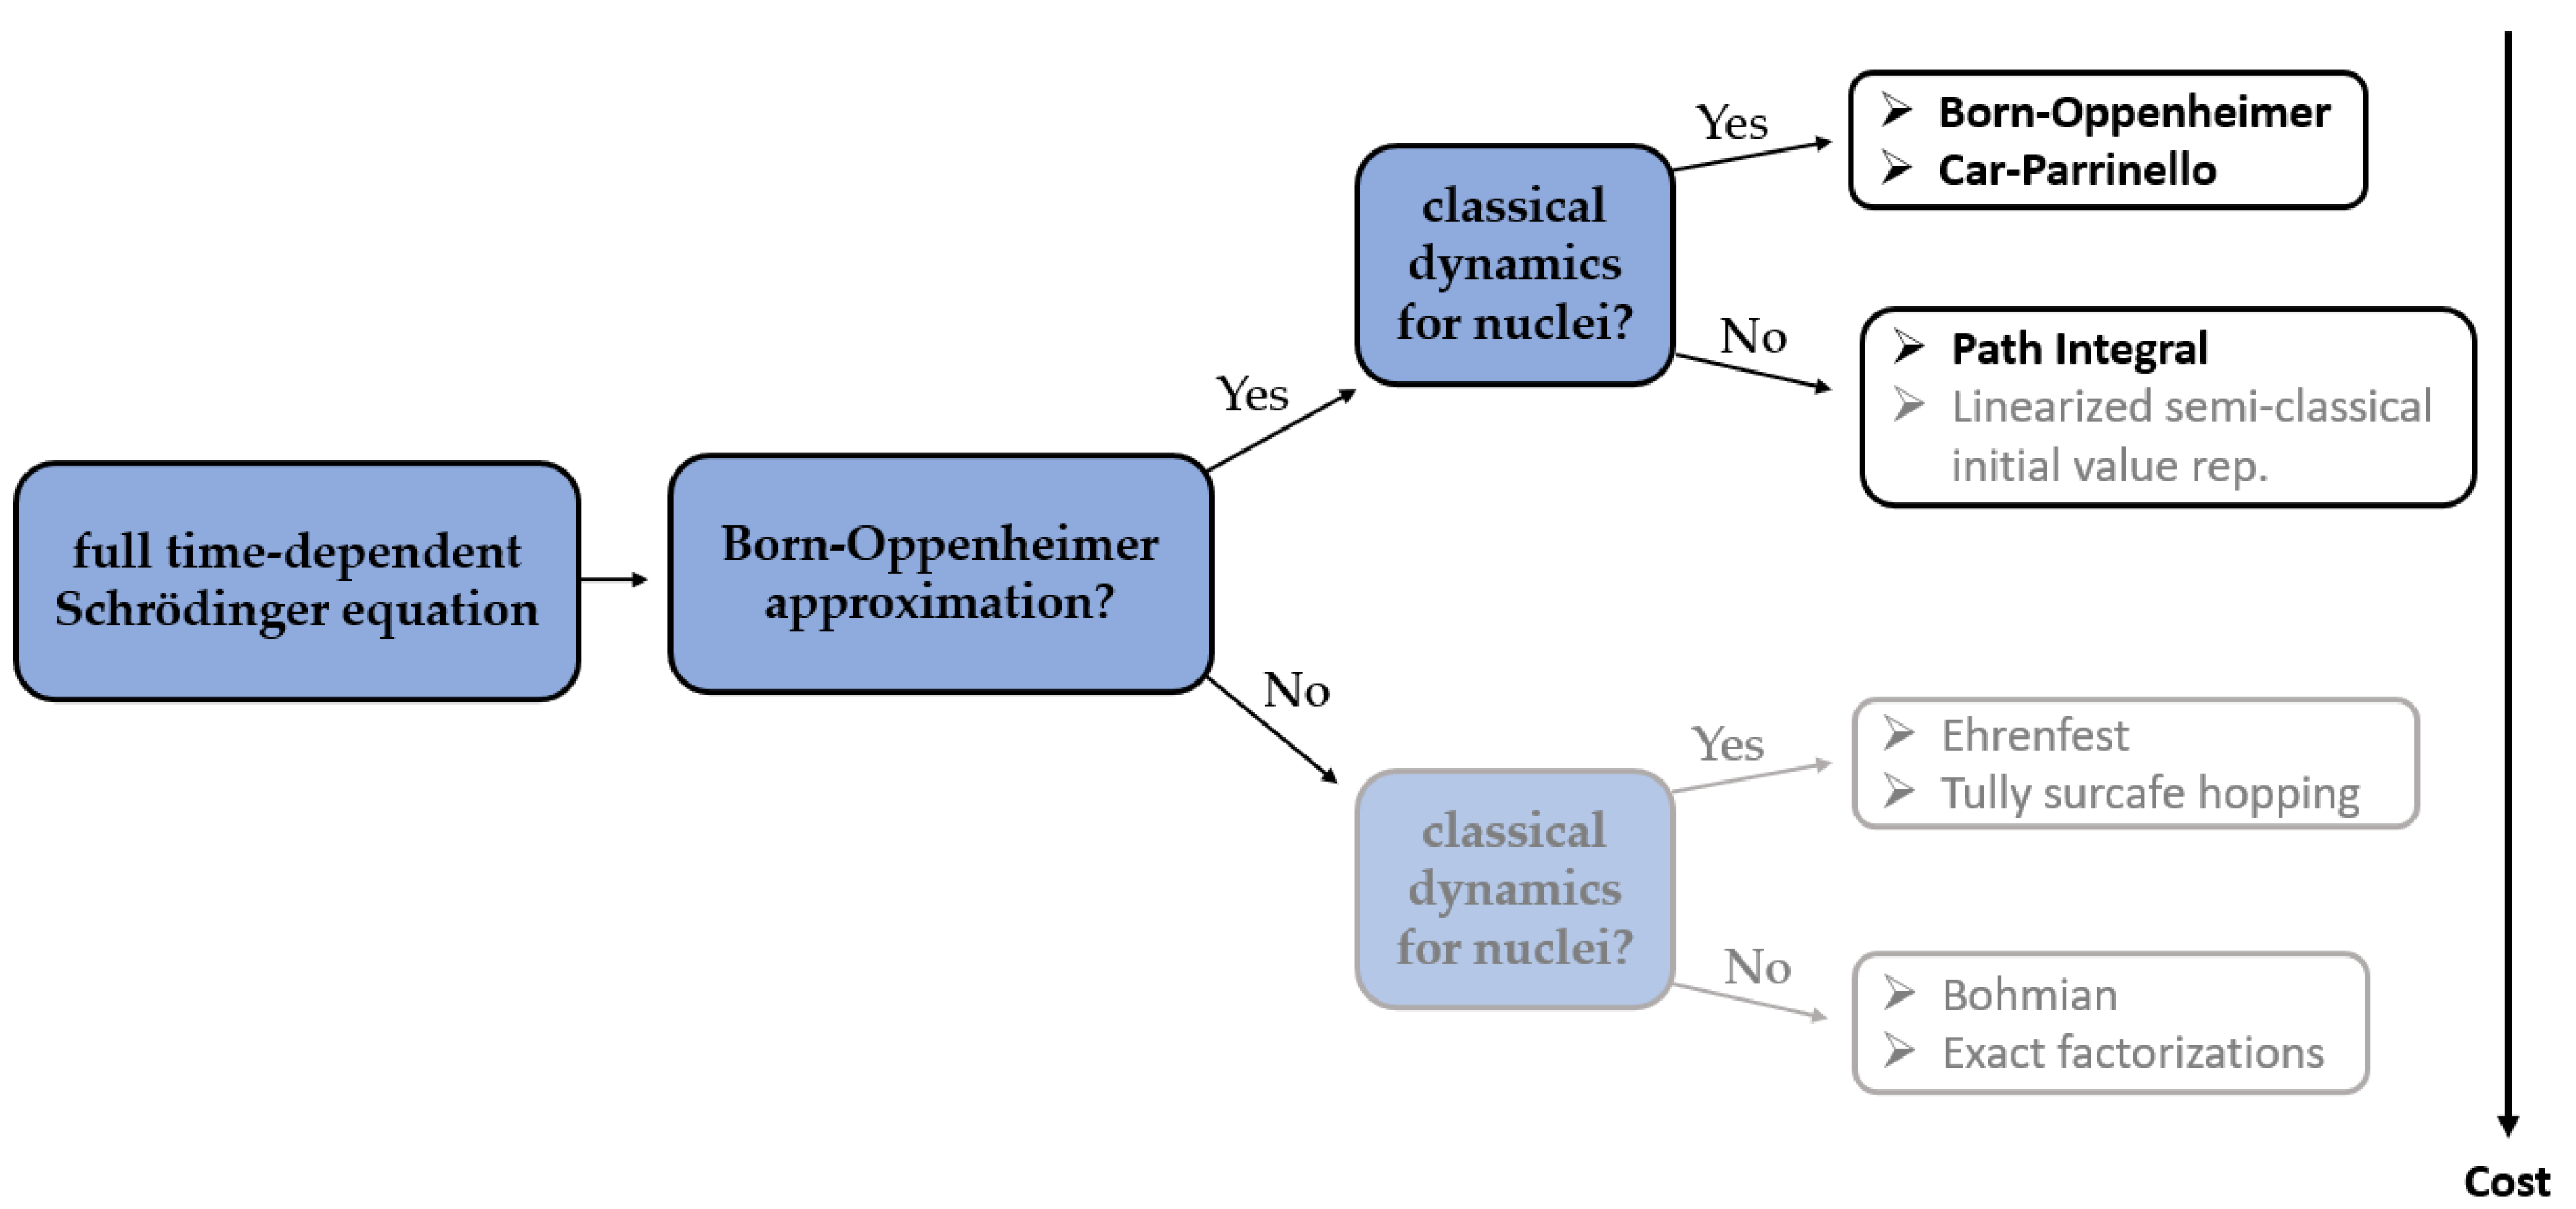
\includegraphics[height=1.55in,width=2.6in,viewport=0 0 440 230,clip]{Figures/Molecular-dynamics_Claaified.png}
%\caption{\fontsize{5.2pt}{4.2pt}\selectfont{\textrm{The major differences between the methods of aiMD simulations.}}}%
\label{Molecular-dynamics_Classified}
\end{figure}
}

\frame
{
	\frametitle{第一原理分子动力学}
	\begin{itemize}
		\item \textrm{AIMD}将电子结构与原子和经典轨迹计算在同一基础上完成
		\item 每个原子运动步的受力都是在电子结构计算基础上获得的
		\item 基于\textrm{B-O}方法:\\\textcolor{purple}{在计算原子运动径迹的每一步,都要求电子态都收敛到基态}
		\item 扩展的\textrm{Lagrangian}方法:~\textcolor{purple}{根据体系几何结构构造体系波函数}\\
			\textcolor{blue}{\textrm{Car-Parinello}}:\\
			平面波基,构成分子轨道\\
			\textcolor{blue}{\textrm{Atom-centered Density Matrix Progation~(ADMP)}}:\\
			原子中心基,构成密度矩阵
	\end{itemize}
	\textrm{AIMD}计算内容
	\begin{itemize}
		\item 可用于复杂体系的电子结构计算
		\item 几何结构优化(能量最小化)
		\item 描述系统演化
		\item 模拟时长规模$\approx{\mathrm{ps}}(10^{-12}\mathrm{s})$~(经典分子动力学 $\approx\mathrm{ns}(10^{-9}\mathrm{s})$)
	\end{itemize}
}


%\frame
%{
%	\frametitle{第一原理分子动力学的分类}
%\begin{figure}[h!]
%\centering
%\vspace*{-0.05in}
%%\hspace*{-10pt}
%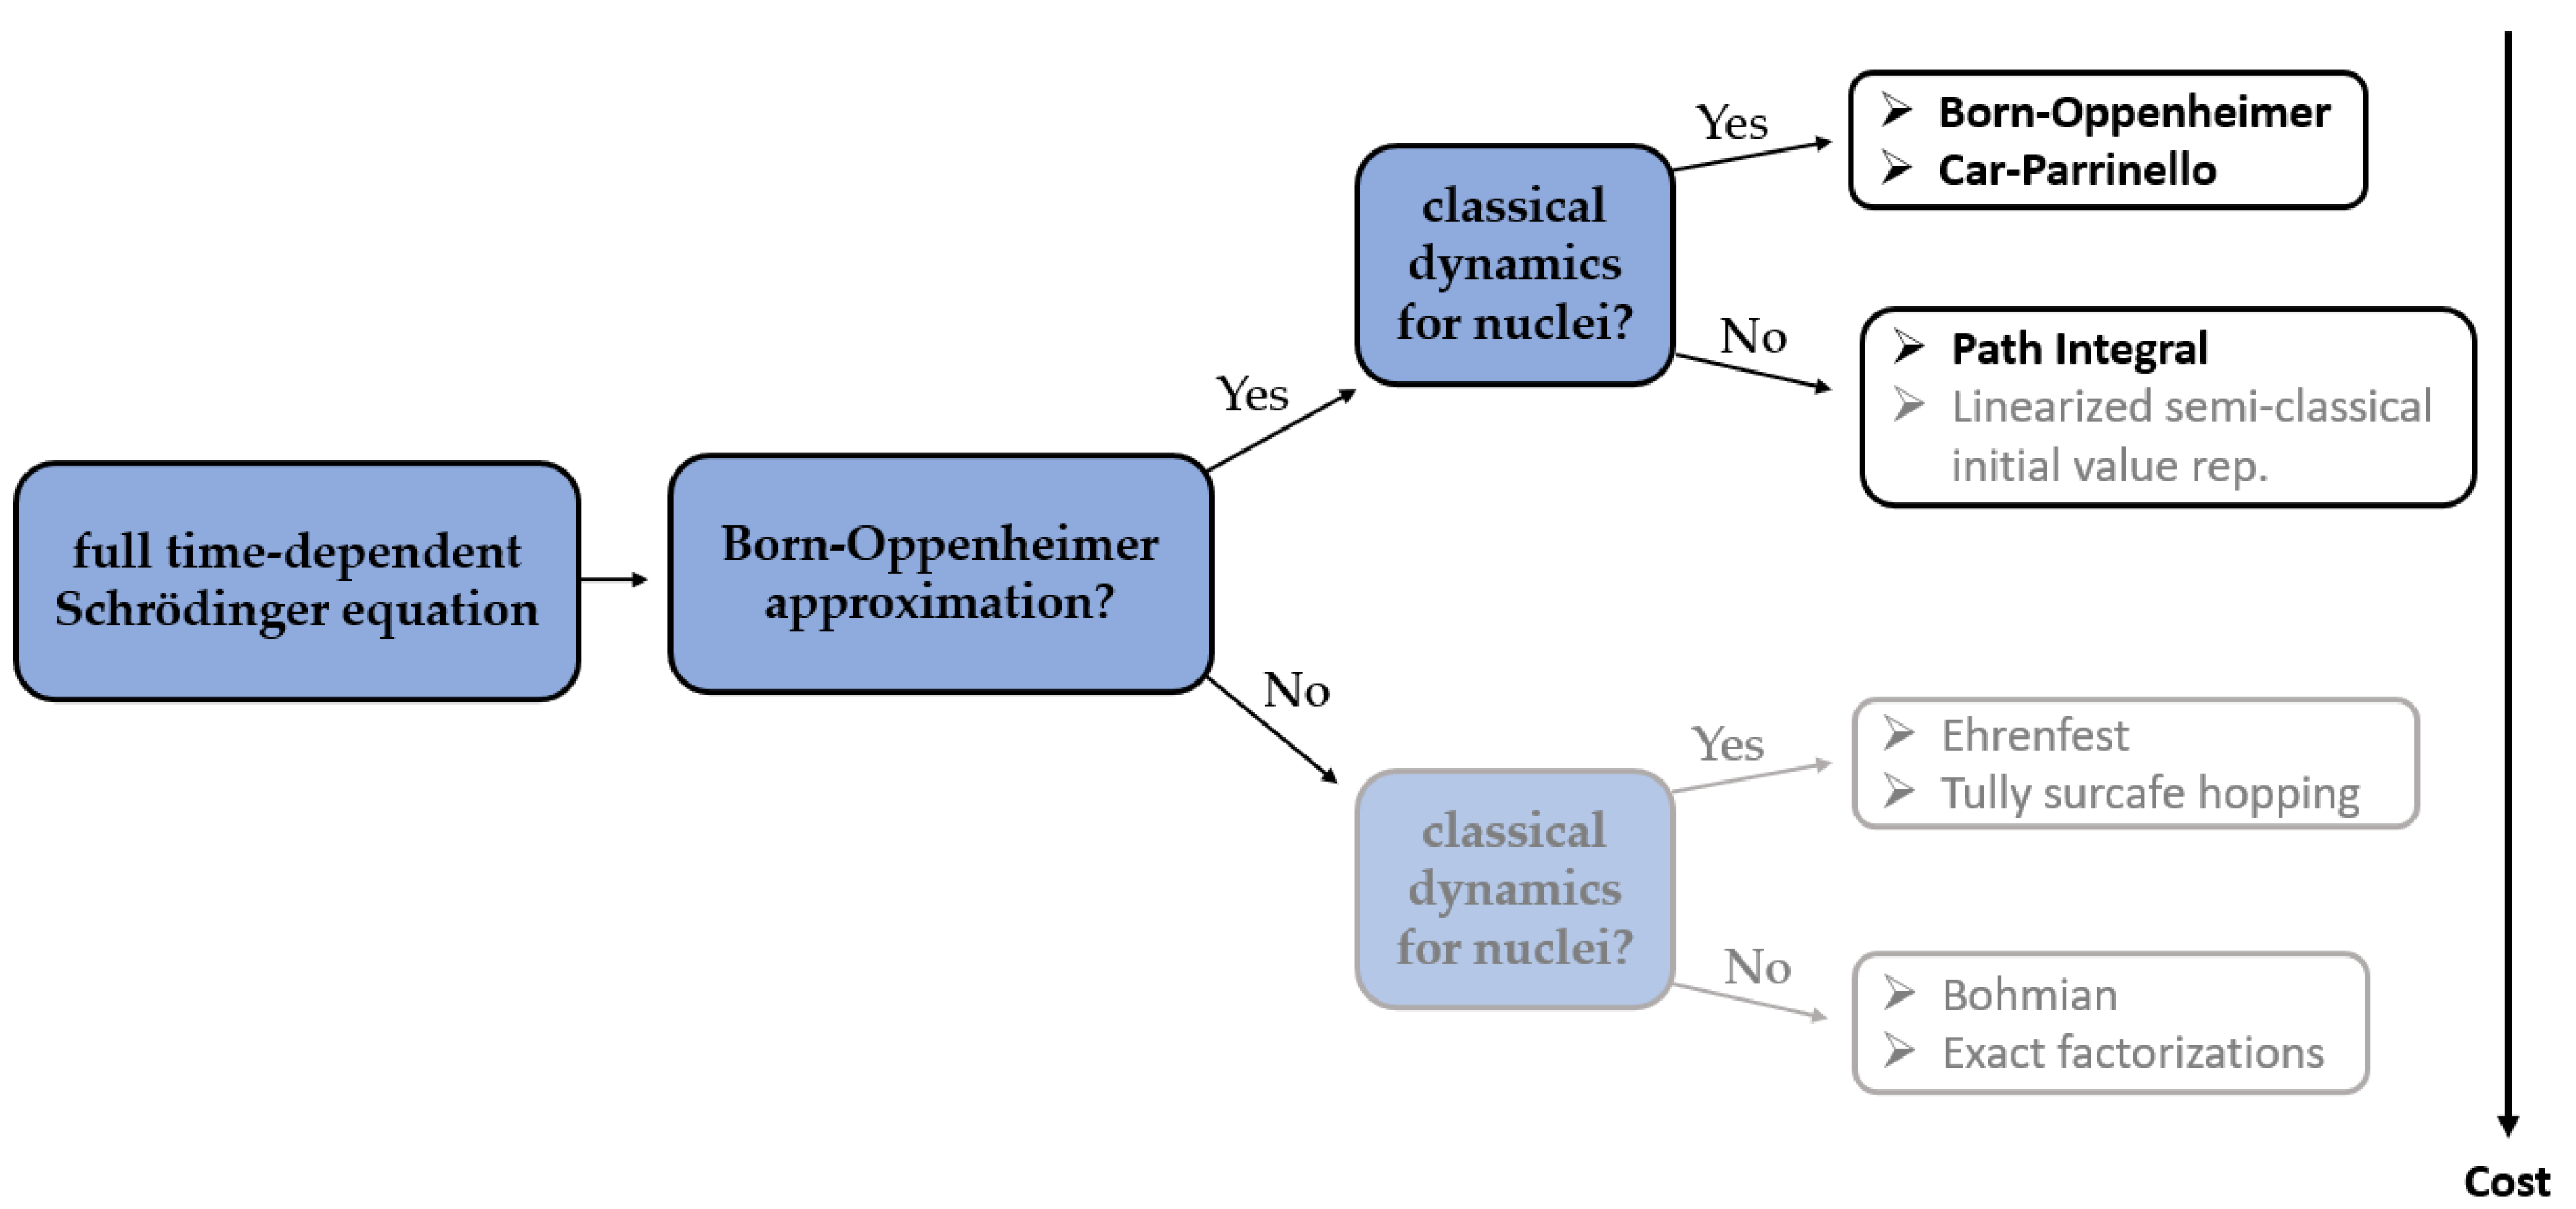
\includegraphics[height=2.3in,width=4.0in,viewport=0 0 440 230,clip]{Figures/Molecular-dynamics_Claaified.png}
%\caption{\fontsize{5.2pt}{4.2pt}\selectfont{\textrm{The major differences between the methods of aiMD simulations.}}}%
%\label{Molecular-dynamics_Claaified}
%\end{figure}
%}
%
\subsubsection{绝热近似:~\rm{Hellmann-Feynman}定理与电-声耦合}
%\frame
%{
%	\frametitle{第一原理分子动力学}
%	电子结构计算时,体系总能是基于\textrm{Born-Oppenheimer}近似得到,如果变化原子位置,可以得到体系总能随原子位置变化的规律\\
%	作为原子位置$\vec R_i$函数的电子态总能量$E(\vec R_1,\vec R_2,\cdots,\vec R_N)$称\textcolor{red}{势能面}~(\textrm{potential surface})
%
%	对于一套给定原子核位置$\mathbf{S}=(\vec R_1,\cdots,\vec R_N)$,$\vec R_i$表示第$i$个原子核的位置;~如果电子的基态波函数是$\psi_{\mathrm{G}}$则\\电子态能量为
%	\begin{displaymath}
%		E=\dfrac{\langle\psi_{\mathrm{G}}|\mathbf{H}(\mathbf{S})|\psi_{\mathrm{G}}\rangle}{\langle\psi_{\mathrm{G}}|\psi_{\mathrm{G}}\rangle}
%	\end{displaymath}
%作用在原子核$n$上的经典作用力,可由电子态能量对原子位置$\vec R_n$的梯度$\nabla_n$的负值给出
%\begin{displaymath}
%	\vec F_n=-\nabla_nE(\mathbf{S})=-\nabla_n\bigg[\dfrac{\langle\psi_{\mathrm{G}}|\mathbf{H}(\mathbf{S})|\psi_{\mathrm{G}}\rangle}{\langle\psi_{\mathrm{G}}|\psi_{\mathrm{G}}\rangle}\bigg]
%\end{displaymath}
%}
%
%\frame
%{
%	\frametitle{\textrm{Hellmann-Feynman}定理}
%	如果$\psi_{\mathrm{G}}$是\textrm{Hamiltonian}的本征态,有
%	\begin{displaymath}
%		\begin{aligned}
%			&(\langle\psi_{\mathrm{G}}|\psi_{\mathrm{G}}\rangle)^2\nabla_nE\\
%			=&\big[\langle(\nabla_n\psi_{\mathrm{G}}|\mathbf{H}|\psi_{\mathrm{G}}\rangle+\langle\psi_{\mathrm{G}}|(\nabla_n\mathbf{H})|\psi_{\mathrm{G}}\rangle+\langle\psi_{\mathrm{G}}|\mathbf{H}|(\nabla_n\psi_{\mathrm{G}})\rangle\big]\langle\psi_{\mathrm{G}}|\psi_{\mathrm{G}}\rangle\\
%			&-\langle\psi_{\mathrm{G}}|\mathbf{H}|\psi_{\mathrm{G}}\rangle\big[\langle(\nabla_n\psi_{\mathrm{G}})|\psi_{\mathrm{G}}\rangle+\langle\psi_{\mathrm{G}}|(\nabla_n\psi_{\mathrm{G}})\rangle\big]
%		\end{aligned}
%	\end{displaymath}
%	{\fontsize{6.2pt}{5.2pt}\selectfont{这里暂不考虑$\mathbf{H}$对原子核位置$\mathbf{S}$的依赖}}\\
%	\vskip 5pt
%	\textrm{Hellmann-Feynman}定理指出:~如果\textrm{Hamiltonian}量$\mathbf{H}$是\textrm{Hermitian}的,并且有
%	\begin{displaymath}
%		\mathbf{H}\psi_{\mathrm{G}}=E_{\mathrm{G}}\psi_{\mathrm{G}}
%	\end{displaymath}
%则上述表达式中,除了$\langle\psi_{\mathrm{G}}|(\nabla_n\mathbf{H})|\psi_{\mathrm{G}}\rangle$之外,等式右侧其余各项彼此抵消。由此得到能量梯度的表达式
%\begin{displaymath}
%	\nabla_nE=\dfrac{\langle\psi_{\mathrm{G}}|(\nabla_n\mathbf{H})|\psi_{\mathrm{G}}\rangle}{\langle\psi_{\mathrm{G}}|\psi_{\mathrm{G}}\rangle}
%\end{displaymath}
%}
%
\frame
{
	\frametitle{绝热近似}
	绝热近似下,电子-原子核的运动能量上完全分离,原子核运动的影响,在电子的本征态(本征值$E_i\{\mathbf{R}\}$,波函数$\Psi_i(\{\mathbf{r}\};\{\mathbf{R}\})$)中表现为含有原子核位置参数$\{\mathbf{R}\}$

	如果考虑核与电子体系,\textrm{Hamiltonian~}算符可以写成
	\begin{displaymath}
		\hat H=\hat T_N+\hat T_e+\hat U
	\end{displaymath}
	$U$是全部相互作用,可由\textcolor{blue}{电子坐标$\{\mathbf{r}\}$}和\textcolor{blue}{原子核位置$\{\mathbf{R}\}$}表示
\vskip 5pt
	电子态运动的本征态由下式确定
	\begin{displaymath}
		H_e(\mathbf{R})\psi_s(\{\mathbf{r};\mathbf{R}\})=E_s(\mathbf{R})\psi_s(\{\mathbf{r};\mathbf{R}\})
	\end{displaymath}
	这里$s=1,2,3,\cdots$
	电子运动\textrm{Hamiltonian}可由本征态表示为
	\begin{displaymath}
		\langle\psi_m(\mathbf{r};\mathbf{R})|\hat H_e(\mathbf{R})|\psi_n(\mathbf{r};\mathbf{R})\rangle=E_s(\mathbf{R})\delta_{mn}
	\end{displaymath}
	这里利用了电子本征态波函数的正交关系
	\begin{displaymath}
		\langle\psi_m(\mathbf{r};\mathbf{R})|\psi_n(\mathbf{r};\mathbf{R})\rangle=\delta_{mn}
	\end{displaymath}
}

\frame
{
	\frametitle{\textrm{Hellmann-Feynman}定理}
	根据电子波函数的正交关系,电子波函数对参数$\mathbf{R}$改变的响应有
	\begin{displaymath}
		\langle\dfrac{\partial}{\partial{\mathbf{R}_i}}\psi_m(\mathbf{r};\mathbf{R})|\psi_n(\mathbf{r};\mathbf{R})\rangle=-\langle\psi_m(\mathbf{r};\mathbf{R})|\dfrac{\partial}{\partial{\mathbf{R}_i}}\psi_n(\mathbf{r};\mathbf{R})\rangle
	\end{displaymath}
	对$m=n$有
	\textcolor{blue}{
		\begin{displaymath}
			\langle\psi_m(\mathbf{r};\mathbf{R})|\dfrac{\partial}{\partial{\mathbf{R}_i}}\psi_m(\mathbf{r};\mathbf{R})\rangle=\mbox{纯虚数}
		\end{displaymath} }
		类似地,\textrm{Schr\"odinger}方程对参数$\mathbf{R}$改变的响应有
		\begin{displaymath}
			\langle\dfrac{\partial\psi_m}{\partial{\mathbf{R}_i}}|H_e|\psi_n\rangle+\langle\psi_m|\dfrac{\partial H_e}{\partial{\mathbf{R}_i}}|\psi_n\rangle+\langle\psi_m|H_e|\dfrac{\partial\psi_n}{\partial{\mathbf{R}_i}}\rangle=\dfrac{\partial E_n}{\partial\mathbf{R}_i}\delta_{mn}
		\end{displaymath}
		注意到$\psi_m(\mathbf{r};\mathbf{R})$和$\psi_n(\mathbf{r};\mathbf{R})$是$H(\mathbf{R})$的本征态,本征值分别是$E_m(\mathbf{R})$和$E_n(\mathbf{R})$,因此有
		\begin{displaymath}
			\langle\psi_m|\dfrac{\partial H}{\partial{\mathbf{R}_i}}|\psi_n\rangle+[E_m-E_n]\langle\psi_m|H_e|\dfrac{\partial\psi_n}{\partial{\mathbf{R}_i}}\rangle=\dfrac{\partial E_n}{\partial\mathbf{R}_i}\delta_{mn}
		\end{displaymath}
}

\frame
{
	\frametitle{\textrm{Hellmann-Feynman}定理}
	当$m=n$时有\textrm{Hellmann-Feynman}定理
	\textcolor{purple}{
	\begin{displaymath}
		\langle\psi_m(\mathbf{r};\mathbf{R})|\dfrac{\partial H_e(\mathbf{R})}{\partial{\mathbf{R}_i}}|\psi_m(\mathbf{r};\mathbf{R})\rangle=\dfrac{\partial E_m(\mathbf{R})}{\partial\mathbf{R}_i}
	\end{displaymath}}
	电子态总能量$E(\mathbf{R})$与原子位置$\{\mathbf{R}_i\}$构成的函数称为\textcolor{red}{势能面}~(\textrm{potential surface})
	\vskip 8pt
	\textrm{Hellmann-Feynman}定理表明,对于确定的势能面,能量对位置导数(广义力)可通过波函数和算符$\partial H(\mathbf{R})/\partial\mathbf{R}_i$的期望值计算得到
	\vskip 5pt
	一般地,当势能面不包含任何简并态时,可以有\textrm{Epstein}广义\textrm{Hellmann-Feynman}定理
	\begin{displaymath}
		\hspace*{-10pt}
		\langle\psi_m(\mathbf{r};\mathbf{R})|\dfrac{\partial}{\partial{\mathbf{R}_i}}\psi_n(\mathbf{r};\mathbf{R})\rangle=\dfrac1{E_n(\mathbf{R})-E_m(\mathbf{R})}\langle\psi_m(\mathbf{r};\mathbf{R})|\dfrac{\partial H_e(\mathbf{R})}{\partial{\mathbf{R}_i}}|\psi_n(\mathbf{r};\mathbf{R})\rangle
	\end{displaymath}
}

\frame
{
	\frametitle{绝热近似下的原子受力}
	根据\textrm{Hellmann-Feynman}定理,在\textrm{Born-Oppenheimer}近似下,位于$\mathbf{R}_K$处的原子核的受力
	\begin{displaymath}
		\langle\psi(\mathbf{r};\mathbf{R})|\dfrac{\partial}{\partial{\mathbf{R}_K}}H_e(\mathbf{R})|\psi(\mathbf{r};\mathbf{R})\rangle=\dfrac{\partial E(\mathbf{R})}{\partial\mathbf{R}_K}
	\end{displaymath}
	这里\textrm{Hamiltonian}的梯度为
	\begin{displaymath}
		\dfrac{\partial}{\partial{\mathbf{R}_K}}H_e(\mathbf{R})=-\dfrac{\partial}{\partial{\mathbf{R}_K}}\sum_i\dfrac{Z_Ke^2}{\mathbf{r}_i-\mathbf{R}_K}+\dfrac{\partial}{\partial{\mathbf{R}_K}}\sum_{I(\neq K)}\dfrac{Z_IZ_Ke^2}{\mathbf{R}_I-\mathbf{R}_K}
	\end{displaymath}
	由此,原子受力可表示为
	\textcolor{red}{
	\begin{displaymath}
		\vec F_K=-\dfrac{\partial E}{\partial\mathbf{R}_K}=\int n(\mathbf{r};\mathbf{R})\dfrac{\partial}{\partial{\mathbf{R}_K}}\dfrac{Z_Ke^2}{\mathbf{r}_i-\mathbf{R}_K}\mathrm{d}\mathbf{r}-\dfrac{\partial}{\partial{\mathbf{R}_K}}\sum_{I(\neq K)}\dfrac{Z_IZ_Ke^2}{\mathbf{R}_I-\mathbf{R}_K}
	\end{displaymath}}
	原子核受力:~\textcolor{blue}{其余原子核的经典静电排斥}和\textcolor{purple}{电子的电荷密度分布}
}

\frame
{
	\frametitle{绝热近似下的核运动}
	绝热近似下,原子核-电子的波函数可以表示为
	\begin{displaymath}
		\Psi(\{\mathbf{r};\mathbf{R}\})=\sum_i\chi_{si}(\{\mathbf{R}\})\psi_i(\{\mathbf{r}\};\{\mathbf{R}\})
	\end{displaymath}
	原子核$\chi_{si}(\{\mathbf{R}\})$在电子形成的势能面$E_i(\{\mathbf{R}\})$上的运动方程
	\begin{displaymath}
		[T_N+E_i(\{\mathbf{R}\})-E_s]\chi_{si}(\{\mathbf{R}\})=-\sum_{ii^{\prime}}C_{ii^{\prime}}\chi_{si}(\{\mathbf{R}\})
	\end{displaymath}
	这里$T_n=-\frac12(\sum\limits_J\nabla_J^2/M_J)$,矩阵元$C_{ii^{\prime}}=A_{ii^{\prime}}+B_{ii^{\prime}}$
	\begin{displaymath}
		\begin{aligned}
			A_{ii^{\prime}}(\{\mathbf{R}\})=&\sum_J\frac1{M_J}\langle\psi_i(\{\mathbf{r}\};\{\mathbf{R}\})|\nabla_J|\psi_{i^{\prime}}(\{\mathbf{r}\};\{\mathbf{R}\})\rangle\nabla_J\\
			B_{ii^{\prime}}(\{\mathbf{R}\})=&\sum_J\frac1{2M_J}\langle\psi_i(\{\mathbf{r}\};\{\mathbf{R}\})|\nabla_J^2|\psi_{i^{\prime}}(\{\mathbf{r}\};\{\mathbf{R}\})\rangle\\
		\end{aligned}
	\end{displaymath}
	这里$\langle\psi_i(\{\mathbf{r}\};\{\mathbf{R}\})|\hat O|\psi_{i^{\prime}}(\{\mathbf{r}\};\{\mathbf{R}\})\rangle$表示对电子变量$\{\mathbf{r}\}$积分
}

\frame
{
	\frametitle{绝热近似下的核运动}
	绝热近似下,\textcolor{red}{将忽略矩阵$C_{ii^{\prime}}$的全部非对角元},可有
	\begin{itemize}
		\item \textcolor{blue}{电子能及时响应原子核的运动}
		\item \textcolor{blue}{电子由态$i\rightarrow i^{\prime}$的激发,不会影响原子核位置变量${\{\mathbf{R}\}}$}
		\item $A_{ii^{\prime}}=0$(波函数归一化要求)
		\item 核运动的势函数$U_i(\{\mathbf{R}\})=E_i(\{\mathbf{R}\})+B_{ii}(\{\mathbf{R}\})$
	\end{itemize}
	核运动方程
	\begin{displaymath}
		\left[ -\sum_J\frac1{2M_J}\nabla_J^2+U_i(\{\mathbf{R}\})-E_{ni} \right]\chi_{ni}(\{\mathbf{R}\})=0
	\end{displaymath}
这里$n=1,2,3,\cdots$

如果忽略$B_{ii}$的贡献,即冻声子近似(\textrm{frozen phonon})或微扰方法
}

\frame
{
	\frametitle{电-声耦合}
	电子-声子的来源:~\textcolor{blue}{$C_{ii^{\prime}}$的非对角元部分}
	\begin{itemize}
		\item $C_{ii^{\prime}}$的非对角元部分描述了\textcolor{red}{原子核运动(振动)引起电子在不同态间跃迁}
		\item $C_{ii^{\prime}}$的非对角元部分主要来自$A_{ii^{\prime}}$
			\begin{enumerate}
\setlength{\itemsep}{7pt}
				\item 电子波函数$\psi_i(\{\mathbf{r}\};\{\mathbf{R}\})$对原子核位置$\{\mathbf{R}_j\}$的梯度
				\item 梯度算符对原子核波函数$\chi_{si}(\{\mathbf{R}\})$的贡献
			\end{enumerate}
		\item 电子在态$i\rightarrow i^{\prime}$跃迁将会激发或吸收一个声子
	\end{itemize}
	根据\textrm{Epstein}推广的\textrm{Hellmann-Feynman}定理线性近似下有
	\begin{displaymath}
		\hspace*{-15pt}
		\langle\psi_i(\{\mathbf{r}\};\{\mathbf{R}\})|\nabla_J|\psi_i^{\prime}(\{\mathbf{r}\};\{\mathbf{R}\})\rangle=\frac{\langle\psi_i(\{\mathbf{r}\};\{\mathbf{R}\})|\tfrac{\nabla_V}{\nabla_{\mathbf{R}_J}}|\psi_{i^{\prime}}(\{\mathbf{r}\}:\{\mathbf{R}\})\rangle}{E_{i^{\prime}}(\{\mathbf{R}\})-E_i(\{\mathbf{R}\})}
	\end{displaymath}
}

\frame
{
	\frametitle{第一原理分子动力学:~\textrm{BOMD}}
	如果绝热近似和\textrm{Born-Oppenheimer}近似同时满足,称为\textrm{Born-Oppenheimer}分子动力学\textrm{(BOMD)}
	\begin{itemize}
		\item 原子核运动的势函数为$E[\{\psi_i\};\mathbf{R}]$,并且每个时间步长内,势函数对$\{\psi_i(\vec r)\}$取极小值\\
			\begin{displaymath}
				\begin{aligned}
					L_{\mathrm{BO}}(\{\psi_i\};~\mathbf{R},\dot{\mathbf{R}})=&\dfrac12\sum_{I=1}^NM_I\dot{\mathbf{R}}^2_I-\underset{\{\psi_i\}}{\textcolor{red}{\min}}~E[\{\psi_i\};\mathbf{R}]\\
					&+\sum_{ij}\Lambda_{ij}(\langle\psi_i|\psi_j\rangle-\delta_{ij})
				\end{aligned}
			\end{displaymath}
		\item 运动方程\textrm{(Equations of Motion,~EOM)}
			\begin{displaymath}
				\begin{aligned}
					\hspace*{-40pt}
					M_I\ddot{\mathbf{R}}_I=&-\nabla_{\mathbf{R}_I}\bigg[\underset{\{\psi_i\}}{\textcolor{red}{\min}}~E[\{\psi_i\};\mathbf{R}]\bigg|_{\{\langle\psi_i|\psi_j\rangle=\delta_{ij}\}}\bigg]\\
					=&\textcolor{purple}{-\dfrac{\partial E}{\partial\mathbf{R}_I}}\textcolor{blue}{+\sum_{i,j}\Lambda_{ij}\dfrac{\partial}{\partial \mathbf{R}_I}\langle\psi_i|\psi_j\rangle}\textcolor{magenta}{-2\sum_i\dfrac{\partial\langle\psi_i|}{\partial\mathbf{R}_I}\bigg[\dfrac{\delta E}{\delta\langle\psi_i|}-\sum_j\Lambda_{ij}|\psi_j\rangle\bigg]}
				\end{aligned}
			\end{displaymath}
	\end{itemize}
}

\frame
{
	\frametitle{第一原理分子动力学:~\textrm{BOMD}}
	\begin{itemize}
		\item $\textcolor{purple}{\dfrac{\partial E}{\partial\mathbf{R}_I}}$表示\textrm{Hellmann-Feynman}力$\vec F_{\mathrm{HF}}$
		\item $\textcolor{blue}{\sum\limits_{i,j}\Lambda_{ij}\dfrac{\partial}{\partial \mathbf{R}_I}\langle\psi_i|\psi_j\rangle}$是\textrm{Pulay}力$\vec F_{\mathrm{WF}}$\\
			{\fontsize{6.2pt}{4.2pt}\selectfont{源于电子波函数正交要求,且只有当基函数为局域函数(依赖于$\mathbf{R}$时)才有贡献}}
		\item $\textcolor{magenta}{\sum\limits_i\dfrac{\partial\langle\psi_i|}{\partial\mathbf{R}_I}\bigg[\dfrac{\delta E}{\delta\langle\psi_i|}-\sum\limits_j\Lambda_{ij}|\psi_j\rangle\bigg]}$表示非自洽电子态的影响$\vec F_{\mathrm{NSC}}$\\
			{\fontsize{6.2pt}{4.2pt}\selectfont{源自非局域基(如平面波),由于波函数非显式依赖$\mathbf{R}$,因此展开系数$c_{ij}(\mathbf{R})$依赖于原子核位置
			\begin{displaymath}
				\psi_i(\mathbf{R})=\sum\limits_jc_{ij}(\mathbf{R})\phi_i
			\end{displaymath}
			前面\textrm{MOE}中的系数\textrm{2}源于\textrm{K-S}轨道波函数为实数时的简化表示\\
			这一项的贡献比起$F_{\mathrm{HF}}$小很多,\textcolor{blue}{只要当$\psi_i(\mathbf{R})$是体系精确的电子的本征态波函数,该项就会消失}——换言之,只有非完全自洽的电子计算,才需要考虑该项的贡献。显然,所有数值计算中,都将存在不等式
	\begin{displaymath}
			0\leqslant-\dfrac{\delta E}{\delta\langle\psi_i|}+\sum_j\Lambda_{ij}|\psi_j\rangle=-\hat{H_{\mathrm{e}}}\langle\psi_j|+\sum_j\Lambda_{ij}|\psi_j\rangle
		\end{displaymath} }}
	\end{itemize}
}

\frame
{
	\frametitle{第一原理分子动力学:~\textrm{BOMD}}
	另一方面,如果忽略$\vec F_{\mathrm{WF}}$和$\vec F_{\mathrm{NSC}}$的贡献,仅对体系电子的非本征态波函数应用\textrm{Hellmann-Feynman}定理,得到的结果和精确计算的原子受力
	\begin{displaymath}
		\vec F=\vec F_{\mathrm{HF}}+\vec F_{\mathrm{WF}}+\vec F_{\mathrm{NSC}}
	\end{displaymath}
	计算相比,也只有微小的偏差
	\vskip 1.5pt
	这是因为在\textrm{DFT}框架下,能量是电荷密度的非线性函数,因此$H_{\mathrm{e}}$必须通过迭代求解;~而原子受力的误差则随电荷密度线性变化——这也解释了为什么一般\textrm{BOMD}计算的原子受力比体系总能要精确得多

	\vskip 5pt
	在\textrm{BOMD}中,\textrm{Born-Oppenheimer}近似下核与电子的运动完全解耦,在此基础上考虑绝热近似,将不再有对动力学模拟的时间步长限制,相比于其它\textrm{AIMD}方法,\textrm{BOMD}模拟允许的时间步长要长得多
}

\frame
{
	\frametitle{第一原理分子动力学:~\textrm{CPMD}}
	基于\textrm{Born-Oppenheimer}近似的原子-电子耦合的势能面计算,因每一原子步都需要完整的电子结构自洽迭代,故计算量非常可观。
\vskip 5pt
\textrm{1985}年,在\textrm{Car-Parrinello}给出的方案中,\textcolor{purple}{电子态将和原子核的运动一样,都用分子动力学算法处理}\\
在该方案中,\textcolor{blue}{体系的电子态并未能达到当前正电荷环境的真实基态,但体系总能可以与真实基态更为接近}\\
{\fontsize{6.2pt}{5.2pt}\selectfont{考虑\textcolor{blue}{电子态总能}(即\textcolor{red}{电子态有关能量}+\textcolor{magenta}{原子核静电相互作用能})是作为电子波函数$\psi_k$和原子核坐标$\mathbf{S}$的泛函
\begin{displaymath}
	E_{\mathrm{tot}}=E_{\mathrm{tot}}(\{\psi_k\},\mathbf{S})
\end{displaymath}
如果波函数可用一套基组$\{\chi_r\}$表示,即
\begin{displaymath}
	\psi_k(\vec r)=\sum_rC_{rk}\chi_r(\vec r)
\end{displaymath}
则体系总能可表示为
\begin{displaymath}
	E_{\mathrm{tot}}=E_{\mathrm{tot}}(\{C_{rk}\},\mathbf{S})
\end{displaymath}
考虑到基函数常常选择以原子核为坐标原点,因此也依赖于$\mathbf{S}$
}}\\
\textrm{Car-Parrinello}方法通过变量\underline{\textcolor{blue}{$\psi_k$(或$C_{rk}$)和原子核坐标$\mathbf{S}$}}来完成$E_{\mathrm{tot}}$的优化(确定$E_{\mathrm{tot}}$的极小值)
}

\frame
{
	\frametitle{第一原理分子动力学:~\textrm{CPMD}}
	{\fontsize{6.2pt}{5.2pt}\selectfont{到这里,能量最小化问题可以视为一个抽象的数学问题,原则上,任何一种最小化方法都适用(如模拟退火方法(\textrm{simulated annealing method}))}}
	\vskip 5pt
	\textrm{Car-Parrinello}要求原子核坐标随时间变化,还引入虚拟时间,要求波函数随虚拟时间变化,由此构造动态\textrm{Lagrangian}量\\
	{\fontsize{6.2pt}{5.2pt}\selectfont{\textrm{Lagrangian}量包括
	\begin{itemize}
		\item 电子态波函数$\{\psi_k\}$
		\item 原子核坐标$\{\vec R_i\}$
		\item 电子态波函数时间导数$\dot\psi_k$和原子核坐标时间导数$\{\dot{\vec R}_i\}$
	\end{itemize}}}
	电子态总能$E_{\mathrm{tot}}$是该\textrm{Lagrangian}量的势能,形式上这是一个经典力学的问题
	\begin{itemize}
		\item 在经典力学体系的运动方程中引入阻尼项贡献,则\\
			\textcolor{blue}{经过一段时间体系达到平衡态时,许可自由度的值对应体系经典势能达到最小值态时的取值}
		\item 在模拟体系在非零温下的运动时,可将阻尼项设为零
	\end{itemize}
}

\frame
{
	\frametitle{\textrm{CPMD}的\textrm{Lagrangian}}
	根据\textrm{Car-Parrinello~}定义的经典\textrm{Lagrangian~}量
			\begin{displaymath}
				\begin{aligned}
					L_{\mathrm{CP}}(\{\psi_i\};~\mathbf{R},\dot{\mathbf{R}})=&\textcolor{blue}{\dfrac12\mu\sum_i\langle\dot{\psi}_i|\dot{\psi}_i\rangle}+\dfrac12\sum_{I=1}^NM_I\dot{\mathbf{R}}^2_I\\
					-&\textcolor{red}{E}[\{\psi_i\};\mathbf{R}]\\
					&+\sum_{ij}\Lambda_{ij}(\langle\psi_i|\psi_j\rangle-\delta_{ij})
				\end{aligned}
			\end{displaymath}
%	{\fontsize{9.0pt}{5.2pt}\selectfont
%	\begin{displaymath}
%		L(\{\psi_k\},\{\vec R_n\})=\frac{\mu}2\sum_k\dot{\psi}_k^2+\sum_n\frac{M_n}2\dot{\vec R}_n^2-E_{\mathrm{tot}}(\{\psi_k\},\{\vec R_n\})+\sum_{kl}\Lambda_{kl}\langle\psi_k|\psi_l\rangle
%	\end{displaymath}}
%	这里$\mu$是一个很小的质量(可理解为虚拟电子质量);\\
%	$M_n$表示位置为$\vec R_n$处原子的真实质量;~\\
			{\fontsize{6.2pt}{4.2pt}\selectfont{在经典\textrm{Lagrangian}中考虑电子自由度,人为地引入了傀电子质量参数$\mu$和傀轨道速度$\dot{\psi}_i$}\\
	上式最后一项是要求波函数$\psi_k$正交的约束条件,$\Lambda_{kl}$是引入的\textrm{Lagrangian}乘子}
\vskip 5pt
{\fontsize{7.2pt}{5.2pt}\selectfont{$\mu$的选择原则:
		\begin{enumerate}
			\item $\mu\ll M$:~使得\textrm{Lagrangian}量中的\textcolor{blue}{电子动能项贡献足够小},因此波函数能随时适应原子核位置的变化
			\item $\mu$的选择兼顾效率与精度:\\
				一旦在运动方程中引入阻尼,电子和原子核的动能都将为零,体系总能(即\textrm{Lagrangian}量中的势能)达到极小值,但选择不同的$\mu$,计算过程中会有不同的收敛速度
		\end{enumerate}
	}}
}

\frame
{
	\frametitle{\textrm{CPMD}的运动方程}
由波函数正交约束,体系的\textrm{Euler-Lagrange~}运动方程可表示为
			{\fontsize{9.0pt}{4.2pt}\selectfont{
			\begin{displaymath}
				\begin{aligned}
					\mu\ddot{\psi}_i(\vec r,t)=&-\dfrac{\delta E}{\delta\langle\psi_i|}+\sum_j\Lambda_{ij}|\psi_j\rangle\\
					=&-\hat{H_{\mathrm{e}}}\langle\psi_j|+\sum_j\Lambda_{ij}|\psi_j\rangle\\
					M_I\ddot{\mathbf{R}}_I=&-\nabla_{\mathbf{R}_I}\bigg[E[\{\psi_i\};\mathbf{R}]\bigg|_{\{\langle\psi_i|\psi_j\rangle=\delta_{ij}\}}\bigg]\\
					=&\textcolor{purple}{-\dfrac{\partial E}{\partial\mathbf{R}_I}}\textcolor{blue}{+\sum_{i,j}\Lambda_{ij}\dfrac{\partial}{\partial \mathbf{R}_I}\langle\psi_i|\psi_j\rangle}
				\end{aligned}
			\end{displaymath}}}
%	\begin{displaymath}
%		\begin{aligned}
%			\mu\ddot{\psi}_k=&-\dfrac{\partial E_{\mathrm{tot}}}{\partial\psi_k}+2\sum_i\Lambda_{kl}(t)\psi_l(\vec r)\\
%			M_n\ddot{\vec R}_n&=-\dfrac{\partial E_{\mathrm{tot}}}{\partial\vec R_n}+\textcolor{red}{\sum_{kl}\Lambda_{kl}(t)\dfrac{\partial\langle\psi_k|\psi_l\rangle}{\partial\vec R_n}}
%		\end{aligned}
%	\end{displaymath}
	{\fontsize{6.5pt}{4.2pt}\selectfont{\begin{itemize}
		\item 电子态总能$E_{\mathrm{tot}}$是波函数$\psi_k$和原子核位置$\{\mathbf{R}_I\}$的函数 
			\vskip 3pt
		如果表示$\psi_k$的基函数不依赖原子核位置$\mathbf{R}_I$,则上述最后一个方程右侧最后一项消失
		\item $-\dfrac{\delta E}{\delta\langle\psi|}$表示经典力学框架下的电子受力,用来描述分子动力学范畴内电子自由度随原子核运动的情况
%			当波函数用基函数展开,电子运动方程可用展开系数表示为
%			\begin{displaymath}
%				\mu\ddot{\psi}_k=-\dfrac{\partial E_{\mathrm{tot}}}{\partial\psi_k}+2\sum_i\Lambda_{kl}(t)\sum_sS_{rs}(\vec r)C_{sl}
%			\end{displaymath}
		只要电子态波函数的基函数可由原子核位置确定,$\mu$的数值受基函数影响不大
	\end{itemize}}}
}

\frame
{
	\frametitle{\textrm{CPMD}的定态运动方程的求解}
	如果运动方程中引入阻尼项,则经过一段时间后,方程的解达到定态,前述运动方程等号左侧为零\footnote{\fontsize{6.2pt}{5.2pt}\selectfont{定态,意味着波函数和原子位置不再随时间变化}},因此可有
\begin{itemize}
	\item 电子态的运动方程与\textrm{Kohn-Sham}方程类似\\
		{\fontsize{6.2pt}{5.2pt}\selectfont{当前方程的矩阵元$\Lambda_{kl}$与\textrm{K-S}方程的能量本征值由$\varepsilon_k$对应}}
	\item \textrm{Lagrange}参数$\Lambda_{kl}$是时间相关的\\
		{\fontsize{6.2pt}{5.2pt}\selectfont{
		因此每个\textrm{MD}步必须重新计算$\Lambda_{kl}$,确保电子态波函数满足正交约束条件}}
	\item 应用具体的数值算法求解$\Lambda_{kl}$:~\\
	{\fontsize{6.5pt}{5.2pt}\selectfont
	应用\textrm{DFT~}框架下的\textrm{Hamiltonian}量,有
	\begin{displaymath}
		\psi_k(t+h)=2\psi_k(t)-\psi_k(t-h)-\dfrac{2h^2}{\mu}(H\psi_k-\sum_l\Lambda_{kl}\psi_l)
	\end{displaymath}
	该方程表明:~\textcolor{blue}{电子基态也可通过各种优化方法直接求解}}\\
		{\fontsize{6.2pt}{5.2pt}\selectfont{
			比如可用\textrm{Verlet~}算法计算;~\textrm{Car-Parrinello}建议用迭代\textrm{SHAKE}算法计算}}
	\item 对于搜索原子核的平衡位置问题,如果原子初始位置离平衡位置较远,很可能只得到体系的局域极小值\\
		{\fontsize{6.2pt}{5.2pt}\selectfont{使用模拟退火方法,使体系跃出局域极小点,搜索全局极小值}}
\end{itemize}
}

%\frame
%{
%	\frametitle{能量泛函的直接优化:~波函数的求解}
%	在\textrm{DFT~}框架下,有
%	{\fontsize{9.0pt}{5.2pt}\selectfont
%	\begin{displaymath}
%		\psi_k(t+h)=2\psi_k(t)-\psi_k(t-h)-\dfrac{2h^2}{\mu}(H\psi_k-\sum_l\Lambda_{kl}\psi_l)
%	\end{displaymath}}
%%	该方程表明:~\textcolor{blue}{电子基态也可通过各种优化方法直接求解}
%	每个时间步$t$,\textrm{Car-Parrinello~}采用\textrm{SHAKE~}算法迭代确定$\psi_k(t)$
%}
%
\frame
{
	\frametitle{\textrm{CPMD}的原子核受力}
	原子核运动方程的求解主要围绕电子态总能对原子位置$\vec R_i$的求导,对求导有贡献的共三部分
	\begin{itemize}
		\item 原子核之间的\textrm{Coulomb}相互作用:\\
			与原子核间距离反比:~$1/R_{ij}~\quad\vec R_{ij}=|\vec R_i-\vec R_j|$
		\item 电子\textrm{Hamiltonian}中包括的电子与核之间的\textrm{Coulomb}吸引势\\
			与原子核位置有关:~$\vec R_i$
		\item 基函数$\chi_r$对原子核位置$\vec R_i$的依赖\\
			当基函数的中心选定在原子核$\vec R_i$上时,原子核位置的变化会引起\textrm{Fock}矩阵和重叠矩阵的变化\\
	{\fontsize{7.2pt}{5.2pt}\selectfont{因原子核位置变化引起基函数改变的贡献称为\textcolor{blue}{\textrm{Pulay}力}}}
	\end{itemize}
	\textrm{Car-Parrinello}方法得到的结果与二体势(力场)方法结果等价
	\vskip 5pt
	计算得到位于$\vec R_i$的原子核受力,用于描述\textrm{Verlet}模拟原子核的运动状态
}

\frame
{
	\frametitle{\textrm{H}原子\textrm{AIMD}计算示例}
\begin{figure}[h!]
	\vspace{-0.25in}
\centering
%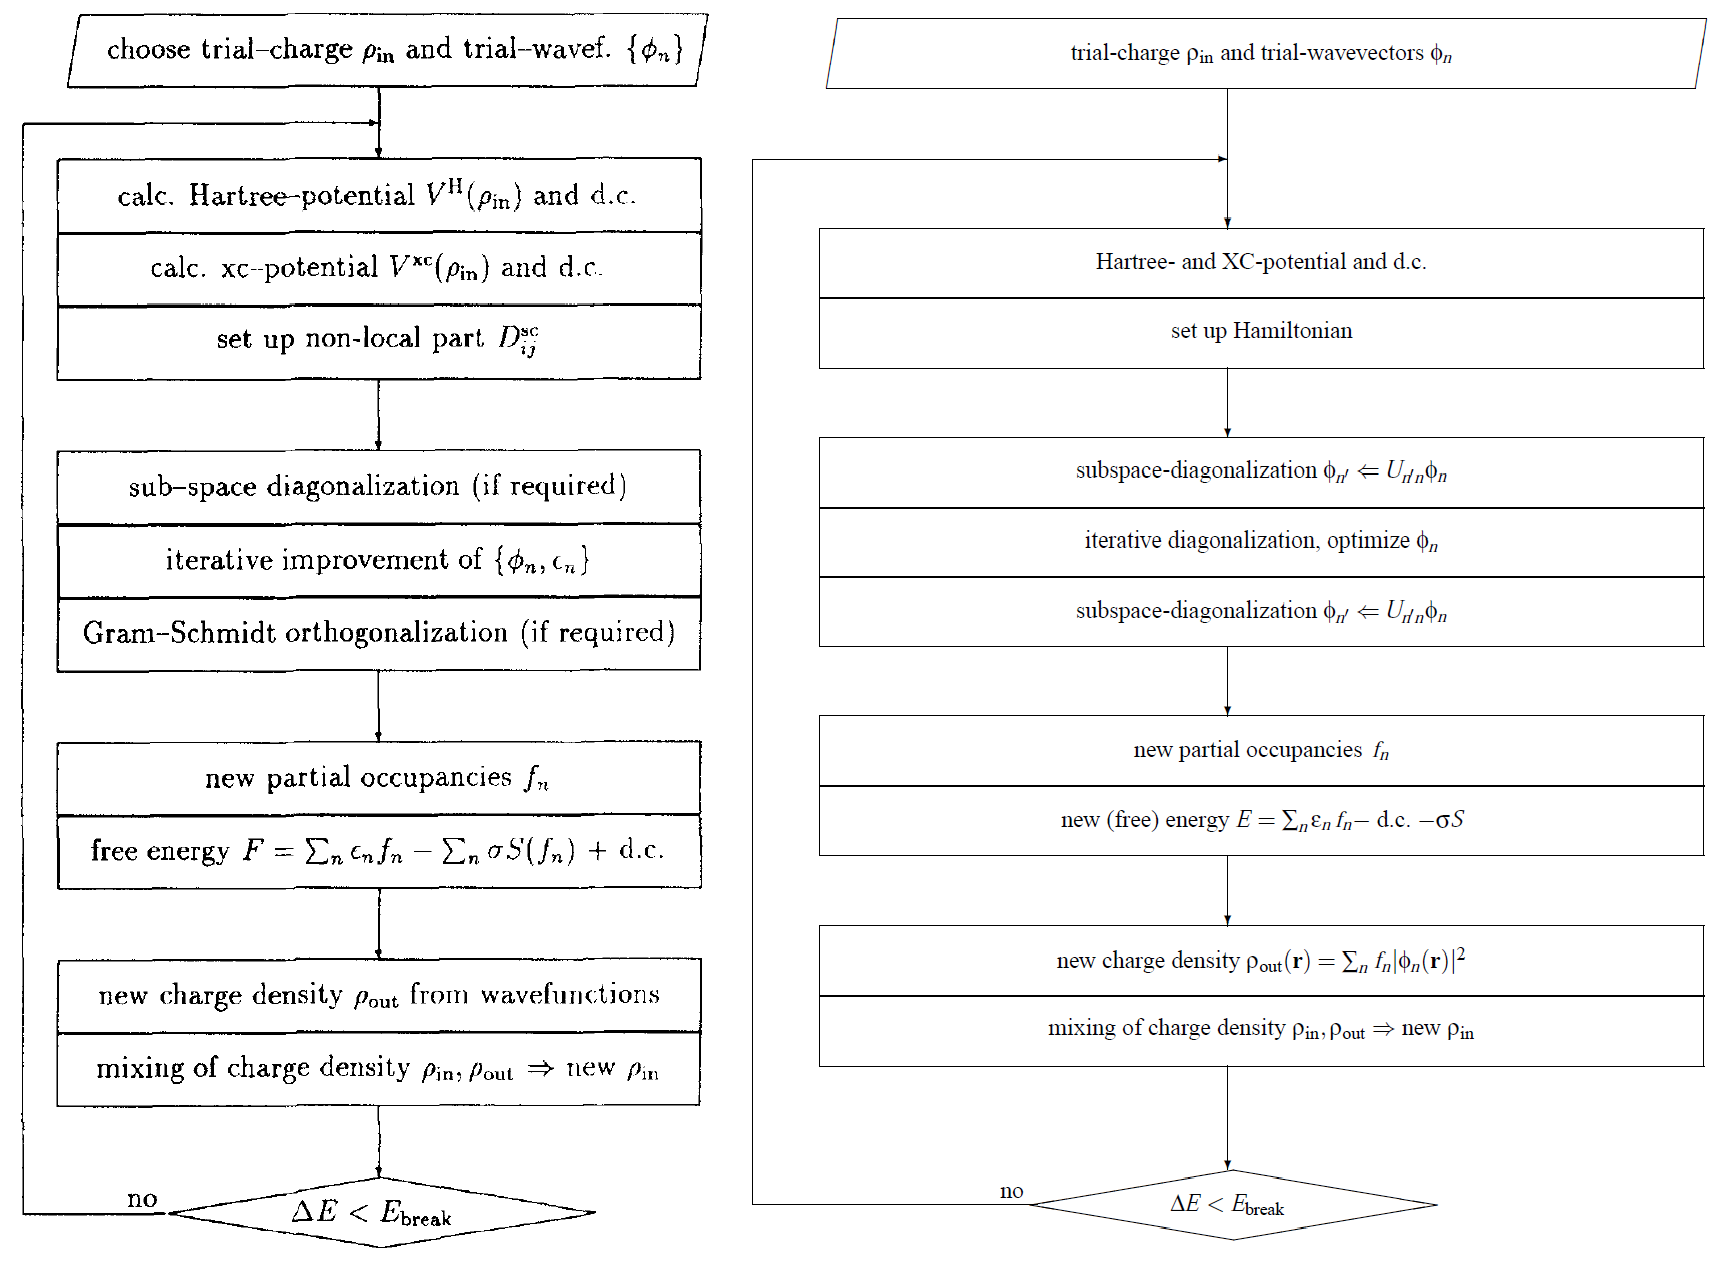
\includegraphics[height=2.7in,width=4.0in,viewport=0 0 1300 960,clip]{Figures/VASP_procedure-full.png}
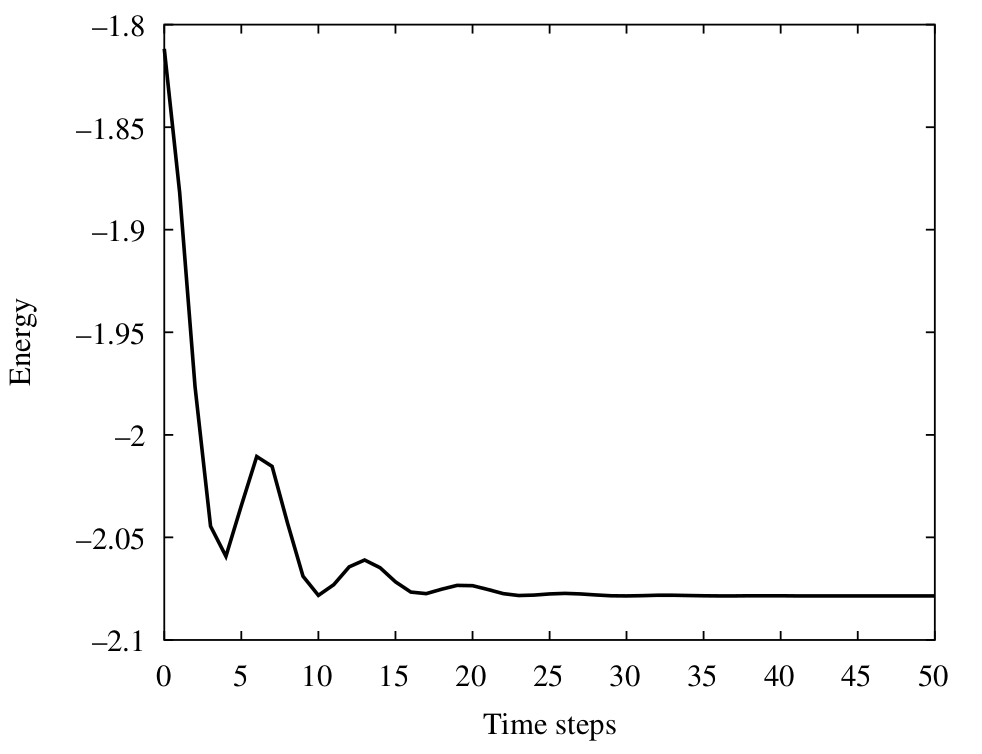
\includegraphics[height=1.5in,width=1.9in,viewport=0 0 740 600,clip]{Figures/Ab-initio-Ene.png}\\
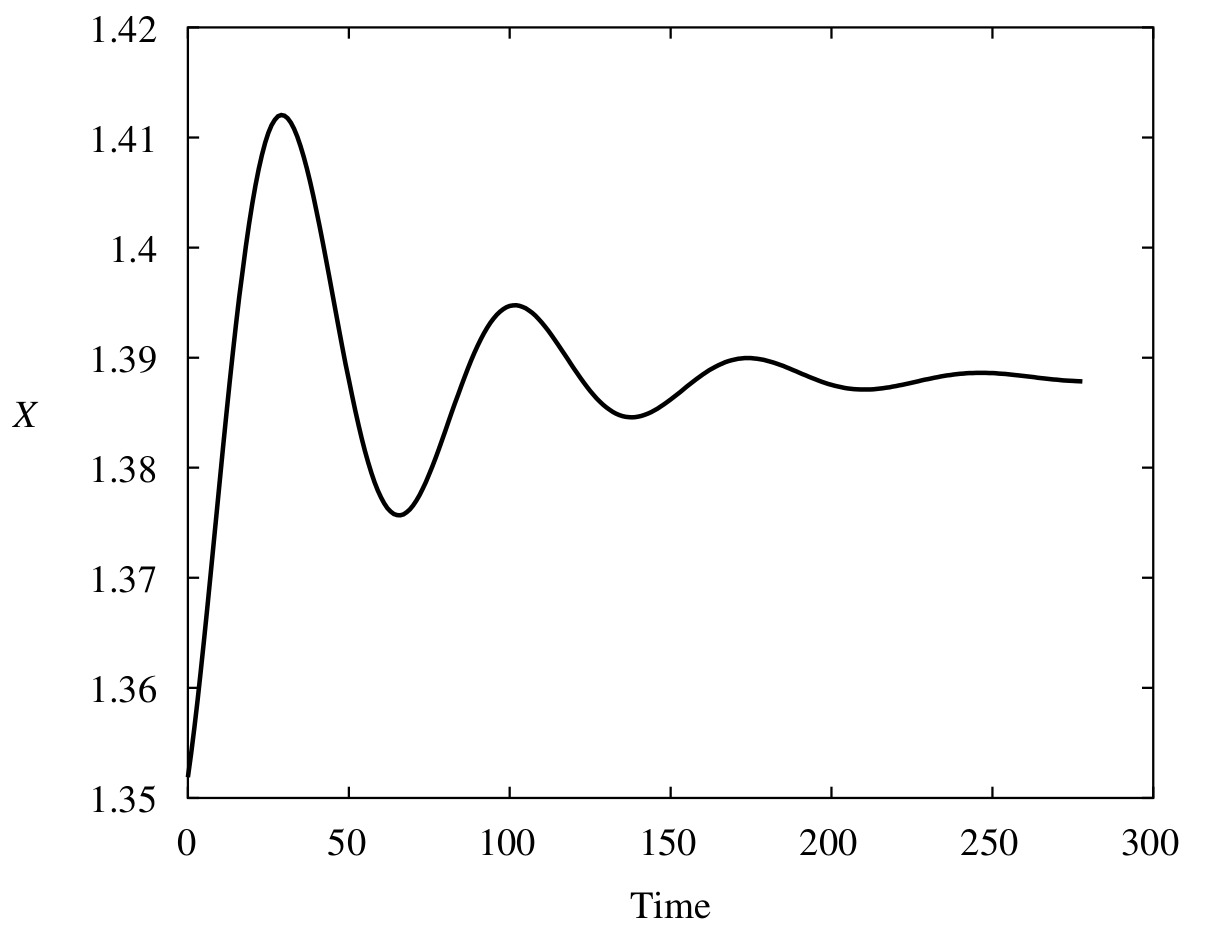
\includegraphics[height=1.5in,width=1.9in,viewport=0 0 1200 950,clip]{Figures/MD_H-R-rel.png}
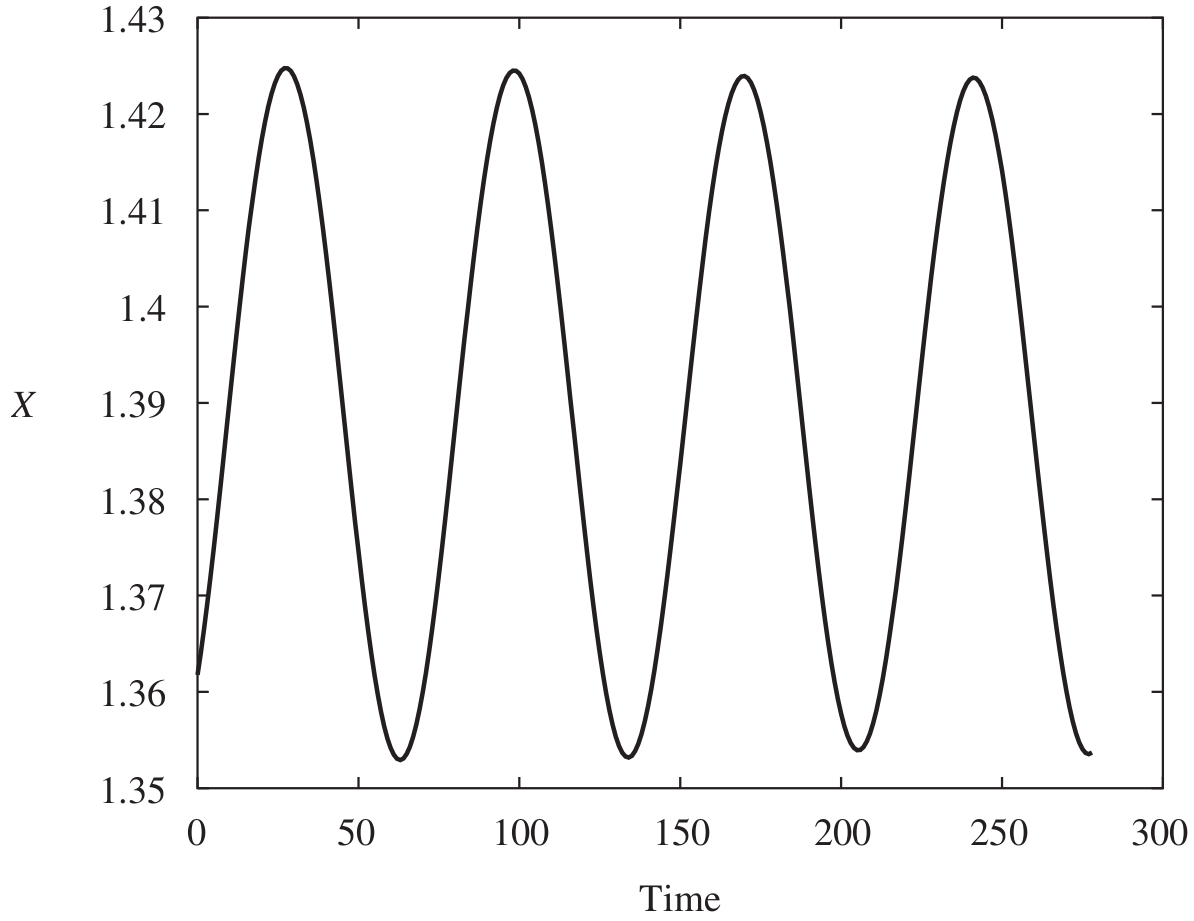
\includegraphics[height=1.5in,width=1.9in,viewport=0 0 1200 950,clip]{Figures/MD_H-R-MD.png}
\caption{\tiny \textrm{The Flow of calculation for the AIMD.}}%(与文献\cite{EPJB33-47_2003}图1对比)
\label{PAW_AIMD}
\end{figure} 
}


\frame
{
	\frametitle{波函数正交对计算的影响}
	{\fontsize{9.0pt}{5.2pt}\selectfont
	\textrm{Verlet}算法计算电子态波函数的运动方程
	\begin{displaymath}
		|\tilde\psi_k(t+h)\rangle=2|\psi_k(t)\rangle-|\psi_k(t-h)\rangle-\dfrac{2h^2}{\mu}(H|\psi_k(t)\rangle-\sum_l\Lambda_{kl}\psi_l)
	\end{displaymath}}
	当体系含有多个电子,\textrm{Langrage}乘子确保电子波函数彼此正交\\%,可有
	{\fontsize{7.0pt}{5.2pt}\selectfont
	实际上,存在多种正交方案
	\begin{itemize}
		\item 一次\textrm{unitary}变换产生一套正交轨道
			\begin{displaymath}
				\psi_k^{\prime}=\sum_lU_{kl}\psi_l
			\end{displaymath}
			这里基组$\{\psi_k^{\prime}\}$是正交的
		\item 一次波函数的\textrm{unitary}变化伴随\textrm{Lagtange}乘子的一次类似变换
			\begin{displaymath}
				\Lambda_{kl}^{\prime}=\sum_{mn}U_{km}^{\dagger}\Lambda_{mn}U_{nl}
			\end{displaymath}
	\end{itemize}
	不同的正交方案对应张开的空间相同,但张开空间的函数有所旋转
%	\begin{displaymath}
%		|\psi_k(t+h)\rangle=|\tilde\psi_k(t+h)\rangle+\sum_lX_{kl}|\psi_l(t)\rangle
%	\end{displaymath}
}\\
%	其中,{\fontsize{9.0pt}{5.2pt}\selectfont$X_{kl}=\dfrac{2h^2}{\mu}\Lambda_{kl}$},由此$|\psi_k(t+h)\rangle$正交\\
%	$X_{ij}$要求关于$\mathbf{X}$的矩阵方程
	{\fontsize{8.0pt}{5.2pt}\selectfont
	\textcolor{purple}{不同的旋转方式(不同的正交方案)会对\textrm{Verlet}算法的执行效率产生很大的影响}
%	\begin{displaymath}
%		\mathbf{X}\mathbf{X}^{\dag}+\mathbf{X}\mathbf{B}+\mathbf{B}^{\dag}\mathbf{X}^{\dag}=\mathbf{I}-\mathbf{A}
%	\end{displaymath}
}
%	能通过以下迭代快速收敛,这里{\fontsize{9.0pt}{5.2pt}\selectfont$A_{kl}=\langle\tilde\psi_k(t+h)|\tilde\psi_l(t+h)\rangle$},{\fontsize{9.0pt}{5.2pt}\selectfont$B_{kl}=\langle\psi_k(t)|\tilde\psi_l(t+h)\rangle$}
	{\fontsize{9.0pt}{5.2pt}\selectfont
%	\begin{displaymath}
%		\mathbf{X}^{(n+1)}=\frac12[\mathbf{I}-\mathbf{A}+\mathbf{X}^{(n)}(\mathbf{I}-\mathbf{B})+\mathbf{X}^{(n)}(\mathbf{I}-\mathbf{B}^{\dag})-\mathbf{X}^{n}\mathbf{X}^{(n){\dag}}]
%		\end{displaymath}
}
%	取初始{\fontsize{9.0pt}{5.2pt}\selectfont$\mathbf{X}=\frac12(\mathbf{I}-\mathbf{A})$}
}

%\subsection{电子态能量的最小化}
\frame[allowframebreaks]
{
	\frametitle{\textrm{CPMD}与平面波基}
	\begin{itemize}
		\item 推导总能对轨道自由度的受力
	{\fontsize{6.2pt}{5.2pt}\selectfont{
			\begin{displaymath}
				\begin{aligned}
					\dfrac{\partial E_{\mathrm{total}}}{\partial c_j^{\ast}(\vec K)}=&\dfrac{K^2}2c_j(\vec K)+\sum_{\vec K^{\prime}}V_{\mathrm{loc}}^{\ast}(\vec K-\vec K^{\prime})c_j(\vec K^{\prime})\\
					&+\sum_n\sum_{lm}F_{jlm}^n\mathrm{e}^{-\mathrm{i}\vec K\cdot\vec R_n}Y_{lm}(\hat{\vec K})h_{lm}^np_m^l(K)
				\end{aligned}
			\end{displaymath}
			这里$V_{\mathrm{loc}^{\mathrm{all}}}$是总局域势
			\begin{displaymath}
				V_{loc}(\vec K)=\sum_n\Delta V_{\mathrm{loc}}(\vec K)+V_{\mathrm{xc}}(\vec K)+4\pi\dfrac{n_{\mathrm{tot}}(\vec K)}{K^2}
			\end{displaymath}
		}}
		\item 推导总能对原子核的受力:\\
{\fontsize{6.2pt}{5.2pt}\selectfont{
			总能对原子位置坐标的梯度包括
			\begin{itemize}
{\fontsize{6.2pt}{5.2pt}\selectfont{
				\item 局域赝势部分的贡献
					\begin{displaymath}
						\nabla_{\vec R_n}E_{\mathrm{local}}=-\Omega\sum_{\vec K}\mathrm{i}\vec KV_{\mathrm{local,n}}(\vec K)\mathrm{e}^{-\mathrm{i}\vec K\cdot\vec R_n}n^{\ast}(\vec K)
					\end{displaymath}
				\item 非局域赝势部分的贡献
					\begin{displaymath}
						\nabla_{\vec R_n}E_{\mathrm{nonlocal}}=\sum_jf_j\sum_{l,m\varepsilon n}[(F_{jlm}^n)^{\ast}h_{lm}^n\nabla_{\vec R_n}F_{jlm}^n+\nabla_{\vec R_n}(F_{lm}^n)^{\ast}h_{lm}^nF_{lm}^n]
					\end{displaymath}
				\item 电子-核静电相互作用部分的贡献
					\begin{displaymath}
						\nabla_{\vec R_n}E_{\mathrm{ES}}=-\Omega\sum_{\vec K}\mathrm{i}\vec K\dfrac{n_{\mathrm{tot}}}{K^2}n_{\mathrm{core}}^n(\vec K)\mathrm{e}^{-\mathrm{i}\vec K\cdot\vec R_n}+\nabla_{\vec R_n}E_{\mathrm{ovrl}}
\end{displaymath}
				}}
			\end{itemize}
			其中
			\begin{displaymath}
				\nabla_{\vec R_n}F_{lm}^n=-\dfrac1{\sqrt{\Omega}}\sum_{\vec K}\mathrm{i}\vec K\mathrm{e}^{-\mathrm{i}\vec K\cdot\vec R_n}c_j^{\ast}(\vec K)Y_{lm}(\hat{\vec K})p_{lm}^l(\vec K)
			\end{displaymath}
			\begin{displaymath}
				\begin{aligned}
					\nabla_{\vec R_n}E_{\mathrm{ovrl}}=&\sideset{}{^{\prime}}\sum_{n^{\prime}}\sum_{\vec L}\bigg\{\dfrac{Z_nZ_{n^{\prime}}}{|\vec R_n-\vec R_{n^{\prime}}-\vec L|^3}\mathrm{erfc}\bigg[\dfrac{|\vec R_n-\vec R_{n^{\prime}}-\vec L|}{\sqrt{2(\xi_n^2+\xi_{n^{\prime}}^2)}}\bigg]\\
					&+\dfrac2{\sqrt{\pi}}\dfrac1{\sqrt{\xi_n^2+\xi_{n^{\prime}}^2}}\dfrac{Z_nZ_{n^{\prime}}}{|\vec R_n-\vec R_{n^{\prime}}-\vec L|^2}\mathrm{exp}\bigg[\dfrac{|\vec R_n-\vec R_{n^{\prime}}-\vec L|}{\sqrt{2(\xi_n^2+\xi_{n^{\prime}}^2)}}\bigg]\bigg\}\\
					&\times(\vec R_n-\vec R_{n^{\prime}}-\vec L)
				\end{aligned}
			\end{displaymath}
		}}
	\end{itemize}

}

\frame
{
	\frametitle{\textrm{CPMD}方法总结}
	\textrm{Car-Parinello~}方法基本思想
	\begin{itemize}
		\item 只对原子核位置考虑受力$-\dfrac{\partial E_{\mathrm{tot}}}{\partial\vec R_n}$作用
		\item 电子结构是通过某种最小化方法确定能量泛函$E_{\mathrm{tot}}[\rho(\vec r)]$的极值得到,而非\textrm{Born-Oppenheimer}近似下的自洽迭代
		\item \textrm{Verlet}算法确定核位移过程中,并不要求在每一步核位移时,电子步充分弛豫到当前结构的基态
	\end{itemize}
	在\textrm{Car-Parinello}方法中,电子结构的计算变成经典的优化问题:~电子密度迭代过程中,约束条件下最小化问题
	\begin{itemize}
		\item 电子本征态波函数彼此正交约束下迭代对角化(内循环):\\
			\textcolor{blue}{子空间旋转}:~不同的正交化方法对迭代计算的影响
		\item 电荷密度混合过程中电荷数守恒约束(外循环)
			\begin{displaymath}
				\sum\limits_{j=0}^i a_j=1
			\end{displaymath}
	\end{itemize}
}

%\frame
%{
%	\frametitle{统计系综}
%	系综(\textrm{Ensembles})是在一定的宏观条件下,由大量微观粒子组成的性质和结构完全相同的、处于各种运动状态的、各自独立的系统整体的集合\footnote{\fontsize{4.2pt}{2.2pt}\selectfont{简言之,系综是系统的集合(\textcolor{magenta}{系统}:~宏观相同,微观不同)。}}。\\
%	应用\textrm{Verlet}算法,完成单粒子运动的数值积分,可以得到动力学体系的\textrm{Hamiltonian}对应的能量,进而应用统计力学的统计系综,获得宏观体系的物理量
%\begin{figure}[h!]
%\centering
%\vspace*{-0.20in}
%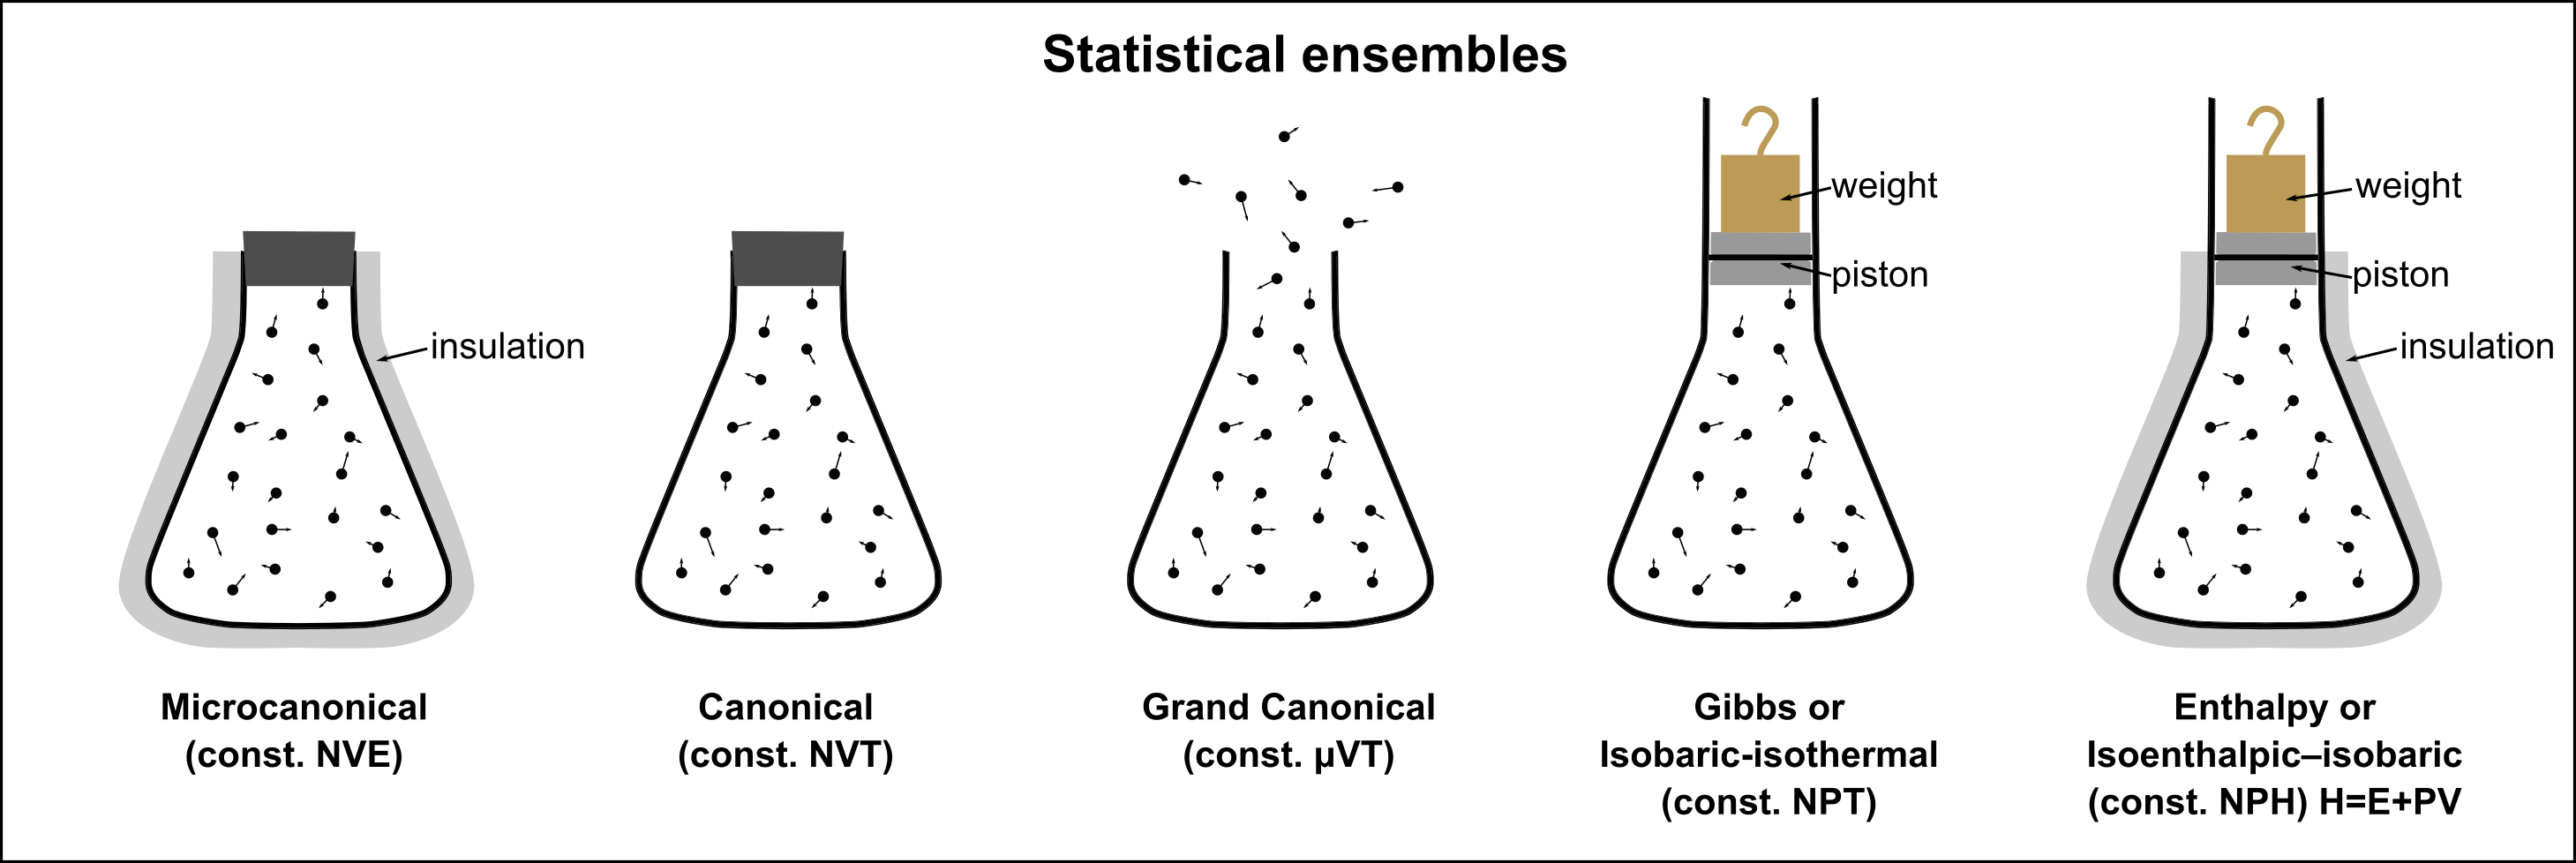
\includegraphics[height=1.60in,width=3.85in,viewport=0 0 1420 570,clip]{Figures/Statistical_Ensembles.png}
%%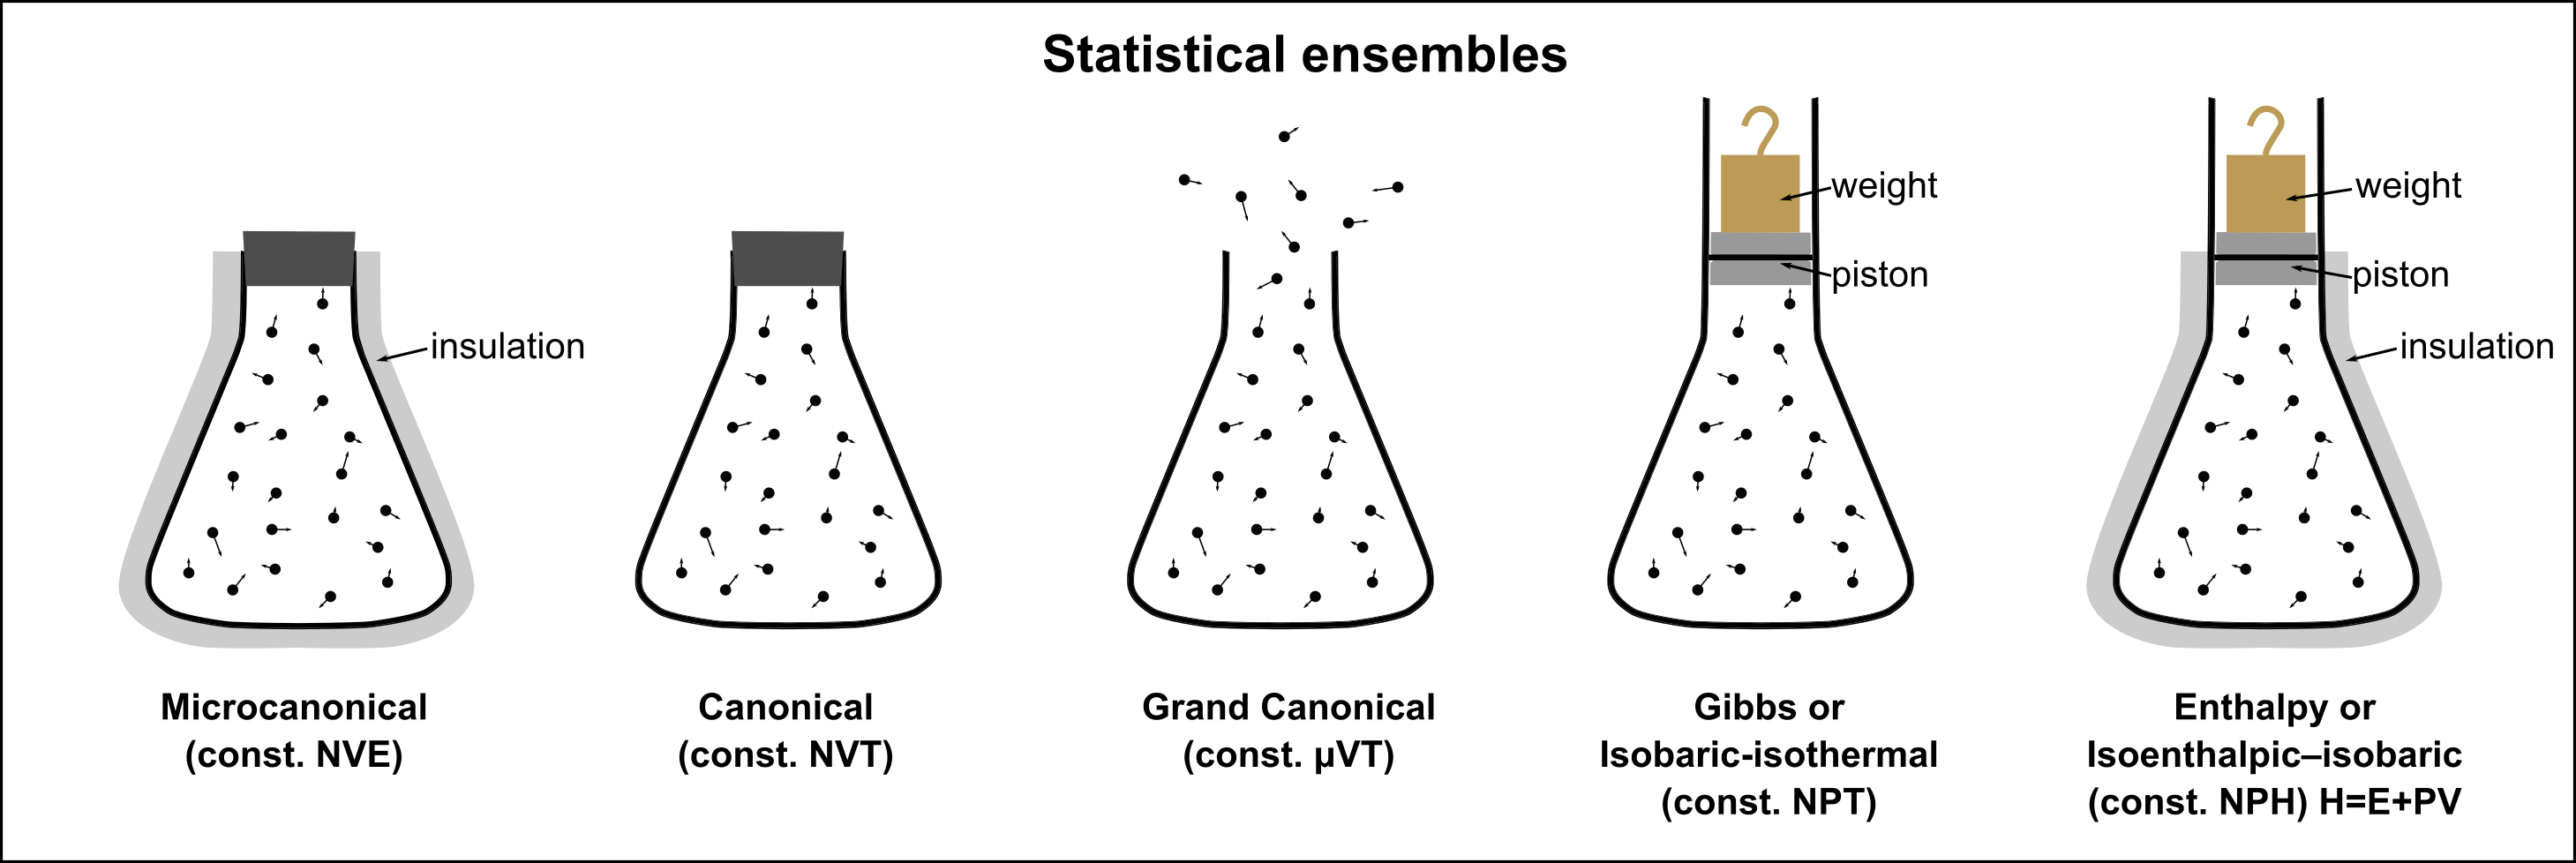
\includegraphics[height=1.30in,width=3.35in,viewport=0 0 1420 570,clip]{Figures/Statistical_Ensembles.png}
%%\caption{\tiny \textrm{The Statistical Ensembles.\footnote{\fontsize{3.5pt}{1.2pt}\selectfont{\textrm{canonical},汉译作“正则”,出自《楚辞\textperiodcentered 离骚》“皇揽揆余於初度兮,肇锡余以嘉名;~名余曰\textcolor{red}{正则}兮,字余曰灵均”,《楚辞章句》\upcite{Chucizhangju}:~“正,平也;~则,法也;~灵,神也;~均,调也。言正平可法则者,莫过于天;~养物均调者,莫过于地。高平曰原,故父伯庸名我为平以法天,字我为原以法地。言己上能安君,下能养民也。”,意思是说“正则”、“灵均”隐喻着某种意义,即平正是天的象征,原均是地的象征。因此正则的含义是“符合天道”,与\textrm{canonical}的意思\textrm{of, relating to, or forming a canon}意义一致。}}}}%(与文献\cite{EPJB33-47_2003}图1对比)
%\label{Statistical_Ensembles}
%\end{figure}
%}
%
%\frame
%{
%	\frametitle{第一原理分子动力学:~\textrm{CPMD}}
%	1985年\textrm{Car}和\textrm{Parrinello}在密度泛函理论基础上,将第一原理方法应用到分子动力学研究中,形成\textrm{Car-Parrinello Molecular dynamics~(CPMD)}
%	\begin{itemize}
%		\item 与\textrm{BOMD}不同,在\textrm{CPMD}中,电子自由度存在于经典\textrm{Lagrangian}中
%			\begin{displaymath}
%				\begin{aligned}
%					L_{\mathrm{CP}}(\{\psi_i\};~\mathbf{R},\dot{\mathbf{R}})=&\textcolor{blue}{\dfrac12\mu\sum_i\langle\dot{\psi}_i|\dot{\psi}_i\rangle}+\dfrac12\sum_{I=1}^NM_I\dot{\mathbf{R}}^2_I\\
%					-&\textcolor{red}{E}[\{\psi_i\};\mathbf{R}]\\
%					&+\sum_{ij}\Lambda_{ij}(\langle\psi_i|\psi_j\rangle-\delta_{ij})
%				\end{aligned}
%			\end{displaymath}
%			{\fontsize{6.2pt}{4.2pt}\selectfont{在经典\textrm{Lagrangian}中考虑电子自由度,人为地引入了傀电子质量参数$\mu$和傀轨道速度$\dot{\psi}_i$}}
%	\end{itemize}
%}
%
%\frame
%{
%	\frametitle{第一原理分子动力学:~\textrm{CPMD}}
%	\begin{itemize}
%		\item \textrm{CPMD}下的运动方程表示为
%			\begin{displaymath}
%				\begin{aligned}
%					M_I\ddot{\mathbf{R}}_I=&-\nabla_{\mathbf{R}_I}\bigg[E[\{\psi_i\};\mathbf{R}]\bigg|_{\{\langle\psi_i|\psi_j\rangle=\delta_{ij}\}}\bigg]\\
%					=&\textcolor{purple}{-\dfrac{\partial E}{\partial\mathbf{R}_I}}\textcolor{blue}{+\sum_{i,j}\Lambda_{ij}\dfrac{\partial}{\partial \mathbf{R}_I}\langle\psi_i|\psi_j\rangle}\\
%					\mu\ddot{\psi}_i(\vec r,t)=&-\dfrac{\delta E}{\delta\langle\psi_i|}+\sum_j\Lambda_{ij}|\psi_j\rangle\\
%					=&-\hat{H_{\mathrm{e}}}\langle\psi_j|+\sum_j\Lambda_{ij}|\psi_j\rangle
%				\end{aligned}
%			\end{displaymath}
%			{\fontsize{6.2pt}{4.2pt}\selectfont{$-\dfrac{\delta E}{\delta\langle\psi|}$表示经典力学框架下的电子受力,用来描述分子动力学范畴内电子自由度随原子核运动的情况 }}
%	\end{itemize}
%}

\frame
{
	\frametitle{\textrm{CPMD}计算的特点}
	\begin{itemize}
		\item 计算成本大大节约\\
			{\fontsize{8.2pt}{4.2pt}\selectfont{相比于\textrm{BOMD},\textrm{CPMD}无需在每个分子动力学时间步长执行电子自洽计算}}
		\item 计算时间步长不能太长\\
			{\fontsize{8.2pt}{4.2pt}\selectfont{绝热近似要求电子-核运动能量彼此分离,\textcolor{blue}{声子最高频率}$\omega_{\mathrm I}$必须远小于\textcolor{blue}{傀电子最低振动频率}$\omega_{\mathrm e}$
			\begin{displaymath}
				\omega_{\mathrm e}\propto\sqrt{\dfrac{\Delta E_{\mathrm{gap}}}{\mu}}
			\end{displaymath}
			$\Delta E_{\mathrm{gap}}$是\textrm{K-S}单粒子的带隙,许可最大时间步长$\Delta t_{\mathrm{max}}<1/\omega_{\mathrm{e}}$,大小主要由$\sqrt{\mu}$}}确定
		\item $\mu$物理上没有意义,但通过调节$\mu$可以平衡\textrm{AIMD}的效率和精度,一般选取$\mu$使得$\omega_{\mathrm{I}}<<\omega_{\mathrm{I}}$成立
		\item 对于金属/导体的\textrm{CPMD}计算,由于$\Delta E_{\mathrm{gap}}=0$,必须要求体系通过恒温条件平衡交换能或者泛函允许分数占据
		\end{itemize}
}

\frame
{
	\frametitle{其它\textrm{AIMD}:~\textrm{PIMD}和\textrm{Ehrenfest~MD}}
	\begin{itemize}
		\item \textrm{Path Integral~MD~(PIMD)}\footnote{\fontsize{6.2pt}{4.2pt}\selectfont{基于量子统计的第一原理路径积分称为\textrm{Feynman}路径积分\textrm{(path integrals)}}}\\
			\textrm{PIMD}用量子力学计算电子和原子核运动,因此该方法比\textrm{BOMD}和\textrm{CPMD}方法精确,特别是对于含有轻元素体系——计算量也要大得多
		\item \textrm{Ehrenfest~MD}\\
			电子自由度通过求解含时\textrm{(Time-dependent)~Schr\"odinger}方程得到,当$\Delta t\rightarrow0$,自由度变化对应于电子的幺正传播\textrm{(unitary propagation)}\footnote{\fontsize{6.2pt}{4.2pt}\selectfont{\textrm{Ehrenfest~MD}的幺正变换确保波函数保持正交,但代价是积分时间步长必须极小,因此\textrm{Ehrenfest~MD}模拟时间尺度仅达\textrm{atto}$(10^{-18})$秒尺度}}
	\end{itemize}
	\textcolor{blue}{\textrm{CPMD}结合了\textrm{BOMD}与\textrm{Ehrenfest~MD}的优点}:
	\begin{itemize}
		\item 计算体系受力由总能对粒子位置的求导,并非求电子态的$\langle\Psi_0|\hat H_{\mathrm{e}}|\Psi_0\rangle$极小值
		\item 因为选择平面波基,$\vec F_{\mathrm{NSC}}$自然为0
	\end{itemize}
}

\frame
{
	\frametitle{平衡态统计基础}
	系综(\textrm{Ensembles})是在一定的宏观条件下,由大量微观粒子组成的性质和结构完全相同的、处于各种运动状态的、各自独立的系统整体的集合。简言之,系综是给定宏观条件下,所有微观状态的集合。
%	应用\textrm{Verlet}算法,完成单粒子运动的数值积分,可以得到动力学体系的\textrm{Hamiltonian}对应的能量,进而应用统计力学的统计系综,获得宏观体系的物理量
	\vskip 3pt
	\textcolor{blue}{等概率原理}\textrm{(Principle of equal weights)}:\\
	一个热力学体系有相同的概率到达每个可能经历的微观态。\\
	等概率原理导出\textrm{Boltzmann}分布
	\begin{displaymath}
		P_j=\dfrac{\mathrm{e}^{-\beta\varepsilon_j}}Q
	\end{displaymath}
	这里$Q$称为配分函数\textrm{(partition function)}
	\begin{displaymath}
		\begin{aligned}
			Q=&\sum_i\mathrm{e}^{(-\beta\varepsilon_i)}\\
			\beta=&1/k_{\mathrm{B}}T
		\end{aligned}
	\end{displaymath}
	物理量的系综平均
	\begin{displaymath}
		\langle A\rangle=\sum_jA_j\mathrm{e}^{(-\beta\varepsilon_j)}/Q
	\end{displaymath}
}

\frame
{
	\frametitle{常用统计系综}
	{\fontsize{8.2pt}{4.2pt}\selectfont{应用\textrm{Verlet}算法,完成单粒子运动的数值积分,可以得到动力学体系的\textrm{Hamiltonian}对应的能量,基于统计系综,可获得体系的宏观物理量}}
\begin{figure}[h!]
\centering
\vspace*{-0.05in}
%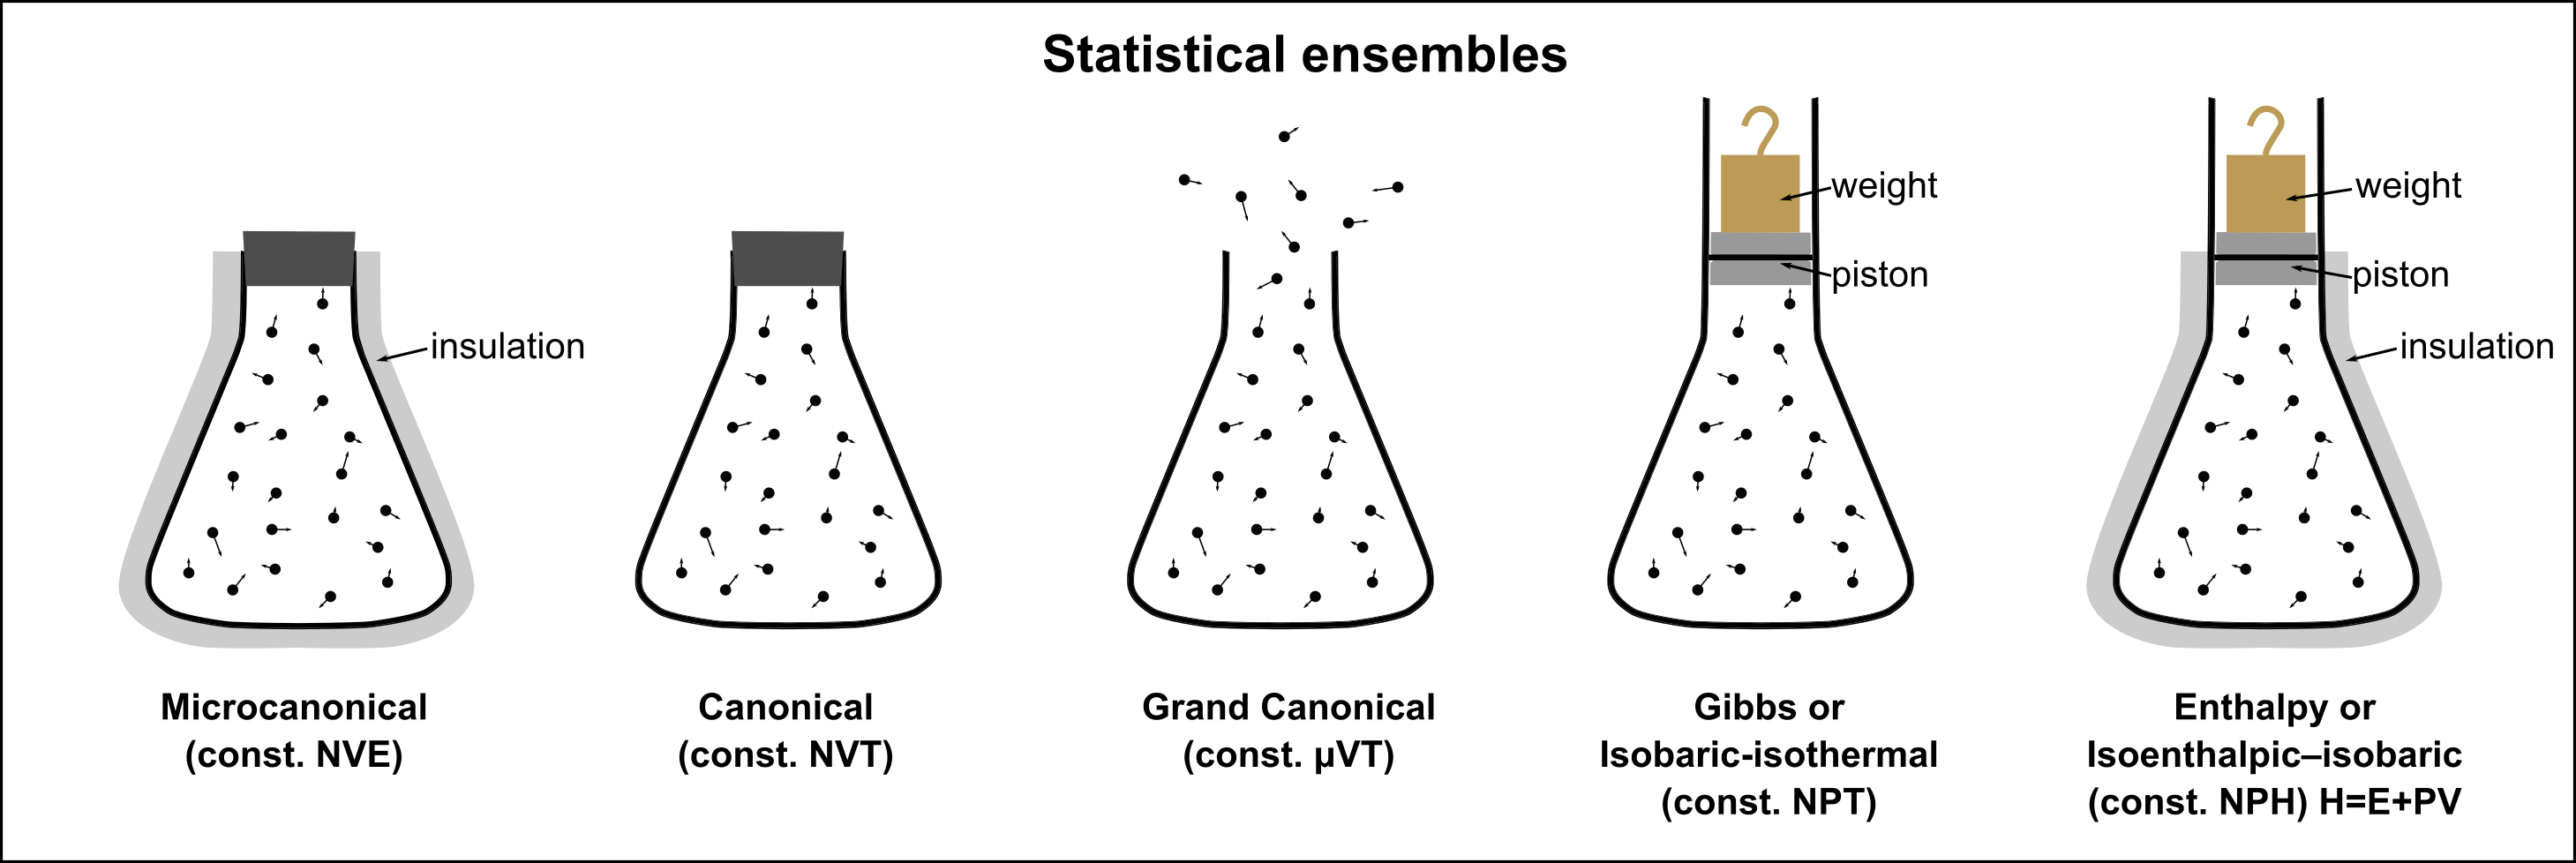
\includegraphics[height=1.60in,width=3.85in,viewport=0 0 1420 570,clip]{Figures/Statistical_Ensembles.png}
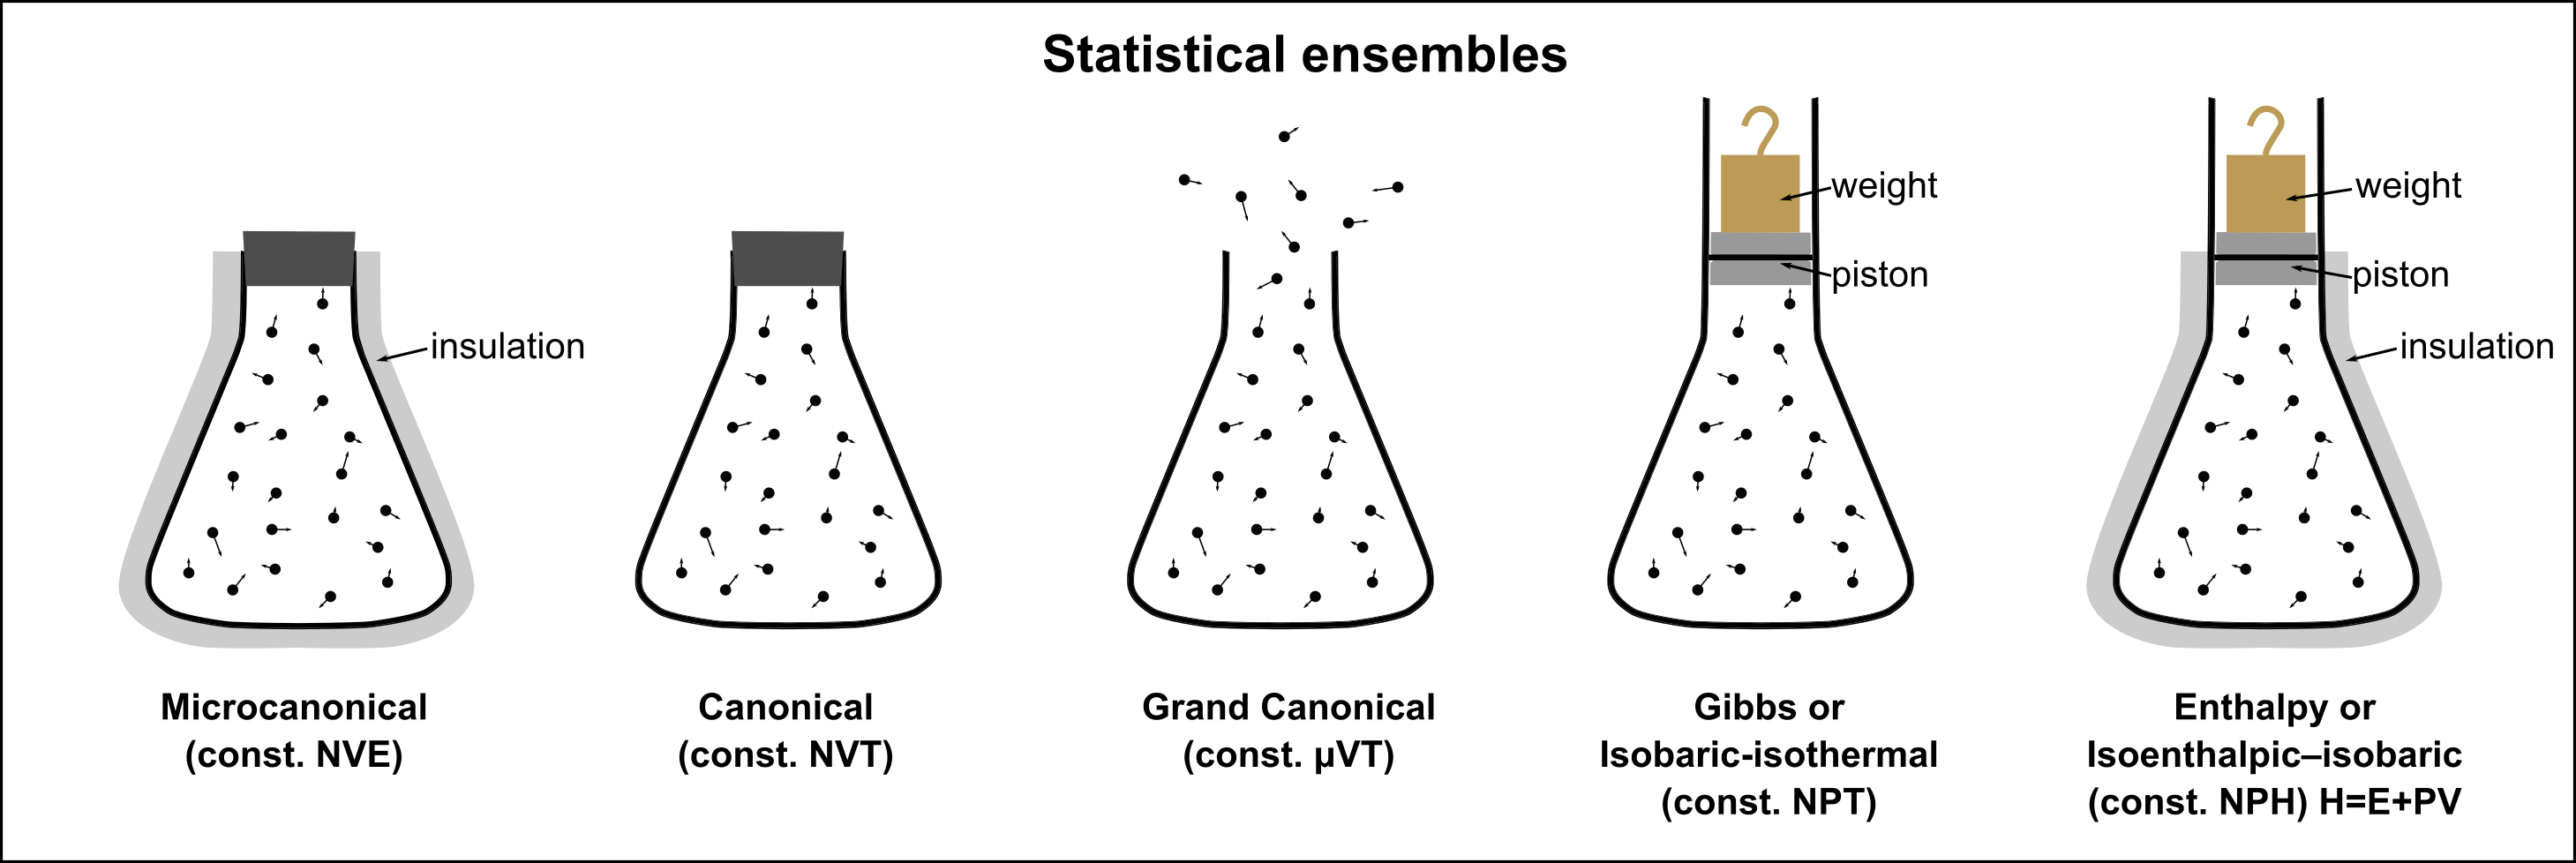
\includegraphics[height=1.20in,width=3.75in,viewport=0 0 1420 470,clip]{Figures/Statistical_Ensembles.png}
\caption{\tiny \textrm{The Statistical Ensembles.}}%(与文献\cite{EPJB33-47_2003}图1对比)
\label{Statistical_Ensembles}
\end{figure}
\vskip -15pt
\begin{itemize}
		{\fontsize{6.2pt}{1.2pt}\selectfont{
		\item 微正则系综\textrm{(Mircocanonical Ensemble)}%\footnote{\fontsize{4.5pt}{1.2pt}\selectfont{\textrm{canonical},汉译作``正则'',出自《楚辞\textperiodcentered 离骚》``皇揽揆余於初度兮,肇锡余以嘉名;~名余曰\textcolor{red}{正则}兮,字余曰灵均'',《楚辞章句》\upcite{Chucizhangju}:~``正,平也;~则,法也;~灵,神也;~均,调也。言正平可法则者,莫过于天;~养物均调者,莫神于地。高平曰原,故父伯庸名我为平以法天,字我为原以法地。言己上之能安君,下之能养民也。''意思是说``正则''、``灵均''隐喻着某种意义,即平正是天的象征,原均是地的象征。因此正则的含义是``\textcolor{blue}{符合天道}'',与\textrm{canonical}的意思\textrm{of, relating to, or forming a canon}意义一致。}}
			:~\textrm{NVE}皆为常数
		\item 正则系综\textrm{(Canonical Ensemble)}:~\textrm{NVT}皆为常数
		\item 巨正则系综\textrm{(Grandcanonical Ensemble)}:~\textrm{$\mu$VT}皆为常数,粒子数不固定
		\item 等压-等温系综\textrm{(Isobaric-Isothermal Ensemble)}:~\textrm{NPT}皆为常数
		\item 等焓-等压系综\textrm{(Isoenthalpic-Isobaric Ensemble)}:~\textrm{NPH}皆为常数
		\item 等张力-等温系综\textrm{(Isotension-Isothermal Ensemble)}:~容器形状可变 }}
\end{itemize}
}

\frame
{
	\frametitle{常用热力学量}
	\begin{itemize}
{\fontsize{7.8pt}{1.2pt}\selectfont{
		\item 动能 ~$E_{\mathrm{k}}=\bigg\langle\sum\limits_{i=1}^N\dfrac12m_iv_i^2\bigg\rangle$
		\item 势能 ~$E_{\mathrm{p}}=\bigg\langle\sum\limits_{i=1}^NE_{\mathrm{p}i}\bigg\rangle$
		\item 温度 ~$T=\dfrac1{\mathrm{d}Nk_{\mathrm{B}}}\bigg\langle\sum\limits_{i=1}^Nm_iv_i^2\bigg\rangle$ ~~~~ 其中$\mathrm{d}$是空间维度
		\item 压强 ~$p=\dfrac{k_{\mathrm{B}}TN}{V}+\dfrac1{\mathrm{d}V}\bigg\langle\sum\limits_{i<j}\vec f_{ij}\cdot\vec r_{ij}\bigg\rangle$
		\item 焓 ~$H=E+pV$ ~~~~ 相当于\textrm{NPT}下的有效总内能
		\item 熵 ~$S=k_{\mathrm{B}}\ln\Omega(N,V,E)$ ~~~~ $\Omega$是系统的总的微观状态数
		\item \textrm{Helmholtz}自由能:~\textcolor{blue}{\textrm{NVT}下的自由能}
			\begin{displaymath}
				F=E-TS=-k_{\mathrm{B}}T\ln{Q}
			\end{displaymath}
		\item \textrm{Gibbs}自由能:~\textcolor{blue}{\textrm{NPT}下的自由能}
			\begin{displaymath}
				G=F+pV=E-TS+pV
			\end{displaymath}
		\item 化学势 ~$\mu=\dfrac{\partial G}{\partial N}\bigg|_{T,p}=\dfrac{\partial F}{\partial N}\bigg|_{T,V}$}}
	\end{itemize}
}

\section{几何\rm{Berry~}相位}
\frame
{
	\frametitle{几何\textrm{Berry~}相位}
	\textrm{Berry}相位是一个复向量\textrm{(complex vector)}沿着参数空间中路径移动并回到起点所产生的全局相位演化\textrm{(global phase evolution)}
\begin{figure}[h!]
\centering
%\hspace*{-10pt}
\vspace*{-0.12in}
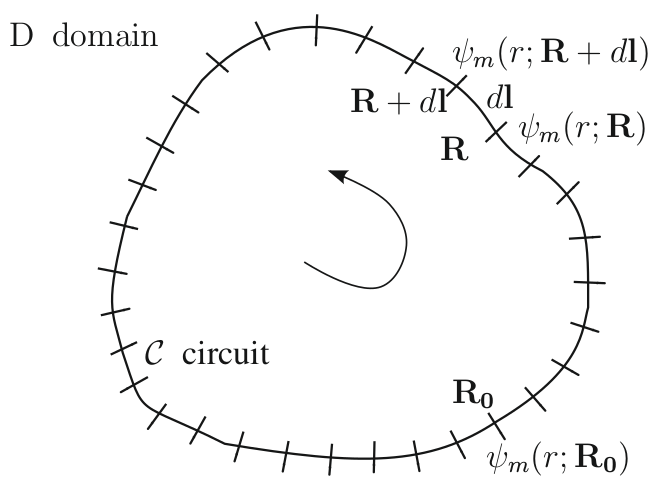
\includegraphics[height=1.8in,width=2.6in,viewport=0 0 800 540,clip]{Figures/Berry_Phase.png}
\caption{\tiny \textrm{Schematic representation of the sequence of states $\Psi_m(\vec r;\mathbf{R})$ as $\mathbf{R}$ is changed along a circuit \texttt{C} drawn in the parameter space D, where no degeneracy occurs.}}%
\label{Berry_Phase}
\end{figure} 
}

\frame
{
	\frametitle{\textrm{Berry~}相位的推导}
	一个包含若干参数$(R_1,R_2,\cdots)$的一般\textrm{Hamiltonian}~$H(\mathbf{R})$,这里用$\mathbf{R}$代表参数$(R_1,R_2,\cdots)$,即$\mathbf{R}=(R_1,R_2,\cdots)$\\
	本征态波函数$\psi_n(r;\mathbf{R})$和本征值$E_n(\mathbf{R})$满足\textrm{Schr\"odinger}方程
	\begin{displaymath}
		H(\mathbf{R})\psi_n(r;\mathbf{R})=E_n(\mathbf{R})\psi_n(r;\mathbf{R})
	\end{displaymath}
	不同参数$\mathbf{R}$下的本征值方程,不能唯一地确定波函数$\psi_n(r;\mathbf{R})$,因为在波函数$\psi_n(r;\mathbf{R})$中含有与$\mathbf{R}$相关的任意相位\footnote{\fontsize{6.0pt}{3.2pt}\selectfont{这种相位任意性称为\textcolor{blue}{规范任意性}(\textrm{gauge~abbitariness})。\textrm{gauge}最初是源于北美的一种关于直径的长度计量单位,属于布朗-夏普\textrm{(Brown \& Sharpe)}计量系统。物理学中的“\textrm{gauge}”有基准、参照的意思。}}

	在参数$\mathbf{R}$的定义域$D$内,假设波函数$\psi_n(r;\mathbf{R})$由一套连续、单值函数构成,有\textcolor{magenta}{规范变换}
	\begin{displaymath}
		\tilde{\psi}_n(r;\mathbf{R})=\mathrm{e}^{\mathrm{i}\alpha_n(\mathbf{R})}\psi_n(r;\mathbf{R})
	\end{displaymath}
	可以在参数定义域$D$内定义一套等价的连续、单值波函数,其中$\alpha_n(\mathbf{R})$是连续、单值的实函数

	\textcolor{blue}{\textrm{Berry}针对规范任意性,提出了规范不变性的几何相位计算过程}
}

\frame
{
	\frametitle{\textrm{Berry~}相位的推导}
\begin{figure}[h!]
\centering
%\hspace*{-10pt}
\vspace*{-0.25in}
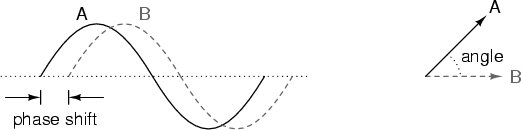
\includegraphics[height=1.2in,width=3.9in,viewport=0 0 125 35,clip]{Figures/complex_phase-shift.png}
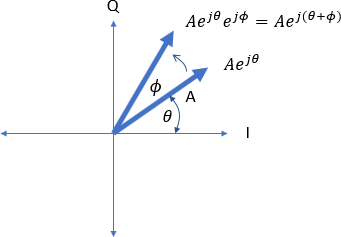
\includegraphics[height=1.6in,width=2.3in,viewport=0 0 360 240,clip]{Figures/complex_phase-difference.png}
\caption{\tiny \textrm{Schematic representation of the phase difference of wave vector in complex plane.}}%
\label{Complex-Phase-difference}
\end{figure} 
}

\frame
{
	\frametitle{\textrm{Berry~}相位的推导}
	在参数$\mathbf{R}$的定义域内,本征态波函数$\psi_n(r;\mathbf{R})$,对应的本征值$E_n(\mathbf{R})$,可以在不同层$n$间绝热变化。选择闭合回路$C$,如果回路上一点$\mathbf{R}$和临近点$\mathbf{R}+\mathrm{d}\mathbf{l}$的波函数分别为$\psi_n(r;\mathbf{R})$和$\psi_n(r;\mathbf{R}+\mathrm{d}\mathbf{l})$

	两个波函数的相位差(夹角)定义为
	\begin{displaymath}
		\mathrm{d}\phi\equiv\arg\langle\psi_n(r;\mathbf{R})|\psi_n(r;\mathbf{R}+\mathrm{d}\mathbf{l})\rangle
	\end{displaymath}
	$\mathrm{d}\phi$表示绝热层$n$中量子体系沿回路$C$由$\mathbf{R}$向$\mathbf{R}+\mathrm{d}\mathbf{l}$的相位无穷小的变化

	\textcolor{purple}{这样定义的$\mathrm{d}\phi$并没有明确的物理意义,因为$\mathrm{d}\phi$依赖于$\psi_n(r;\mathbf{R})$和$\psi_n(r;\mathbf{R}+\mathrm{d}\mathbf{l})$自身的相位}

	如果将$\psi_n(r;\mathbf{R}+\mathrm{d}\mathbf{l})$采用\textrm{Taylor}展开,并对$\mathrm{d}\mathbf{l}$近似到一阶有
	\begin{displaymath}
		\mathrm{d}\phi=\arg\bigg[1+\langle\psi_n(r;\mathbf{R})|\dfrac{\partial}{\partial\mathbf{R}}\psi_n(r;\mathbf{R})\rangle\cdot\mathrm{d}\mathbf{l}\bigg]
	\end{displaymath}
}

\frame
{
	\frametitle{\textrm{Berry~}相位的推导}
	在\textrm{Hellmann-Feynman}定理推导中,有表达式
	\textcolor{blue}{\begin{displaymath}
		\langle\psi_n(r;\mathbf{R})|\dfrac{\partial}{\partial\mathbf{R}}\psi_n(r;\mathbf{R})\rangle
	\end{displaymath}}
	为\textcolor{blue}{纯虚数},因此可有
	\begin{displaymath}
		\mathrm{d}\phi=\mathrm{Im}\langle\psi_n(r;\mathbf{R})|\dfrac{\partial}{\partial\mathbf{R}}\psi_n(r;\mathbf{R})\rangle\cdot\mathrm{d}\mathbf{l}
	\end{displaymath}
	\textcolor{purple}{闭合回路的相位演化,即\textrm{Berry~}相位,可表示为}
	\begin{displaymath}
		\gamma_n(C)=\mathrm{Im}\oint_C\langle\psi_n(r;\mathbf{R})|\dfrac{\partial}{\partial\mathbf{R}}\psi_n(r;\mathbf{R})\rangle\rangle\cdot\mathrm{d}\mathbf{l}
	\end{displaymath}
	记被积函数中虚部为
	\begin{displaymath}
		\mathbf{A}_n(\mathbf{R})=\mathrm{Im}\langle\psi_n(r;\mathbf{R})|\nabla_{\mathbf{R}}\psi_n(r;\mathbf{R})\rangle
	\end{displaymath}
	可有
	\begin{displaymath}
		\gamma_n(C)=\oint_C\mathbf{A}_n(\mathbf{R})\cdot\mathrm{d}\mathbf{l}
	\end{displaymath}
}

\frame
{
	\frametitle{\rm{Berry}相位的规范不变性}
	不难证明,围道积分中的\textcolor{blue}{被积函数是规范依赖的},但\textcolor{blue}{\textrm{Berry~}相位是规范不变的}
	\begin{displaymath}
		\begin{aligned}
			\tilde{\mathbf{A}}_n(\mathbf{R})=&\mathrm{Im}\langle\tilde{\psi}_n(r;\mathbf{R})|\nabla_{\mathbf{R}}\tilde{\psi}_n(r;\mathbf{R})\rangle\\
			=&\mathrm{Im}\langle\mathrm{e}^{\mathrm{i}\alpha_n(\mathbf{R})}\psi_n(r;\mathbf{R})|\nabla_{\mathbf{R}}\mathrm{e}^{\mathrm{i}\alpha_n(\mathbf{R})}\psi_n(r;\mathbf{R})\rangle\\
			=&\mathrm{Im}\langle\psi_n(r;\mathbf{R})|\nabla_{\mathbf{R}}\psi_n(r;\mathbf{R})\rangle+\nabla_{\mathbf{R}}\alpha_n(\mathbf{R})\\
			=&\mathbf{A}_n(\mathbf{R})+\nabla_{\mathbf{R}}\alpha_n(\mathbf{R})
		\end{aligned}
	\end{displaymath}
	因此
	\begin{displaymath}
		\tilde\gamma_n(C)=\oint_C\tilde{\mathbf{A}}_n(\mathbf{R})\cdot\mathrm{d}\mathbf{l}=\oint_C[\mathbf{A}_n(\mathbf{R})+\nabla_{\mathbf{R}}\alpha_n(\mathbf{R})]\cdot\mathrm{d}\mathbf{l}\textcolor{magenta}{\equiv\gamma_n(C)}
	\end{displaymath}
	因此最后一个等式成立:~\textcolor{blue}{\fontsize{8.2pt}{6.2pt}\selectfont{对单值函数$\alpha_n(\mathbf{R})$的梯度,闭合围道积分为零}}
\vskip 5pt
	利用\textrm{Stokes}定理,将闭合围道积分变换为表面积分,被积函数也将规范不变
}

\frame
{
	\frametitle{\rm{Berry}相位的规范不变性}
	在参数定义域$D$内,如果闭合围道$C$对应的曲面为$S$,根据\textrm{Stokes}定理有
	\begin{displaymath}
		\gamma_n(C)=\oint_C\mathbf{A}_n(\mathbf{R})\cdot\mathrm{d}\mathbf{l}=\int_S[\mathrm{curl}\mathbf{A}_n(\mathbf{R})]\mathrm{d}\mathbf{S}
	\end{displaymath}
	不难看出~$\mathrm{curl}\mathbf{A}_n(\mathbf{R})=\mathrm{curl}\tilde{\mathbf{A}}_n(\mathbf{R})$\\
	令
	\begin{displaymath}
		\mathbf{B}_n(\mathbf{R})=\mathrm{curl}\mathbf{A}_n(\mathbf{R})
	\end{displaymath}
	可导出
	\begin{displaymath}
		\begin{aligned}
			\mathbf{B}_n(\mathbf{R})=&\mathrm{Im}~\mathrm{curl}\langle\psi_n(r;\mathbf{R})|\nabla_{\mathbf{R}}\psi_n(r;\mathbf{R})\rangle\\
			=&\mathrm{Im}\langle\nabla_{\mathbf{R}}\psi_n(r;\mathbf{R})|\nabla_{\mathbf{R}}\psi_n(r;\mathbf{R})\rangle\\
			=&\mathrm{Im}\sideset{}{^{\prime}}\sum_{m}\langle\nabla_{\mathbf{R}}\psi_n(r;\mathbf{R})|\psi_m(r;\mathbf{R})\rangle\times\langle\psi_m(r;\mathbf{R})|\nabla_{\mathbf{R}}\tilde{\psi}_n(r;\mathbf{R})\rangle\\
		\end{aligned}
	\end{displaymath}
	求和仅包括全部$m\neq n$项
}

\frame
{
	\frametitle{\rm{Berry}相位的规范不变性}
	根据\textrm{Epstein}广义\textrm{Hellmann-Feynman}定理,对所有$m\neq n$
	\begin{displaymath}
		\hspace*{-10pt}
		\mathbf{B}_n(\mathbf{R})=\mathrm{Im}\sideset{}{^{\prime}}\sum_{m}\dfrac{\langle\psi_n(r;\mathbf{R})|\nabla_{\mathbf{R}}H|\psi_m(r;\mathbf{R})\rangle\times\langle\psi_m(r;\mathbf{R})|\nabla_{\mathbf{R}}H|\psi_n(r;\mathbf{R})\rangle}{[E_n(\mathbf{R})-E_m(\mathbf{R})]^2}
	\end{displaymath}
	并有
	\begin{displaymath}
		\gamma_n(C)=\int_S\mathbf{B}_n(\mathbf{R})\cdot\mathrm{d}\mathbf{S}
	\end{displaymath}
	\textrm{Berry~}相位可以视为$\mathbf{B}_n(\mathbf{R})$通过围道$C$对应表面的通量
\begin{figure}[h!]
\centering
%\hspace*{-10pt}
\vspace*{-0.05in}
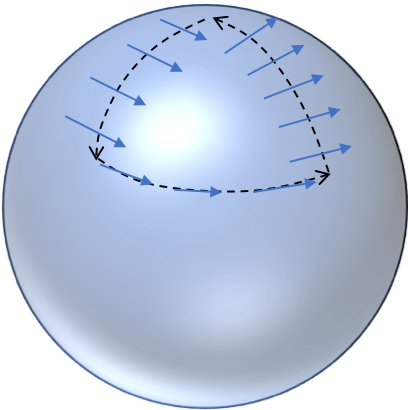
\includegraphics[height=1.1in,width=1.3in,viewport=0 0 500 420,clip]{Figures/Berry_Phase-2.png}
\caption{\tiny \textrm{The Berry phase $\gamma_n(C)$ can be interpreted as the flux of $\mathbf{B}_n(\mathbf{R})$ across a surface of contour $C$.}}%
\label{Berry-Phase-2}
\end{figure} 
}

\frame
{
	\frametitle{\rm{Berry}相位的规范不变性}
%	不难看出,根据$\mathbf{B}_n(\mathbf{R})$的定义其与电子波函数的相位无关\\
%	实际计算中通过$\mathbf{B}_n(\mathbf{R})来计算$\textrm{Berry~}的相位
%	\vskip 5pt
	$\mathbf{A}_n(\mathbf{R})$和$\mathbf{B}_n(\mathbf{R})$表现出与电磁理论中的物理量类似的特征:
	\begin{itemize}
		\item $\mathbf{A}_n(\mathbf{R})$类比于磁矢势\textrm{(magnetic vector potential)},称为\textcolor{blue}{\textrm{Berry}联络\textrm{(Berry~connection)}或\textrm{Berry potential}}\\
			\textcolor{red}{\textrm{Berry~}联络不是规范不变的}
		\item $\mathbf{B}_n(\mathbf{R})$类比于磁场\textrm{(magnetic field)},称为\textcolor{blue}{\textrm{Berry}曲率\textrm{(Berry~curvature)}}\\
			\textcolor{red}{\textrm{Berry~}曲率是规范不变的全反对二阶张量}
	\end{itemize}
	{\tiny \textrm{Berry~}曲率计算的讨论,也是证明\textrm{Chern}定理的关键
	\begin{displaymath}
		\oint_S\mathbf{B}_n(\mathbf{R})\cdot\mathrm{d}\mathbf{S}=2\pi C 
	\end{displaymath}
\begin{figure}[h!]
\centering
%\hspace*{-10pt}
\vspace*{-0.15in}
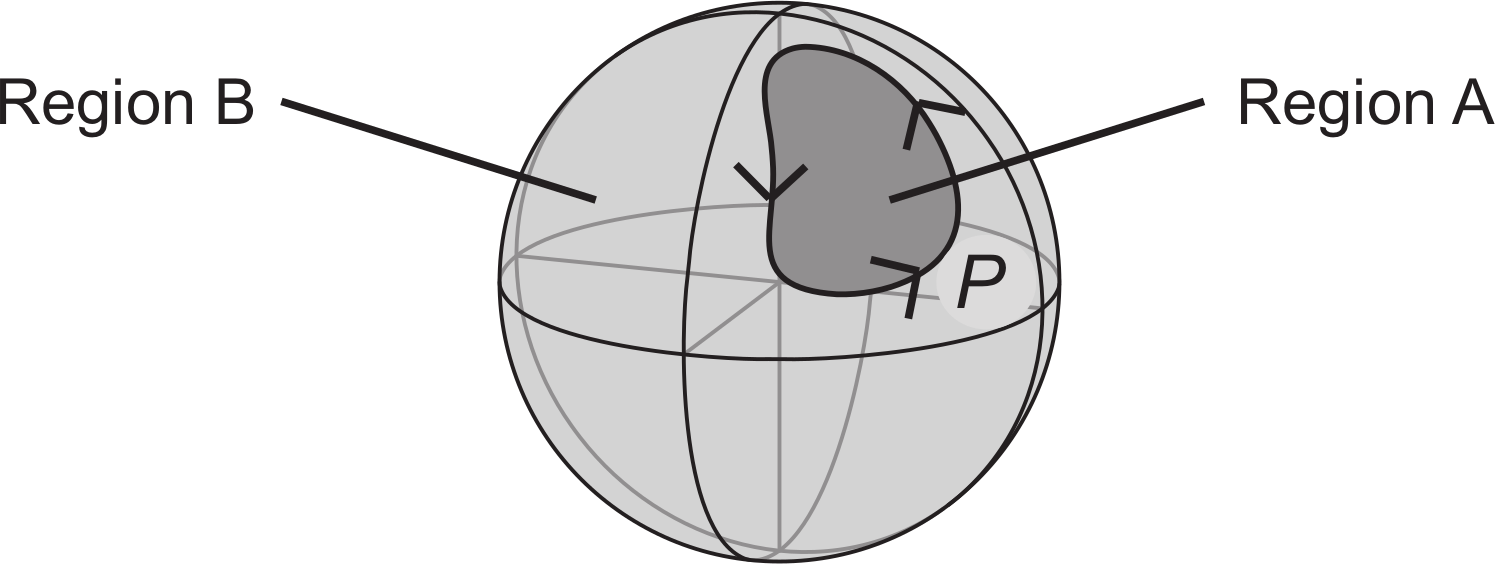
\includegraphics[height=0.7in,width=1.7in,viewport=0 0 1500 620,clip]{Figures/Berry-Phase_Chern.png}
\caption{\tiny \textrm{Proof of the Chern theorem for a manifold S having the topology of a sphere. Closed path $P$ traces the boundaries of subregions $A$ and $B$ in the forward and reverse directions respectively. The uniqueness modulo 2$π$ of the Berry phase around loop $P$ is the key to the proof.\cite{Berry-Phase}}}%
\label{Berry-Phase-Chern}
\end{figure}} 
}

\frame
{
	\frametitle{\rm{Bloch}表象与\rm{Berry~}相位}
	注意到\textrm{Bloch}函数的特征
	\begin{displaymath}
		\psi_n^{\vec k}(\vec r)=\mathrm{e}^{\mathrm{i}\vec k\cdot\vec r}u_n(\vec r)
	\end{displaymath}
	在计算\textrm{Berry~}相位时,\textcolor{blue}{必须使用周期函数$u_n(\vec r)$}:
	\begin{displaymath}
		\hspace*{-5pt}
		\langle\psi_n^{\vec k}|\psi_n^{\vec k+\vec b}\rangle=\int_{-\infty}^{+\infty}\mathrm{d}x\psi_n^{\vec k\ast}(x)\psi_n^{\vec k+\vec b}(x)=\int_{-\infty}^{+\infty}\mathrm{d}x\mathrm{e}^{\mathrm{i}bx} u_n^{\ast}(x)u_n(x)\textcolor{red}{=0}
	\end{displaymath}
而周期函数则有
	\begin{displaymath}
		\langle u_n|u_n\rangle=\int_0^a\mathrm{d}x u_n^{\ast}(x)u_n(x)
	\end{displaymath}
周期函数满足归一化条件
	\begin{displaymath}
		\langle u_n|u_n\rangle=\int_0^a\mathrm{d}x u_n^{\ast}(x)u_n(x)=1
	\end{displaymath}
}

\frame
{
	\frametitle{\rm{Bloch}表象与\rm{Berry~}相位}
	在\textrm{Bloch}表象下
	\begin{itemize}
		\item \textrm{Berry~}联络	
	\begin{displaymath}
		\mathbf{A}_n(k)=\langle u_{nk}|\mathrm{i}\nabla_{k}u_{nk}\rangle
	\end{displaymath}
\item \textrm{Berry~}曲率
	\begin{displaymath}
		\mathbf{B}_{n,\mu\nu}(k)=\partial_{\mu}\mathbf{A}_{n,\mu}(k)-\partial_{\nu}\mathbf{A}_{n,\nu}(k)=-2\mathrm{Im}\langle\partial_{\mu}u_{nk}|\partial_{\nu}u_{nk}\rangle
	\end{displaymath}
\item \textrm{Berry~}相位
	\begin{displaymath}
		\phi_n=\oint\mathbf{A}_n(k)\mathrm{d}k
	\end{displaymath}
	\end{itemize}
	在二维$\vec k$空间内,\textrm{Brillouin}区是圆环\textrm{(torus)},与能带$n$对应的陈数\textrm{(Chern number)}是
	\begin{displaymath}
		C_n=\dfrac1{2\pi}\int_{\mathrm{BZ}}\mathrm{d}k^2\mathbf{B}_{n,xy}
	\end{displaymath}
}

\frame
{
	\frametitle{\textrm{Berry~}曲率与晶格对称性}
	\begin{itemize}
		\item 晶格具有中心对称性\textrm{(Inversion~Symmetry)}
			\begin{displaymath}
				\mathbf{B}_n(\vec k)=\mathbf{B}(-\vec k)
			\end{displaymath}
		\item 晶格具有时间反演对称性\textrm{(Time-Reversal~Symmetry)}
			\begin{displaymath}
				\mathbf{B}_n(\vec k)=-\mathbf{B}(-\vec k)
			\end{displaymath}
		\item 晶格具有中心对称和时间反演对称性
			\begin{displaymath}
				\mathbf{B}_n(\vec k)=0
			\end{displaymath}
	\end{itemize}
}

\subsection{\rm{Wannier function}}
\frame
{
	\frametitle{\textrm{Wannier~}函数}
	\begin{itemize}
		\item \textrm{Wannier}函数是\textcolor{blue}{正交化的局域函数},\textcolor{red}{要求局域函数空间与能带空间完全相同}
		\item 紧束缚近似下,能带的电子波函数的\underline{\textcolor{blue}{\textrm{Bloch~}和}}
			\begin{displaymath}
				\psi_i^{\vec k}(\vec r)=\frac1{\sqrt N}\sum_m\mathrm{e}^{\mathrm{i}\vec k\cdot\vec R_m}\phi_i(\vec r-\vec R_m)
			\end{displaymath}
		\textrm{Bloch~}函数可以写类似形式
		\begin{displaymath}
			\psi_i^{\vec k}(\vec r)=\frac1{\sqrt N}\sum_m\mathrm{e}^{\mathrm{i}\vec k\cdot\vec R_m}w_i(\vec r-\vec R_m) 
		\end{displaymath}
		这里$w_i(\vec r-\vec R_n)$就是\textrm{Wannier~}函数
	\end{itemize}
}

\frame
{
	\frametitle{\textrm{Wannier~}函数}
	\begin{itemize}
		\item \textrm{Wannier~}函数是\textrm{Bloch~}函数的\textrm{Fourier}变换,对于格点$\vec T_m$有
			\begin{displaymath}
				\begin{aligned}
					&w_i(\vec r-\vec T_m)=\frac{\Omega_{\mathrm{cell}}}{(2\pi)^3}\int_{\mathrm{BZ}}\mathrm{d}\vec k\mathrm{e}^{-\mathrm{i}\vec k\cdot\vec T_m}\psi_i^{\vec k}(\vec r)\\
					=&\frac{\Omega_{\mathrm{cell}}}{(2\pi)^3}\int_{\mathrm{BZ}}\mathrm{d}\vec k\mathrm{e}^{-\mathrm{i}\vec k\cdot\vec T_m}\mathrm{e}^{-\mathrm{i}\vec k\cdot\vec r}u_i^{\vec k}(\vec r)=\frac{\Omega_{\mathrm{cell}}}{(2\pi)^3}\int_{\mathrm{BZ}}\mathrm{d}\vec k\mathrm{e}^{\mathrm{i}\vec k\cdot(\vec r-\vec T_m)}u_i^{\vec k}(\vec r)
				\end{aligned}
			\end{displaymath}
\begin{figure}[h!]
\centering
%\hspace*{-10pt}
\vspace*{-0.6in}
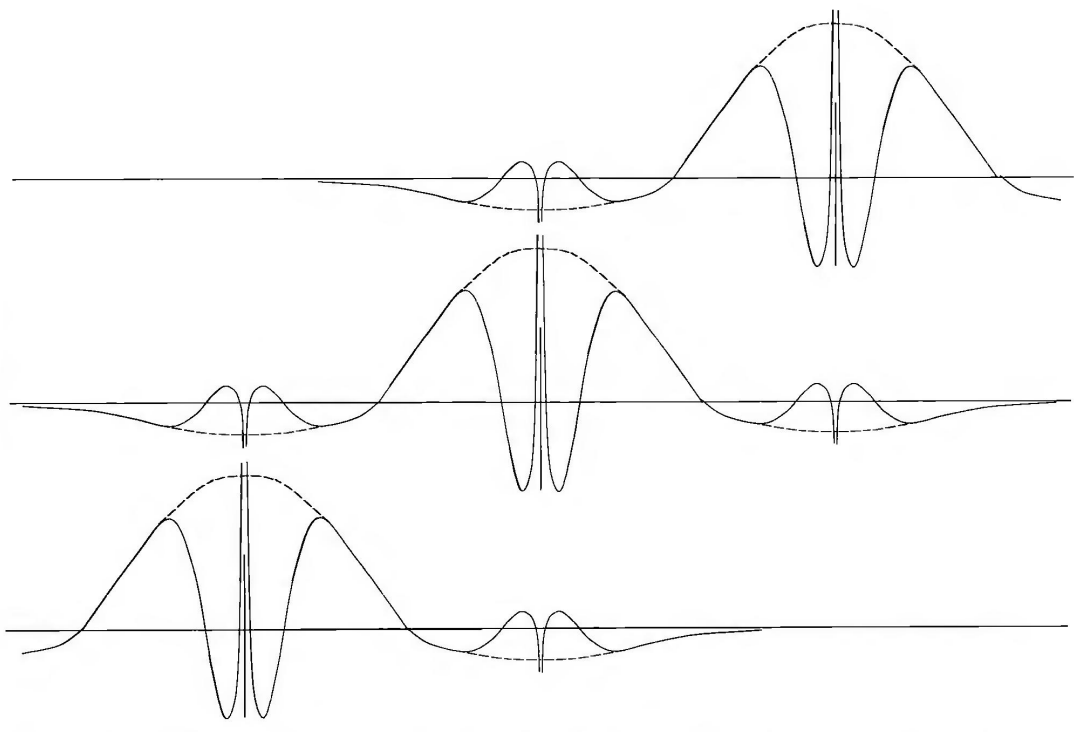
\includegraphics[height=1.8in,width=3.1in,viewport=0 0 1400 1000,clip]{Figures/Wannier_function.png}
\caption{\tiny \textrm{Schematic example of Wannier function that correspond to the Bloch function.}}%
\label{Wannier-function}
\end{figure} 
	\end{itemize}
}

\frame
{
	\frametitle{\textrm{Wannier~}函数}
	\begin{itemize}
		\item 一个能带的\textrm{Wannier~}函数完全由同一能带的\textrm{Bloch~}函数定义
		\item \textrm{Wannier~}函数完全正交
			\begin{displaymath}
				\int_{\textcolor{red}{\mathrm{all\; space}}}\mathrm{d}\vec rw_i^{\ast}(\vec r-\vec T_m)w_j(\vec r-\vec T_{m^{\prime}})=\delta_{ij}\delta_{mm^{\prime}}
			\end{displaymath}
			\textrm{Wannier~}函数和\textrm{Bloch~}函数一样,构成完备的正交函数集
		\item \textrm{Wannier~}函数在实空间内是局域的
			\begin{displaymath}
				\lim_{|\vec r-\vec R_n|\rightarrow\infty}|w_i(\vec r-\vec R_n)|=0
			\end{displaymath}
		\item \textrm{Wannier~}函数间由幺正矩阵联系
			\begin{displaymath}
				w_{i\vec k}=\sum_jU_{ji}^{\vec k}w_{j\vec k}^{(0)}
			\end{displaymath}
			\textcolor{blue}{其中$U_{ji}^{\vec k}$是与$\vec k$~关联的幺正矩阵},并满足平移周期性
\begin{displaymath}
	w_i(\vec r-\vec R_n)=w_i(\vec r-R_0)
\end{displaymath}
	\end{itemize}
}

\frame
{
	\frametitle{\textrm{Wannier~}函数的不唯一}
	\begin{itemize}
		\item 对于\textrm{Bloch~}函数
			\begin{displaymath}
				\psi_i^{\vec k}(\vec r)=\mathrm{e}^{\mathrm{i}\vec k\cdot\vec r}u_i^{\vec k}(\vec r)
			\end{displaymath}
			\textcolor{red}{可乘以任意相位,而不改变物理量的值}
			\begin{displaymath}
				\psi_i^{\vec k}(\vec r)\rightarrow\tilde\psi_i^{\vec k}(\vec r)=\textcolor{red}{\mathrm{e}^{\mathrm{i}\phi_i(\vec k)}}\psi_i^{\vec k}(\vec r)
			\end{displaymath}
		\item \textcolor{blue}{\textrm{Wannier~}函数的表示并不唯一}:\\
必须通过选择特定的相位$\phi_i(\vec k)$(或特定的幺正变换矩阵),才能得到确定的\textrm{Wannier~}函数 
\begin{figure}[h!]
\centering
%\hspace*{-10pt}
\vspace*{-0.2in}
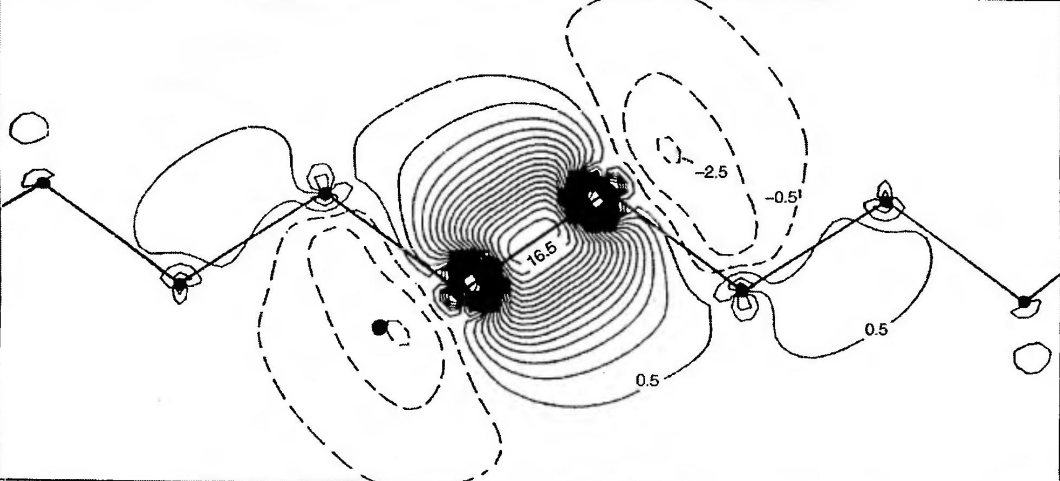
\includegraphics[height=1.1in,width=1.8in,viewport=0 0 1100 600,clip]{Figures/Wannier_function-Bondcenter_Si.png}
\caption{\tiny \textrm{Bond-centered Wannier function for Si.}}%
\label{Bond-Centered Wannier function}
\end{figure} 
	\end{itemize}
}

\frame
{
	\frametitle{\textrm{Wannier~}函数的不唯一}
\begin{figure}[h!]
\centering
\hspace*{-0.35in}
\subfigure[{\tiny \textrm{Maximally localized Wannier function}}]{
\label{Wannier-Maxlocal}
\vspace*{-0.50in}
\includegraphics[height=1.10in,width=3.20in,viewport=0 0 1000 450,clip]{Figures/Wannier_function-Maxlocal.png}}
\subfigure[{\tiny \textrm{Comparison of orthogonal and non-orthogonal maximally locaized orbitals}}]{
\label{Non_orth-Wannier}
\vspace*{-0.50in}
\includegraphics[height=1.10in,width=3.00in,viewport=0 0 1200 550,clip]{Figures/Non_orth-Wannier_function.png}}
\label{Non-local Wannier-function}
\end{figure}
}

\frame
{
	\frametitle{\textrm{Wannier~}表象下的能量与位置函数}
	\begin{itemize}
		\item \textrm{Wannier~}表象下\textrm{Hamiltonian}矩阵元是能带对角化的,并为能带$E_n(\vec k)$的\textrm{Fourier}变换的逆变换
			\begin{displaymath}
				\langle w_{n0}|H|w_{n\vec R}\rangle=E_{nR}
			\end{displaymath}
			\textrm{Wannier~}函数主要用于构建紧束缚模型\textrm{(tight-binding model)}\\
			$E_n(0)$和$E_n(\vec R)$分别对应格点在位能量\textrm{(on-site energy)}与跃迁能量\textrm{(hopping energy)}\\
			这也被称为\textrm{Wannier~}内插\textrm{(Wannier interpolation)}
		\item \textrm{Wannier~}表象下,位置算符的矩阵元是\textrm{Berry~}联络的\textrm{Fourier}逆变换
			\begin{displaymath}
				\langle w_{n0}|\vec r|w_{n\vec R}\rangle=\mathbf{A}_{n,\vec R}
			\end{displaymath}
	\end{itemize}
}

\frame
{
	\frametitle{\textrm{Wannier~}中心与\textrm{Berry~}相位}
	根据\textrm{Wannier~}函数中心\textrm{(Wannier center)}的定义,可有
			\begin{displaymath}
				\bar{\vec r}_n\equiv\langle w_{n0}|\vec r|w_{n0}\rangle=\dfrac{\Omega_{\mathrm{cell}}}{(2\pi)^3}\int\mathrm{d}\vec k\mathbf{A}_n(\vec k)
			\end{displaymath}
			\textcolor{blue}{不难看出,\textrm{Wannier~}中心是\textrm{Berry}联络在\textrm{Brillouin}区的平均}\\
	在一维条件下有
	\begin{displaymath}
		\bar{x}_n=\dfrac{a}{2\pi}\int_0^{2\pi}\mathrm{d}k\langle u_{nk}|\mathrm{i}\partial_{k}u_{nk}\rangle=a\dfrac{\phi_n}{2\pi}
	\end{displaymath}
	表明\textcolor{blue}{\textrm{Berry~}相位从$0$到$2\pi$的演化,对应于\textrm{Wannier~}中心从$x=0$到$x=a$的迁移}
	\vskip 8pt
	\textcolor{purple}{一维情况下,\textrm{Berry~}相位的规范不变性(同余$2\pi$)要求\textrm{Wannier~}中心在连续演变时也保持规范不变性}
}

\subsection{现代极化理论与\rm{Berry~}相位}
\frame
{
	\frametitle{电介质材料的极化与\textrm{Berry~}相位}
	\textcolor{blue}{电极化}:~电介质内部正负电荷的相对位移,会形成电偶极,这现象称为电极化
	\begin{itemize}
\setlength{\itemsep}{10pt}
		\item \textcolor{red}{压电效应}:~\textcolor{blue}{电介质沿一定方向受外力发生形变时,内部会产生极化现象:~在电解质两个相对表面出现正负相反电荷;当作用力方向改变时,电荷的极性也随之改变;当外力去掉后,又会恢复到不带电的状态}
		\item \textcolor{red}{热电效应}:~\textcolor{blue}{电介质因为受热,电子(空穴)由高温区往低温区移动时,产生电荷堆积,引起极化}
		\item \textcolor{red}{铁电效应}:~\textcolor{blue}{某些电介质中,晶胞的结构使正负电荷中心不重合而出现电偶极矩,在内部产生非零的电极化矢量,使晶体具有自发极化,且电偶极矩方向可以因外电场而改变,呈现出类似于铁磁体的特点}
	\end{itemize}
}

\frame
{
	\frametitle{外电场下的极化}
	\begin{itemize}
		\item 金属在外电场下的极化
	\end{itemize}
\begin{figure}[h!]
\centering
%\hspace*{-10pt}
\vspace*{-0.15in}
\includegraphics[height=2.0in,width=3.1in,viewport=0 0 900 650,clip]{Figures/Polarize_metal-2.png}
\caption{\tiny \textrm{Schematic of a metal in the static electric field.}}%
\label{Polarization_metal}
\end{figure} 
\textcolor{blue}{金属体相的物理性质不会受外场的影响}
}

\frame
{
	\frametitle{外电场下的极化}
	\begin{itemize}
		\item 绝缘体在外电场下的极化\\
			根据电磁理论,电极化矢量的梯度可表示为
			\begin{displaymath}
				\nabla\cdot\vec P(\vec r,t)=-\delta n(\vec r,t)
			\end{displaymath}
			利用极化电流守恒条件$\nabla\cdot\mathbf{j}(\vec r,t)=-\mathrm{d}n(\vec r,t)/\mathrm{d}t$\\
			可得电极化矢量与极化电流密度关系
			\begin{displaymath}
				\frac{\mathrm{d}\vec P(\vec r,t)}{\mathrm{d}t}=\mathbf{j}(\vec r,t)+\nabla\times\mathbf{M}(\vec r,t)
			\end{displaymath}
			这里$\mathbf{M}(\vec r,t)$是任意矢量场

			宏观电极化矢量定义为:~\textcolor{blue}{单位体积内电偶极矩的矢量和}
\begin{displaymath}
	\vec P=\dfrac1{\Omega}\int_{V_{\Omega}}n_{\mathrm{tot}}(\vec r)\vec r\mathrm{d}\vec r
\end{displaymath}
	\end{itemize}
%	\textcolor{red}{对于周期体系,这样定义的极化强度存在一定的问题}
}

\frame
{
	\frametitle{外电场下的极化:~有限体系}
			\begin{enumerate}
				\item 对于有限体系,上述定义的电极化矢量是合理的
			\end{enumerate}
\begin{figure}[h!]
\centering
%\hspace*{-10pt}
\vspace*{-0.08in}
\includegraphics[height=0.9in,width=2.2in,viewport=0 0 1100 550,clip]{Figures/Polarize_insulator.png}
\caption{\tiny \textrm{Illustration of finite system for which the total dipole moment is well defined.}}%
\label{Polarization_insulator}
\end{figure} 
\fontsize{8.5pt}{2.2pt}\selectfont{对有限体系,当外部电场$\vec E(\vec r)=0$,宏观电极化矢量$\vec P$可用偶极矩$\vec d$表示}
\begin{displaymath}
	\vec P\equiv\frac{\sum\limits_{\Omega}\vec d_i}{\Omega}=\frac1{\Omega}\int_{\Omega}\mathrm{d}\vec rn_{\mathrm{tot}}(\vec r)\vec r=\dfrac1{N\Omega}\bigg[\sum_jZ_j\mathbf{R_j}-\int_{\Omega}n(\vec r)\vec r\mathrm{d}\vec r\bigg]
\end{displaymath}
\textcolor{red}{电极化矢量的变化$\Delta\vec P=\vec P^{(1)}-\vec P^{(0)}$只与电荷密度的改变$\Delta n=n_{\mathrm{tot}}^{(1)}-n_{\mathrm{tot}}^{(0)}$有关,而与电荷密度改变的途径无关}
}

\frame
{
	\frametitle{外电场下的极化:~周期体系}
			\begin{enumerate}
				\setcounter{enumi}{1}
				\item 对于周期体系,该定义存在显著的问题\\
			\end{enumerate}
以一维周期体系为例
\begin{figure}[h!]
\centering
%\hspace*{-10pt}
\vspace*{-0.05in}
\includegraphics[height=1.5in,width=3.9in,viewport=0 0 1520 720,clip]{Figures/Berry_Phase-Polarization.png}
\caption{\textrm{\fontsize{6.5pt}{2.2pt}\selectfont{Schematic illustration of the electric polarization within a one-dimensional crystal, composed by unit cells of volume $\Omega$. The model crystal is constituted by uniformly charged spheres of charge $+e$ and $−e$ (white and black circles, respectively) at distance $R_0$ . In case (a) the electric polarization is $+eR_0/\Omega$; in case (b) and (d) it is zero; in case (c) it is $−eR_0/\Omega$. Other shifts of the unit cell would produce any other value of the polarization between $\mp eR_0/\Omega$.}}}%
\label{Berry-Phase-Polarization}
\end{figure} 
}

\frame
{
	\frametitle{外电场下的极化:~周期体系}
				类似地,对于二维、三维周期体系
\begin{figure}[h!]
\centering
%\hspace*{-10pt}
\vspace*{-0.05in}
\includegraphics[height=1.0in,width=1.6in,viewport=0 0 950 540,clip]{Figures/Polarize_insulator-2.png}
\caption{\textrm{\fontsize{7.5pt}{5.2pt}\selectfont{Point charge model of an ionic crystal. The dipole is obviously not unique since the cells shown all have different moments.}}}%
\label{Polarization_insulator-2}
\end{figure} 
正确定义周期体系的宏观电极化矢量,\textcolor{red}{必须用合适的形式代替对$\vec r$的无限积分}\\
宏观极化电流是极化过程中唯一可观测的物理量,极化强度的变化$\vec P$可由体相极化电流计算
\begin{displaymath}
	\vec P(\vec r,t)=\int^t\mathrm{d}t^{\prime}\mathbf{j}_{\mathrm{int}}(\vec r,t^{\prime})
\end{displaymath}
}

\frame
{
	\frametitle{周期体系的电极化矢量动态定义}
	\begin{itemize}
		\item 用极化电流计算电场极化定义虽然正确,但不能证明电极化矢量与积分路径无关
		\item \textrm{King-Smith}和\textrm{Vanderbilt}提出了新的计算方案%\upcite{PRB47-1651_1993}
			:\\
		\textcolor{red}{基本假设}:~连续的绝热变化可关联\textrm{Kohn-Sham}方程的\textrm{Hamiltonian}描述的不同态\\如果满足条件
	\begin{enumerate}
\setlength{\itemsep}{10pt}
		\item 没有任何外部电场存在 
		\item 体系始终保持绝缘体状态
	\end{enumerate}
	绝热过程中,宏观电极化矢量的变化可表示为
	\begin{displaymath}
		\Delta\vec P=\int_0^1\mathrm{d}\lambda\frac{\partial\vec P}{\partial\lambda}
	\end{displaymath}
	\textcolor{red}{注意}:~对所有的$\lambda$,宏观外电场要求为0
	\end{itemize}
}

\frame
{
	\frametitle{线性响应理论}
	当体系的\textrm{Hamiltonian}包含参数依赖,电子的本征态波函数包含参数$\lambda$满足
	\begin{displaymath}
		H(\lambda)|\psi_{\vec k}^{n}(\vec r;\lambda)\rangle=E_n(\lambda)|\psi_{\vec k}^{n}(\vec r;\lambda)\rangle
	\end{displaymath}
	根据线性响应理论\footnote{\fontsize{6.0pt}{3.2pt}\selectfont{两边对$\lambda$求导,可以得到\textrm{Sternheimer}方程}}可有
	\begin{displaymath}
		(E_n-H)|\partial_{\lambda}\psi_{\vec k}^{n}\rangle=\mathbf{Q}_n(\partial_{\lambda}H)|\psi_{\vec k}^{n}\rangle
	\end{displaymath}
	这里
	\begin{displaymath}
		\mathbf{Q}_n=\sum_{m\neq n}|\psi_{\vec k}^{m}\rangle\langle\psi_{\vec k}^{m}|=1-\mathbf{P}_n
	\end{displaymath}
	该方程的通解为
	\begin{displaymath}
		|\partial_{\lambda}\psi_{\vec k}^{n}\rangle=-\mathrm{i}\mathrm{A}_n|\psi_{\vec k}^{n}\rangle+\dfrac{|\psi_{\vec k}^{m}\rangle\langle\psi_{\vec k}^{m}|}{E_n-E_m}(\partial_{\lambda}H)|\psi_{\vec k}^{n}\rangle
	\end{displaymath}
}

\frame
{
	\frametitle{线性响应理论}
	这里\textcolor{blue}{$\mathbf{A}_n$是\textrm{Berry~}联络}
	\begin{displaymath}
		\mathbf{A}_n(\lambda)=\mathrm{i}\langle\psi_{\vec k}^{n}|\partial_{\lambda}\psi_{\vec k}^{n}\rangle
	\end{displaymath}
	通解代入\textrm{Sternheimer}方程,
记
\begin{displaymath}
	\mathbf{T}_n\equiv\sum_{m\neq n}\dfrac{|\psi_{\vec k}^{m}\rangle\langle\psi_{\vec k}^{m}|}{E_n-E_m}
\end{displaymath}
	可以得到
	\begin{displaymath}
		\mathbf{Q}_n|\partial_{\lambda}\psi_{\vec k}^{n}\rangle=\mathbf{T}_n(\partial_{\lambda}H)|\psi_{\vec k}^{n}\rangle
	\end{displaymath}
	线性响应理论中,观测量的期望值随参数$\lambda$的变化
	\begin{displaymath}
		\begin{aligned}
			\partial_{\lambda}\langle O\rangle_n=&\partial_{\lambda}\langle\psi_{\vec k}^{n}|O|\psi_{\vec k}^{n}\rangle\\
			=&2\mathrm{Re}\langle\psi_{\vec k}^{n}|O|\partial_{\lambda}\psi_{\vec k}^{n}\rangle\\
			=&2\mathrm{Re}\langle\psi_{\vec k}^{n}|O\mathbf{Q}_n|\partial_{\lambda}\psi_{\vec k}^{n}\rangle\\
			=&2\mathrm{Re}\langle\psi_{\vec k}^{n}|O\mathbf{T}_n(\partial_{\lambda}H)|\psi_{\vec k}^{n}\rangle
		\end{aligned}
	\end{displaymath}
}

\frame
{
	\frametitle{线性响应理论}
	所有占据能带对观测量的贡献可以写成
	\begin{displaymath}
		\begin{aligned}
			\partial_{\lambda}\langle O\rangle=&2\mathrm{Re}\langle\psi_{\vec k}^{n}|O\mathbf{Q}_n|\partial_{\lambda}\psi_{\vec k}^{n}\rangle\\
			=&2\mathrm{Re}\sum_{n}^{\mathrm{occ}}\langle\psi_{\vec k}^{n}|O\mathbf{Q}|\partial_{\lambda}\psi_{\vec k}^{n}\rangle
		\end{aligned}
	\end{displaymath}
	这里$\mathbf{Q}_n$替换为$\mathbf{Q}$
	\begin{displaymath}
		\mathbf{Q}=\sum_m^{\mathrm{unocc}}|\psi_{\vec k}^{m}\rangle\langle\psi_{\vec k}^{m}|=\mathbf{1}-\sum_{n}^{\mathrm{occ}}|\psi_{\vec k}^{n}\rangle\langle\psi_{\vec k}^{n}|
	\end{displaymath}
	根据宏观电极化矢量的定义
	\begin{displaymath}
		\vec P=\dfrac{Z_ee}{V_{\Omega}}\langle\psi_{\vec k}|\vec r|\psi_{\vec k}\rangle
	\end{displaymath}
	\begin{displaymath}
		\vec p_k=\dfrac{-\mathrm{i}}{\hbar}[\vec r,H_{\vec k}]\Longrightarrow\langle u_{m\vec k}|[\vec r,H_{\vec k}]|u_{n\vec k}\rangle=(E_{n\vec k}-E_{m\vec k})\langle u_{m\vec k}|\vec r|u_{n\vec k}\rangle
	\end{displaymath}
}

\frame
{
	\frametitle{现代极化理论与几何\textrm{Berry~}相位}
	\begin{itemize}
		\item \textrm{Resta}指出:~在无限体系中,微扰项$\partial\vec P/\partial\lambda$可以用动量矩阵元表示%\upcite{RMP66-899_1994}
,根据线性微扰理论:
	\begin{displaymath}
		\hspace*{-15pt}
%		\frac{\partial\vec P}{\partial\lambda}=-\mathrm{i}\frac{\mathrm{e}\hbar}{\Omega m_e}\sum_{\vec k}\sum_i\frac{\langle\psi_{\vec k i}^{\lambda}|\hat{\vec p}|\psi_{\vec k j}^{\lambda}\rangle}{(\varepsilon_{\vec k i}^{\lambda}-\varepsilon_{\vec k j}^{\lambda})}\sum_j\frac{\langle\psi_{\vec k i}^{\lambda}|\partial V_{\mathrm{KS}}^{\lambda}/\partial\lambda|\psi_{\vec k j}^{\lambda}\rangle}{(\varepsilon_{\vec k i}^{\lambda}-\varepsilon_{\vec k j}^{\lambda})}+\mathrm{c.c.}
		\frac{\partial\vec P}{\partial\lambda}=-\mathrm{i}\frac{\mathrm{e}\hbar}{\Omega m_e}\sum_{\vec k}\sum_i^{\mathrm{occ}}\sum_j^{\mathrm{empty}}\frac{\langle\psi_{\vec k i}^{\lambda}|\hat{\vec p}|\psi_{\vec k j}^{\lambda}\rangle\langle\psi_{\vec k i}^{\lambda}|\partial V_{\mathrm{KS}}^{\lambda}/\partial\lambda|\psi_{\vec k j}^{\lambda}\rangle}{(\varepsilon_{\vec k i}^{\lambda}-\varepsilon_{\vec k j}^{\lambda})^2}+\mathrm{c.c.}
	\end{displaymath}
	这里对$i,j$的求和遍历所有自旋态
	\vskip 5pt 
	\item \textrm{Thouless}等%在讨论量子\textrm{Hall~}效应时曾证明,
		利用\textrm{Bloch}表象的特点,将上述对所有态的求和变换成只对占据态的求和%\upcite{PRL49-405_1982}
	\vskip 3pt 
	{\fontsize{8.0pt}{6.2pt}\selectfont{已知\textrm{Bloch~}函数
	\begin{displaymath}
		\psi_{n\vec k}^{\lambda}=\mathrm{e}^{\mathrm{i}\vec k\cdot\vec r}u_{n\vec k}^{\lambda}(\vec r)
	\end{displaymath}
	\textrm{Bloch}表象下\textrm{Hamiltonian}可以写成
	\begin{displaymath}
		\hat H(\vec k)=\mathrm{e}^{-\mathrm{i}\vec k\cdot\vec r}\hat H\mathrm{e}^{\mathrm{i}\vec k\cdot\vec r}
	\end{displaymath}
	并有
	\begin{displaymath}
		\hat H(\vec k)u_{n\vec k}^{\lambda}(\vec r)=E_{n\vec k}u_{n\vec k}^{\lambda}(\vec r) 
	\end{displaymath}}}
	\end{itemize}
}

\frame
{
	\frametitle{现代极化理论与几何\textrm{Berry~}相位}
		引入与$\lambda$有关的周期势$V_{\mathrm{KS}}^{(\lambda)}(\vec r)$,因此有
	\begin{displaymath}
		\hat H(\vec k,\lambda)=\frac1{2m_e}\left( -\mathrm{i}\hbar\nabla+\hbar\vec k \right)^2+V_{\mathrm{KS}}^{(\lambda)}(\vec r)
	\end{displaymath}
	和等式
	\begin{displaymath}
		\hat H(\vec k,\lambda)u_{\vec k i}^{\lambda}(\vec r)=\left[ -\frac{\hbar}{2m_e}(\nabla+\mathrm{i}\vec k)^2 +V_{\mathrm{KS}}^{(\lambda)}(\vec r)\right]u_{\vec k i}^{\lambda}(\vec r)=\varepsilon_{\vec k i}^{\lambda}u_{\vec k i}^{\lambda}(\vec r)
	\end{displaymath}
	利用\textcolor{red}{对易关系}
	\begin{displaymath}
		\langle\psi_{\vec k i}^{\lambda}|\hat{\vec p}|\psi_{\vec k j}^{\lambda}\rangle=\frac{m_e}{\hbar}\langle u_{\vec k i}^{\lambda}|[\partial/\partial\vec k,\hat H(\vec k,\lambda)]|u_{\vec k j}^{\lambda}\rangle
	\end{displaymath}
	\begin{displaymath}
		\langle\psi_{\vec k i}^{\lambda}|\partial V_{\mathrm{KS}}^{\lambda}/\partial\lambda|\psi_{\vec k j}^{\lambda}\rangle=\frac{m_e}{\hbar}\langle u_{\vec k i}^{\lambda}|[\partial/\partial\lambda,\hat H(\vec k,\lambda)]|u_{\vec k j}^{\lambda}\rangle
	\end{displaymath}
	可得
	\begin{displaymath}
		\Delta\vec P_{\alpha}=-|e|\frac2{(2\pi)^3}\mathrm{Im}\int_{\mathrm{BZ}}\mathrm{d}\vec k\int_0^1\mathrm{d}\lambda\sum_i^{\mathrm{occ}}\left\langle\frac{\partial u_{\vec k i}^{(\lambda)}}{\partial k_{\alpha}}\right|\left.\frac{\partial u_{\vec k j}^{(\lambda)}}{\partial\lambda}\right\rangle
	\end{displaymath}
}

\frame
{
	\frametitle{现代极化理论和几何\textrm{Berry~}相位}
	上述对$\vec k$~的积分域是第一\textrm{Brillouin zone}
%	\textrm{Thouless~}在讨论无相互作用粒子的量子\textrm{Hall~}效应时曾给出类似的积分表达式%\upcite{PRB27-6083_1983},
	利用\textrm{Stokes~}定律
\begin{figure}[h!]
\centering
%\hspace*{-10pt}
\vspace*{-0.12in}
\includegraphics[height=1.2in,width=1.6in,viewport=0 0 800 540,clip]{Figures/Berry_contour_integration.png}
\caption{\tiny \textrm{Schematic figure of region of integration in $(\lambda,\vec k)$ space for calculation of $\Delta P$ using the contour of integration C.}}%
\label{Berry_contour_integration}
\end{figure} 
	\begin{displaymath}
		\Delta P=-|e|\frac2{(2\pi)^3}\mathrm{Im}\sum_i^{\mathrm{occ}}\left\{ \underline{\textcolor{blue}{\oint_C\sum_{j=1}^2\mathrm{d}\tau_j\langle u_{k i}^{\lambda}|\partial/\partial\tau_j|u_{k i}^{\lambda}\rangle}} \right\} 
	\end{displaymath}
这里$\tau$~是二维空间$(\lambda,k)$,$C$是$\tau$空间的围道
}

\frame
{
	\frametitle{现代极化理论和几何\textrm{Berry~}相位}
	\begin{itemize}
		\item 上述大括号内的积分是\textcolor{red}{绝热近似下,利用周期波函数围道积分计算的\textrm{Berry~}相位改变}%\upcite{PRS392-45_1984,PRL51-2167_1983}
		\item \textrm{Thouless~}指出上述围道积分对应的是在势$V_{\mathrm{KS}}^{(0)}=V_{\mathrm{KS}}^{(1)}$条件下的积分,\textcolor{blue}{围道积分计算的是实空间波函数点的相位变化}
		\item 考虑到波函数的周期性,用$(\lambda,\vec k)$表示的相位变化可以加$2n\pi$而不变
	\end{itemize}
%	利用周期函数$u_{\vec k i}^{(\lambda)}$的“周期规范\textrm{gauge}关系”\footnote{规范\textrm{gauge},}
%	\begin{displaymath}
%		u_{\vec k+\vec G i}^{(\lambda)}(\vec r)=\textcolor{green}{\mathrm{e}^{\mathrm{i}\vec G\cdot\vec r}}u_{\vec k i}^{(\lambda)}(\vec r)
%	\end{displaymath}
%	其中$\vec G$是倒空间格矢,因此这种标度关系并不唯一
%%	选择$\vec G$满足在$\vec k$和$\vec k+\vec G$对$\lambda$的二重积分相互抵消,因此
	\begin{displaymath}
		\Delta\vec P_{\alpha}=\mathrm{i}\frac{-|e|}{(2\pi)^3}\sum_i^{\mathrm{occ}}\int_{\mathrm{BZ}}\mathrm{d}\vec k\left[ \langle u_{\vec k i}^{\lambda=1}|\partial/\partial_{k_{\alpha}}|u_{\vec k i}^{\lambda=1}\rangle-\langle u_{\vec k i}^{\lambda=0}|\partial/\partial_{k_{\alpha}}|u_{\vec k i}^{\lambda=0}\rangle \right]
	\end{displaymath}
}

\frame
{
	\frametitle{现代极化理论和几何\textrm{Berry~}相位}
%	利用周期规范关系,可有
	根据电极化矢量的变化
	\begin{displaymath}
		\Delta\vec P=\vec P^{(1)}-\vec P^{(0)}	
	\end{displaymath}
	可以有电极化矢量的定义
	\begin{displaymath}
		\begin{aligned}
			P_{\alpha}^{(\lambda)}=&\mathrm{i}\frac{-|e|}{(2\pi)^3}\sum_i^{\mathrm{occ}}\int_{\mathrm{BZ}}\mathrm{d}\vec k\langle u_{\vec k i}^{(\lambda)}|\partial/\partial_{k_{\alpha}}|u_{\vec k i}^{(\lambda)}\rangle\\
			=&\frac{-|e|}{(2\pi)^3}\sum_i^{\mathrm{occ}}\int_{\mathrm{BZ}}\textcolor{red}{\mathrm{d}\vec k\mathbf{A}_n(\vec k)}
		\end{aligned}
	\end{displaymath}
	\textrm{Zak~}等指出,\textcolor{blue}{上述表达式即能带$i$的\textrm{Berry~}相位}%\upcite{PRL62-2747_1989,EPL18-239_1992}
\vskip 8pt
	\textcolor{red}{电极化矢量的线性响应$(\lambda,\vec k)$与空间中\textrm{Berry}曲率的\textrm{Brillouin}区积分成正比}
}

\frame{
	\frametitle{极化与\textrm{Wannier}函数}
	\textcolor{blue}{注意到\textrm{Wannier~}函数的形式与“周期规范”的相位密切相关},有
	\begin{displaymath}
		u_{\vec k i}^{(\lambda)}(\vec r)=\frac 1{\sqrt N}\sum_{\vec R}\mathrm{e}^{-\mathrm{i}\vec k\cdot(\vec r-\vec R)}w_i^{(\lambda)}(\vec r-\vec R)
	\end{displaymath}
	利用\textrm{Wannier~}函数,$P_{\alpha}^{(\lambda)}$可以具有更简单的形式
	\begin{displaymath}
		\vec P^{(\lambda)}=-\frac{2e}{\Omega}\sum_i^{\mathrm{occ}}\int\vec r|w_i^{(\lambda)}(\vec r)|^2\mathrm{d}\vec r
	\end{displaymath}
	这里$\Omega$是原胞体积

	考虑到绝热变化要求$V_{\mathrm{KS}}^{(0)}=V_{\mathrm{KS}}^{(1)}$,因此周期函数$u_{\vec k i}^{(0)}$和$u_{\vec k i}^{(1)}$仅有相位的差别
	\begin{displaymath}
		u_{\vec k i}^{(1)}=\mathrm{e}^{\mathrm{i}\theta_{\vec k i}}u_{\vec k i}^{(\lambda)}
	\end{displaymath}
}

\frame
{
	\frametitle{极化与\textrm{Wannier}函数}
%因此
	\begin{displaymath}
		\Delta P_{\alpha}=-\frac{|e|}{(2\pi)^3}\sum_i^{\mathrm{occ}}\int_{\mathrm{BZ}}\mathrm{d}\vec k\partial\theta_{\vec k i}/\partial k_{\alpha}
	\end{displaymath}
	$\mathrm{e}^{\mathrm{i}\theta_{\vec k i}}$是$\vec k$的周期函数,最一般的相位表示$\theta_{\vec k i}=\beta_{\vec k i}+\vec k\cdot\vec R$
	\begin{displaymath}
		\Delta\vec P=-\frac{2e}{\Omega}\sum_i^{\mathrm{occ}}\vec R_i
	\end{displaymath}
	\textcolor{red}{\fontsize{9.0pt}{6.2pt}\selectfont{电极化矢量改变正比于由绝热变化引起的\textrm{Wannier~}函数中心的偏移}}
	\begin{itemize}
		\item \textcolor{blue}{原胞内极化强度的变化即$-(2e/\Omega)R$}
	\end{itemize}
}

\frame
{
	\frametitle{极化与\textrm{Wannier}函数}
	\begin{itemize}
		\item 特别地,考虑由于晶格平移$V_{\mathrm{KS}^{(\lambda)}}(\vec r)=V_{\mathrm{KS}}^{(0)}(\vec r-\lambda\vec R)$\\
			引起极化$\Delta P$为
			\begin{displaymath}
				\Delta P=-\frac{2e}{\Omega}N_{\mathrm{occ}}\vec R
			\end{displaymath}
	\end{itemize}
\begin{figure}[h!]
\centering
%\hspace*{-10pt}
\vspace*{-0.12in}
\includegraphics[height=1.5in,width=4.0in,viewport=0 0 1500 640,clip]{Figures/Mapping-of-the-true-crystalline-charge-density-of-an-insulator.png}
\caption{\tiny \textrm{Mapping of the true crystalline charge density of an insulator, sketched in (a), onto a point-charge model, as in (b). Contours indicate electronic charge clouds of the real system; ‘$+$’ symbols denote nuclei carrying charge $+2e$; and ‘$−$’ symbols indicate integer charges $−e$ located at the Wannier center positions.}}%
\label{Polizarized-Berry_Wannier}
\end{figure} 
}

\frame
{
	\frametitle{现代极化理论和几何\textrm{Berry~}相位}
	实际计算$\Delta\vec P$时,会遇到如何在倒空间中选择离散网格点的问题:
	\vskip 5pt
	\textcolor{blue}{如果在\textrm{Brillouin zone}中随机选择有限个$\vec k$点,其本征态\textrm{Blochl~}函数无法形成\textrm{Berry~}相计算的关系} 
	\vskip 5pt
	为了回避此困难,采用以下策略\upcite{PRB47-1651_1993}
	\begin{itemize}
		\item 将极化参数$\lambda$的变化方向$\vec G_{\lVert}$选为与倒空间原胞最短的格矢方向平行,电极化矢量的变化可表示为
			\begin{displaymath}
				\Delta P_{\lVert}=P_{\lVert}^{(1)}-P_{\lVert}^{(0)}
			\end{displaymath}
			并有
			\begin{displaymath}
				P_{\lVert}^{(\lambda)}=\mathrm{i}\frac{-2|e|}{(2\pi)^3}\textcolor{purple}{\int_{\mathrm{A}}\mathrm{d}\vec k_{\bot}}\sum_i^{\mathrm{occ}}\int_0^{|\vec G_{\lVert}|}\mathrm{d}k_{\lVert}\left\langle u_{\vec k i}^{(\lambda)}\right|\frac{\partial}{\partial k_{\lVert}}\left|u_{\vec k i}^{(\lambda)}\right\rangle
			\end{displaymath}

	\end{itemize}
}

\frame
{
	\frametitle{现代极化理论和几何\textrm{Berry~}相位}
	\begin{itemize}
		\item 为完成积分,$\vec k$~空间的布点离散方案设置如下
			\begin{enumerate}
				\item 垂直于$\vec G_{\lVert}$方向的2\textrm{D~}平面上,采用传统的\textrm{Monkhorst-Pack}布点
				\item 在$\vec G_{\lVert}$方向上离散$J$个$\vec k$点
\begin{displaymath}
	\vec k_j=\vec k_{\bot}+j\vec G_{\lVert}/J
\end{displaymath}
这里$j$的取值由0到$J-1$\\
由此得到
\begin{equation}
	\phi_J^{(\lambda)}(\vec k_{\bot})=\mathrm{Im}\left\{ \ln\prod_{j=0}^{J-1}\det(\langle u_{\vec k_j m}^{(\lambda)}|u_{\vec k_{j+1 n}}^{(\lambda)}\rangle) \right\}
	\label{eq:phase_angle}
\end{equation}
这里$u_{\vec k_J n}^{(\lambda)}=\mathrm{e}^{-\mathrm{i}\vec G_{\lVert}\cdot\vec r}u_{\vec k_0 n}^{(\lambda)}$\\
$n$和$m$遍历全部电子占据的价带
			\end{enumerate}
	\end{itemize}
}

\frame
{
	\frametitle{现代极化理论和几何\textrm{Berry~}相位}
	在$J\rightarrow\infty$极限条件下
	\begin{displaymath}
		\begin{aligned}
			\phi^{(\lambda)}(\vec k_{\bot})\equiv&\lim_{J\rightarrow\infty}\phi_J^{(\lambda)}(\vec k_{\bot})\\
			&=-\mathrm{i}\sum_{i}^{\mathrm{occ}}\int_0^{|G_{\lVert}|}\mathrm{d}k_{\lVert}\langle u_{\vec k i}^{(\lambda)}|\partial/\partial k_{\lVert}|u_{\vec k i}^{(\lambda)}\rangle
		\end{aligned}
	\end{displaymath}
	于是$P_{\lVert}^{(\lambda)}$可表示为
	\begin{displaymath}
		P_{\lVert}^{(\lambda)}=\mathrm{i}\frac{2|e|}{(2\pi)^3}\int_{\mathrm A}\mathrm{d}\vec k_{\bot}\phi^{\lambda}(\vec k_{\bot})
	\end{displaymath}
	由此可知式\eqref{eq:phase_angle}中波函数的乘积与相位选择无关:\\
	\textcolor{blue}{$u_{\vec k i}^{(\lambda)}$的相位改变}\textcolor{red}{引起$P_{\lVert}^{(\lambda)}$的相位角上增加改变$n\cdot2\pi$}
}

%\section{匀强电场下的电介质与\rm{Berry~}相位}
\frame
{
	\frametitle{匀强电场下的电介质}
	\begin{itemize}
		\item \textcolor{purple}{极化与波函数相位的关系深化了对密度泛函理论的基态密度与周期体系物性的认识}
		\item 为处理介质处于匀强电场下的问题,\textrm{Nunes}和\textrm{Gonze}发展出了结合现代极化理论和变分-微扰(\textrm{variation-perturbation})的计算方法%\upcite{PRB63-155107_2001}
			\begin{enumerate}
				\item 将外加匀强电场作为微扰
				\item 假设微扰极化的占据能带仍可用\textrm{Berry~}相理论表示\\
					\textcolor{blue}{外加匀强电场虽然破坏了体系平移周期性,电荷密度仍保持体系周期性,\textrm{Berry~}相位由极化的周期波函数计算}
				\item 波函数用微扰展开到二阶或更高,用变分迭代计算介电响应函数
			\end{enumerate}
		\item 将\textrm{Berry~}相位用电子波函数级数展开,必须要作离散化\\
			\begin{enumerate}
				\item \textrm{DAPE}:~先对\textrm{Hamiltonian}作微扰推导,再离散化计算\textrm{Berry~}相位
				\item \textrm{PEAD}:~在场相关\textrm{Hamiltonian~}基础上先离散计算\textrm{Berry~}相位,再作微扰推导
			\end{enumerate}
	\end{itemize}
}

\section{含时密度泛函理论\rm{TD-DFT}}
\frame
{\frametitle{含时\textrm{Schr\"odinger}方程}
对于核-电子体系,含时\textrm{Schr\"odinger}方程表示的动力学体系为
\begin{displaymath}
	\hat H\Psi(\vec r;\mathbf{R},t)=\mathrm{i}\hbar\dfrac{\partial}{\partial t}\Psi(\vec t;\mathbf{R},t)
\end{displaymath}
这里$\vec r=\{\vec r_1,\vec r_2,\cdots,\vec r_n\}$和$\mathbf{R}=\{\mathbf{R}_1,\mathbf{R}_2,\cdots,\mathbf{R}_I\}$分别表示电子与核的位置
\vskip 5pt
对于核-电子体系的动力学演化问题,同样需要考虑核-电子子体系和整体波函数的关系,对于电子体系,映射到无相互作用体系的思想就是含时\textrm{Kohn-Sham~(TDKS)}方程为核心的\textrm{TDDFT}

\textrm{TD-DFT}分为两类
\begin{itemize}
	\item \textrm{LR~(Linear~Response)-TDDFT}:\\
		\textcolor{blue}{根据体系的电子结构得到体系的光谱信息}:~不产生体系的动力学演化信息
	\item \textrm{rt~(Real~Time)-TDDFT:}\\
		\textcolor{blue}{可用于演化体系,实现动力学模拟}
\end{itemize}
}

\frame
{
	\frametitle{第一原理分子动力学:~\rm{Enrenfest-MD}}
	\textrm{Ehrenfest}动力学要求体系总波函数$\Psi(\vec r;\mathbf{R},t)$随时间变化满足
	\begin{displaymath}
		\Psi(\vec r;\mathbf{R},t)=\psi(\vec r,t)\chi(\mathbf{R},t)\mathrm{exp}\bigg[\frac{\mathrm{i}}{\hbar}\int_{t_0}^t\mathrm{d}t^{\prime}E_{el}(t^{\prime})\bigg]
	\end{displaymath}
	指数部分称为波函数的相位项,写成
	\begin{displaymath}
		E_{el}(t)\iint\mathrm{d}\vec r\mathrm{d}\mathbf{R}~\psi^{\ast}(\vec r,t)\chi^{\ast}(\mathbf{R},t)H_{e,l}(\vec r;\mathbf{R})\psi(\vec r,t)\chi(\mathbf{R},t)
	\end{displaymath}
	注意:~电子波函数$\psi(\vec r,t)$不依赖于原子核的位置$\mathbf{R}$
	\vskip 3pt
	{\fontsize{6.2pt}{4.2pt}\selectfont{
电子-核体系的演化的含时自洽方程
\begin{displaymath}
	\begin{aligned}
		\mathrm{i}\hbar\frac{\partial\psi(\vec r,t)}{\partial t}=&-\frac{\hbar^2}2\sum_i\nabla_i^2\psi(\vec r,t)+\bigg[\mathrm{d}\mathbf{R}\chi^{\ast}(\mathbf{R},t)\hat{V}(\vec r;\mathbf{R})\chi(\mathbf{R},t)\bigg]\psi(\vec r,t)\\
		\mathrm{i}\hbar\frac{\partial\chi(\mathbf{R},t)}{\partial t}=&-\frac{\hbar^2}2\sum_{\gamma}\frac{\nabla_{\gamma}^2\chi(\mathbf{R},t)}{M_{\gamma}^{-1}}+\bigg[\mathrm{d}\vec r\psi^{\ast}(\vec {r},t)H_e(\vec r;\mathbf{R})\psi(\vec {r},t)\bigg]\chi(\vec R,t)
	\end{aligned}
\end{displaymath}
其中
\begin{displaymath}
	\hat{V}(\vec r;\mathbf{R})=-\sum_{\gamma}\frac{\hbar^2}{2M_{\gamma}}\nabla_{\gamma}^2+\sum_{i<j}\frac1{|\vec r_i-\vec r_j|}-\sum_{\gamma,i}\frac{Z_{\gamma}}{|\mathbf{R}_{\gamma}-\vec r_i|}+\sum_{\gamma<\zeta}\frac{Z_{\gamma}Z_{\zeta}}{|\mathbf{R}_{\gamma}|-|\mathbf{R}_{\zeta}|}
\end{displaymath} }}
}

\frame
{
	\frametitle{核运动方程}
	原子核的波函数形式
	\begin{displaymath}
		\chi(\mathbf{R},t)=A(\mathbf{R},t)\mathrm{exp}\bigg[\frac{\mathrm{i}}{\hbar}S(\mathbf{R},t)\bigg]
	\end{displaymath}
	代入原子核运动方程,在经典近似下(即取$\hbar\rightarrow0$),有
	{\fontsize{8.2pt}{4.2pt}\selectfont{
		\begin{displaymath}
			\frac{\partial S(\mathbf{R},t)}{\partial t}=-\frac12\sum_{\gamma}M_{\gamma}^{-1}(\nabla_{\gamma}S(\mathbf{R},t))^2-\bigg[\int\mathrm{d}r\psi^{\ast}(\vec r,t)H_e(\vec r;\mathbf{R})\psi(\vec r,t)\bigg]
		\end{displaymath}
		取$\mathbf{P}=\nabla_{\mathbf{R}}S(\mathbf{R})$,可有
		\begin{displaymath}
			\frac{\mathrm{d}\mathbf{P}_{\gamma}(t)}{\mathrm{d}t}=-\nabla_{\gamma}\bigg[\int\mathrm{d}\vec r\psi^{\ast}(\vec r,t)H_e(\vec r;\mathbf{R})\psi(\vec r,t)\bigg]
		\end{displaymath}
		或者
		\begin{displaymath}
			M_{\gamma}\ddot{\mathbf{R}}_{\gamma}(t)=-\nabla_{\gamma}\bigg\langle H_e(\vec r;\mathbf{R}(t))\bigg\rangle
		\end{displaymath} }}
}

\frame
{
	\frametitle{电子运动方程}
	采用\textrm{Born-Oppenheimer}近似下,原子核波函数近似为
	\begin{displaymath}
		|\chi(\mathbf{R},t)|^2=\prod_{\gamma}\delta(\mathbf{R}_{\gamma}-\mathbf{R}_{\gamma}(t))
	\end{displaymath}
	电子体系的动力学演化方程
	\begin{displaymath}
		\mathrm{i}\hbar\frac{\partial\psi(\vec r;\mathbf{R(t)},t)}{\partial t}=H_e(\vec r;\mathbf{R}(t))\psi(\vec r;\mathbf{R}(t),t)
	\end{displaymath}
	\textrm{Hamiltonian}~$H_e(\vec r;\mathbf{R}(t))$和电子波函数$\psi(\vec r;\mathbf{R(t)},t)$参数化地依赖原子核位置$\mathbf{R}(t)$,使得电子运动与原子核运动耦合
	根据\textrm{Runge-Gross}理论,体系电子密度演化函数为
	\begin{displaymath}
		\mathbf{A}[\rho]=\int_{t_0}^{t_1}\mathrm{d}t\bigg\langle\psi[\rho]\bigg|\mathrm{i}\hbar\frac{\partial}{\partial t}-\hat T-H_{ee}\bigg|\psi[\rho]\bigg\rangle
	\end{displaymath}
	这里$H_{ee}$表示电子间相互作用,$\psi[\rho](t)$是由电荷密度确定的含时电子态波函数
}

\frame
{
	\frametitle{含时\textrm{Kohn-Sham}方程}
	电荷密度随时间演化函数用单电子\textrm{Kohn-Sham}波函数表示为
	\begin{displaymath}
		\begin{aligned}
			\mathbf{A}[\rho]=&\sum_i\int_{t_0}^{t_1}\mathrm{d}t\bigg\langle\phi_i(\vec r,t)\bigg|\mathrm{i}\hbar\frac{\partial}{\partial t}+\frac12\nabla^2\bigg|\phi_i(\vec r,t)\bigg\rangle\\
			&-H_{\mathrm{C}}[\rho(\vec r,t)]+\mathbf{A}_{\mathrm{XC}}[\rho(\vec r,t)]-\int\mathrm{d}\vec r\int_{t_0}^{t_1}\mathrm{d}t~v_{\mathrm{ext}}(\vec r,t)\rho(\vec r,t)
		\end{aligned}
	\end{displaymath}
	这里$H_{\mathrm{C}}(\vec r,t)$是\textrm{Hartree}能泛函
\vskip 3pt
在约束条件$\rho(\vec r,t)=\sum\limits_i|\phi_i(\vec r,t)|^2$下,通过变分法可得含时\textrm{Kohn-Sham~(TDKS)}方程
\begin{displaymath}
	\begin{aligned}
		\mathrm{i}\hbar\frac{\partial}{\partial t}\phi_i(\vec r,t)=&-\dfrac12\nabla^2\phi_i(\vec r,t)+v_i[\phi,\psi_0](\vec r,t)\phi_i(\vec r,t)\qquad i=1,2,3,\cdots,N\\
		v_i[\rho,\psi_0](\vec r,t)=&v_{\mathrm{ext}}(\vec r,t)+v_{\mathrm{H}}(\vec r,t)+\frac{\delta\mathbf{A}_{\mathrm{XC}}[\rho,\psi_0](\vec r,t)}{\delta\rho(\vec r,t)}
	\end{aligned}
\end{displaymath}
其中
\begin{displaymath}
	v_{\mathrm{ext}}(\vec r,t)=-\sum_{\gamma}\frac{Z_{\gamma}}{\vec r-\mathbf{R}_{\gamma}}+\delta_{\mathrm{app}}(\vec r,t)
\end{displaymath}
}

\frame
{
	\frametitle{含时\textrm{Kohn-Sham}方程}
	对交换-相关项,考虑绝热近似\footnote{\fontsize{6.2pt}{4.2pt}\selectfont{绝热近似下,交换-相关泛函不随时间变化}}
\begin{displaymath}
	\mathbf{A}_{\mathrm{xc}}[\rho]=\int\mathrm{d}r\int_{t_0}^{t_1}\mathrm{d}t~\rho(\vec r,t)\epsilon_{\mathrm{XC}}[\rho(\vec r)]\bigg|_{\rho(\vec r)\leftarrow\rho(\vec r,t)}
\end{displaymath}

此外,如果用静态\textrm{kohn-Sham}轨道来展开\textrm{TDKS}轨道,有
\begin{displaymath}
	\phi_i(\vec r,t)=\sum_{j}^{\infty}c_{ip}(t)\phi_p^{\mathrm{opt}}(\vec r;\mathbf{R}(t))
\end{displaymath}

\textrm{Ehrenfest-MD}的特点
\begin{itemize}
	\item \textrm{Ehrenfest-MD}是体系会在一个平均意义上的轨迹演化:\\
		可能不在任何一个确定的势能面上, 而在某两个甚至多个势能面加权的平均位置
	\item 不同状态的轨迹所对应的真实体系演化的物理图像相差很大:\\
		平均的\textrm{Ehrenfest}的轨迹的物理意义就会变得模糊
\end{itemize}
}

\frame
{
	\frametitle{\textrm{surface~hopping-MD}}
	总波函数的分解形式并不唯一,除了\textrm{Ehrenfest-MD}的形式,还可以按照\textrm{Born-Huang}的表达式来分解:
	\begin{displaymath}
		\Psi(\vec r;\mathbf{R},t)=\sum_i^{\infty}\chi_i(\mathbf{R},t)\psi_i(\vec r;\mathbf{R})
	\end{displaymath}
	这里$\{\psi(\vec r;\mathbf{R})\}$是一套完整的标准正交-归一的电子态波函数,是定态\textrm{Schr\"odinger}方程的解
	\begin{displaymath}
		H_e(\vec r,\mathbf{R})\psi_i(\vec r;\mathbf{R})=E_i^{e}(\mathbf{R})\psi_i(\vec r;\mathbf{R})
	\end{displaymath}
满足$\langle\psi_j|\psi_i\rangle=\delta_{ij}$
	
因此,核-电子运动方程可以写成
\begin{displaymath}
	\mathrm{i}\hbar\frac{\partial}{\partial t}\chi_j(\mathbf{R},t)=\bigg[-\sum_{\gamma}\frac{\hbar^2}{2M_{\gamma}}\nabla_{\gamma}^2+E_j^{e}(\mathbf{R})\bigg]\chi_j(\mathbf{R},t)+\sum_i^{\infty}\mathbf{F}_{ji}\chi_i(\mathbf{R},t)
\end{displaymath}
}

\frame
{
	\frametitle{\textrm{surface~hopping-MD}}
其中
\begin{displaymath}
	\begin{aligned}
		\mathbf{F}_{ji}(\mathbf{R})=&\int\mathrm{d}\vec r~\psi_j^{\ast}(\vec r;\mathbf{R})\bigg[-\sum_{\gamma}\frac{\hbar^2}{2M_{\gamma}}\nabla_{\gamma}^2\bigg]\psi_i(\vec r;\mathbf{R})\\
		&+\sum_{\gamma}\frac1{M_{\gamma}}\bigg\{\mathrm{d}\vec r\psi_j^{\ast}(\vec r;\mathbf{R})[-\mathrm{i}\hbar\nabla_{\gamma}]\psi_i(\vec r;\mathbf{R})\bigg\}\times[-\mathrm{i}\hbar\nabla_{\gamma}]
	\end{aligned}
\end{displaymath}
是非绝热耦合\textrm{(nonadiabatic coupling, NACs)}的贡献:
\begin{itemize}
	\item 第一项来自于核动能算符
	\item 第二项来自于动量算符
\end{itemize}
一般情况下, 当非对角元有贡献时, 可理解为原子核的运动引起不同电子态之间的耦合。

$\mathbf{F}_{ji}(\mathbf{R})$的表达式中还包含从电子态$i$到$j$的贡献,这两个电子态分别是能量$E_i^{e}(\mathbf{R})$和$E_j^{e}(\mathbf{R})$的电子本征态。这是该方法称为\textrm{surface~hopping-MD}的原因
}
%------------------------------------------------------------------------Reference----------------------------------------------------------------------------------------------
		\frame[allowframebreaks]
{
\begin{thebibliography}{99}
\frametitle{主要参考文献}
{\tiny
	\bibitem{PR43-804_1933}\textrm{E. Wigner and F. Seitz \textit{Phys. Rev.}, \textbf{43} (1933), 804}
%	\bibitem{CMS6-15_1996}\textrm{G. Kresse and J. Furthm\"uller \textit{Comput. Mat. Sci.}, \textbf{6} (1996), 15}
%	\bibitem{PRB54-11169_1996}\textrm{G. Kresse and J. Furthm\"uller \textit{Phys. Rev.} B, \textbf{54} (1996), 11169}
	\bibitem{PRL55-2471_1985}\textrm{R. Car and M. Parrinello \textit{Phys. Rev.} Lett., \textbf{55} (1985), 2471}
	\bibitem{PRB47-10142_1993}\textrm{K. Laasonen and A. Pasquarello and R. Car and C. Lee and D. Vanderbilt \textit{Phys. Rev.} B, \textbf{47} (1993), 10142}
%	\bibitem{Chucizhangju}[东汉]王逸~撰. \textit{楚辞章句}\:上海古籍出版社, 上海, 2017
\bibitem{CPC14-1314_2013}\textrm{B. F. E. Curchod and U. Rothlisberger and I. Trajectory \textit{Chem. Phys. Chem.}, \textbf{14} (2013), 1314}
	\bibitem{Grosso-Parravicini}\textrm{G. Grosso and G. P. Parravicini \textit{Solid State Physics},  (Academic Press, London, 2000)}
	\bibitem{Elect_Stru}\textrm{Richard. M. Martin. \textit{Electronic Structure: Basic Theory and Practical Methods} (Cambridge University Press, Cambridge, England, 2004)}
	\bibitem{Comp_Phys}\textrm{J. M. Thijssen. \textit{Computational Physics (2nd Edition)} (Cambridge University Press, Cambridge, England, 2007)}
        \bibitem{Singh}\textrm{D. J. Singh. \textit{Plane Wave, PseudoPotential and the LAPW method} (Kluwer Academic, Boston,USA, 1994)}					%
	\bibitem{Berry-Phase}\textrm{D. Vanderbilt \textit{Berry Phases In Electronic Structure Theory}, (Cambridge University Press, Cambridge, U.K.~2018)}
	\bibitem{PRB47-1651_1993}\textrm{R. D. King-Smith and D. Vandebilt \textit{Phys. Rev.} B, \textbf{47} (1993), 1651}
	\bibitem{PRB63-155107_2001}\textrm{R. W. Nunes and X. Gonze \textit{Phys. Rev.} B, \textbf{63} (2001), 155107}
}
\end{thebibliography}
%\nocite*{}
}
